\documentclass[twoside]{book}

% Packages required by doxygen
\usepackage{calc}
\usepackage{doxygen}
\usepackage{graphicx}
\usepackage[utf8]{inputenc}
\usepackage{makeidx}
\usepackage{multicol}
\usepackage{multirow}
\usepackage{textcomp}
\usepackage[table]{xcolor}

% Font selection
\usepackage[T1]{fontenc}
\usepackage{mathptmx}
\usepackage[scaled=.90]{helvet}
\usepackage{courier}
\usepackage{amssymb}
\usepackage{sectsty}
\renewcommand{\familydefault}{\sfdefault}
\allsectionsfont{%
  \fontseries{bc}\selectfont%
  \color{darkgray}%
}
\renewcommand{\DoxyLabelFont}{%
  \fontseries{bc}\selectfont%
  \color{darkgray}%
}

% Page & text layout
\usepackage{geometry}
\geometry{%
  a4paper,%
  top=2.5cm,%
  bottom=2.5cm,%
  left=2.5cm,%
  right=2.5cm%
}
\tolerance=750
\hfuzz=15pt
\hbadness=750
\setlength{\emergencystretch}{15pt}
\setlength{\parindent}{0cm}
\setlength{\parskip}{0.2cm}
\makeatletter
\renewcommand{\paragraph}{%
  \@startsection{paragraph}{4}{0ex}{-1.0ex}{1.0ex}{%
    \normalfont\normalsize\bfseries\SS@parafont%
  }%
}
\renewcommand{\subparagraph}{%
  \@startsection{subparagraph}{5}{0ex}{-1.0ex}{1.0ex}{%
    \normalfont\normalsize\bfseries\SS@subparafont%
  }%
}
\makeatother

% Headers & footers
\usepackage{fancyhdr}
\pagestyle{fancyplain}
\fancyhead[LE]{\fancyplain{}{\bfseries\thepage}}
\fancyhead[CE]{\fancyplain{}{}}
\fancyhead[RE]{\fancyplain{}{\bfseries\leftmark}}
\fancyhead[LO]{\fancyplain{}{\bfseries\rightmark}}
\fancyhead[CO]{\fancyplain{}{}}
\fancyhead[RO]{\fancyplain{}{\bfseries\thepage}}
\fancyfoot[LE]{\fancyplain{}{}}
\fancyfoot[CE]{\fancyplain{}{}}
\fancyfoot[RE]{\fancyplain{}{\bfseries\scriptsize Generated on Thu Aug 6 2015 16\-:59\-:18 for digiholo2\-D by Doxygen }}
\fancyfoot[LO]{\fancyplain{}{\bfseries\scriptsize Generated on Thu Aug 6 2015 16\-:59\-:18 for digiholo2\-D by Doxygen }}
\fancyfoot[CO]{\fancyplain{}{}}
\fancyfoot[RO]{\fancyplain{}{}}
\renewcommand{\footrulewidth}{0.4pt}
\renewcommand{\chaptermark}[1]{%
  \markboth{#1}{}%
}
\renewcommand{\sectionmark}[1]{%
  \markright{\thesection\ #1}%
}

% Indices & bibliography
\usepackage{natbib}
\usepackage[titles]{tocloft}
\setcounter{tocdepth}{3}
\setcounter{secnumdepth}{5}
\makeindex

% Hyperlinks (required, but should be loaded last)
\usepackage{ifpdf}
\ifpdf
  \usepackage[pdftex,pagebackref=true]{hyperref}
\else
  \usepackage[ps2pdf,pagebackref=true]{hyperref}
\fi
\hypersetup{%
  colorlinks=true,%
  linkcolor=blue,%
  citecolor=blue,%
  unicode%
}

% Custom commands
\newcommand{\clearemptydoublepage}{%
  \newpage{\pagestyle{empty}\cleardoublepage}%
}


%===== C O N T E N T S =====

\begin{document}

% Titlepage & ToC
\hypersetup{pageanchor=false}
\pagenumbering{roman}
\begin{titlepage}
\vspace*{7cm}
\begin{center}%
{\Large digiholo2\-D }\\
\vspace*{1cm}
{\large Generated by Doxygen 1.8.6}\\
\vspace*{0.5cm}
{\small Thu Aug 6 2015 16:59:18}\\
\end{center}
\end{titlepage}
\clearemptydoublepage
\tableofcontents
\clearemptydoublepage
\pagenumbering{arabic}
\hypersetup{pageanchor=true}

%--- Begin generated contents ---
\chapter{Readme}
\label{md_dist__readme}
\hypertarget{md_dist__readme}{}
\#\-Digiholo2\-D command line tool\# An executable binary file named {\bfseries digiholo2\-D\-\_\-v2.\-exe} for 64-\/bit Windows systems was compiled using the Min\-G\-W64 collection and is provided herein. The tool lets the user select a tile unwrapping algorithm and a tile merger. Tile unwrapping and merging algorithms are described in detail in \mbox{[}1\mbox{]}. A brief recap is given in the next section.

\subsection*{Algorithms}

\subsubsection*{Tile unwrappers}

These Algorithms unwrap individual tiles independent of each other.

{\bfseries Strand's tile unwrapper} (\hyperlink{strand__tile__unwrapper_8h_source}{strand\-\_\-tile\-\_\-unwrapper.\-h})\-: Described by Strand {\itshape et al.} in \mbox{[}2\mbox{]}. Unwraps tiles choosing a rewrap constant that minimizes the number of phase jumps. The algorithm takes the number of minimization steps as a parameter.

{\bfseries M\-L\-S\-Q\-U tile unwrapper} (\hyperlink{least__squares__grad__unwrapper_8h_source}{least\-\_\-squares\-\_\-grad\-\_\-unwrapper.\-h})\-: New algorithm developed in \mbox{[}1\mbox{]}. It extends Strand's tile merger by fitting a model function to the phase distribution. This allows for larger tiles. In the current implementation this algorithm uses 2\-D mixed order polynomials and takes the degree in x-\/ and y-\/direction as a parameter. Furthermore it performs one unwrapping step using Strand's tile unwrapper. Thus it also needs a number of minimization steps.

\subsubsection*{Tile mergers}

{\bfseries Strand's tile merger}\-: Described by Strand {\itshape et al.} in \mbox{[}2\mbox{]}. Unidirectional tile merger that requires one pass over the image.

{\bfseries S\-R\-N\-C\-P tile merger}\-: Tile merger developed in \mbox{[}1\mbox{]} based on an idea by Herráez {\itshape et al.} \mbox{[}3\mbox{]}. More robust against residues than Strand's merger.

The package further provides tile mergers based on simulated annealing and a combination of simulated annealing and flood filling. These should be considered experimental. Please refer to the source code for more information.

\subsection*{Usage}

The command line tool {\bfseries digiholo2\-D\-\_\-v2.\-exe} requires images in raw binary format without headers. It requires a 32-\/bit floating point data type in little-\/endian order (Intel byte order). This will also be the output format.

For a G\-U\-I interface please navigate to the {\bfseries imagej} directory and take a look at the Image\-J /\-F\-I\-J\-I plugin.

\subsubsection*{Command line options}


\begin{DoxyItemize}
\item $\ast$-\/h / --help$\ast$\-: Display help.
\item $\ast$-\/i / --path$\ast$\-: Directory that contains the input wrapped phase maps.
\item $\ast$-\/o / --output$\ast$\-: Existing directory in which the unwrapped results will be saved.
\item $\ast$-\/x / --width$\ast$\-: Width of the input image(s) in pixels.
\item $\ast$-\/y / --height$\ast$\-: Image height in pixels.
\item $\ast$-\/t / --tilecount$\ast$\-: Number of tiles into which the phase map is divided. Use '-\/t 40' to divide into 40x40 tiles and '-\/t 30 -\/t 20' for 30x20 tiles.
\item $\ast$-\/u / --unwrapper$\ast$\-: Name of tile unwrapping algorithm. Possible options are \char`\"{}strand\char`\"{}, \char`\"{}mlsqu\char`\"{}. For the simulated annealing algorithms refer to the source code.
\item $\ast$-\/v / --usettings$\ast$\-: Further arguments for the tile unwrapping algorithm (see below).
\item $\ast$-\/m / --merger$\ast$\-: Name of tile merging algorithm. Possible options are \char`\"{}strand\char`\"{} and \char`\"{}srncp\char`\"{}.
\item $\ast$-\/n / --msettings$\ast$\-: Further arguments for the tile merging algorithm. Default settings are fine, refer to source code for more information.
\end{DoxyItemize}

Input files can be passed to the program by specifying the filename at the end of the command line. Unwrapping of multiple input files is supported. All input files must have same size, see examples below.

This concludes the list of the most important command line options for day to day use. For some further options refer to the source code.

\paragraph*{Options for tile unwrapping algorithms (--usettings)}

The --usettings or -\/v option passes more arguments to the tile unwrapping algorithm. It can be followed by the following keywords\-:


\begin{DoxyItemize}
\item $\ast$--usettings steps-\/\mbox{[}number\mbox{]}$\ast$\-: Sets the number of steps for the minimization of discontinuities to \mbox{[}number\mbox{]}. Both the M\-L\-S\-Q\-U and the Strand tile unwrapper accept this option. This is due to the fact, that the M\-L\-S\-Q\-U tile unwrapper includes the Strand tile unwrapper.
\item $\ast$--usettings polynom-\/\mbox{[}deg\-\_\-x\mbox{]}-\/\mbox{[}deg\-\_\-y\mbox{]}$\ast$\-: Only for M\-L\-S\-Q\-U unwrapper. Sets the model function f(x) to a mixed order polynomial with maximum degree in x and y of \mbox{[}deg\-\_\-x\mbox{]} and \mbox{[}deg\-\_\-y\mbox{]} respectively. E.\-g. using 'polynom-\/1-\/2' will result in f(x) = c1 + c2$\ast$x + c3$\ast$y + c5$\ast$xy + c4$\ast$x$\ast$y$^\wedge$2.
\end{DoxyItemize}

The --usettings option has to precede each option passed to the unwrapper, see examples below.

\subsubsection*{Examples}

digiholo2\-D\-\_\-v2.\-exe --path C\-:\textbackslash{} --output C\-:\textbackslash{} --width 100 --height 200 --tilecount 20 --unwrapper strand --usettings steps-\/20 --merger srncp wrap.\-raw

Unwraps an image named 'wrap.\-raw' of dimensions 100x200 pixels, located in 'C\-:'. The output will be saved to 'C\-:'. This folder has to exists. Unwrapping will be performed using a tesselation into 20x20 tiles. Individual tiles will be unwrapped using Strand's tile unwrapper. The merging process will be performed using the tile-\/based S\-R\-N\-C\-P algorithm. \begin{DoxyVerb}digiholo2D_v2.exe --path C:\inputfolder\ --output C:\outputfolder\ --width 100 --height 200 --tilecount 20 --unwrapper strand --usettings steps-20 --merger srncp A.raw B.raw C.raw
\end{DoxyVerb}


Unwraps three images 'A.\-raw', 'B.\-raw' and 'C.\-raw' with the same settings as above. All images must have the same dimensions of 100x200 pixels. \begin{DoxyVerb}digiholo2D_v2.exe --path C:\inputfolder\ --output C:\outputfolder\ --width 100 --height 200 --tilecount 20 --unwrapper mlsqu --usettings polynom-2-3 --usettings strand-20 --merger srncp A.raw B.raw C.raw
\end{DoxyVerb}


Same as above but using the M\-L\-S\-Q\-U tile unwrapper with a polynomial of maximum degree in x and y of 2 and 3, respectively. 20 minimization steps are used for the integrated Strand tile unwrapper.

\subsubsection*{Command line arguments}

\subsection*{References}

\mbox{[}1\mbox{]} G. Antonopoulos, B. Steltner, A. Heisterkamp, T. Ripken, H. Meyer\-: \char`\"{}\-Tile-\/based two-\/dimensional phase unwrapping for digital holography using a modular framework\char`\"{}, {\itshape submitted} (2015)

\mbox{[}2\mbox{]} J. Strand, T. Taxt, A. K. Jain\-: \char`\"{}\-Two-\/dimensional phase unwrapping using a block least-\/squares method\char`\"{}, I\-E\-E\-E transactions on image processing (1999), doi\-: \href{http://dx.doi.org/10.1109/83.748892}{\tt 10.\-1109/83.748892}

\mbox{[}3\mbox{]} M.\-A. Herráez, D.\-R. Burton, M. J. Lalor, M. A. Gdeisat\-: \char`\"{}\-Fast two-\/dimensional phase-\/unwrapping algorithm based on sorting by reliability following a noncontinuous path\char`\"{}, Applied Optics (2002), doi\-: \href{http://dx.doi.org/10.1364/AO.41.007437}{\tt 10.\-1364/\-A\-O.41.\-007437} 
\chapter{Readme}
\label{md_imagej__readme}
\hypertarget{md_imagej__readme}{}
\#\-Digiholo2\-D F\-I\-J\-I (Image\-J) plugin\# This is an \href{http://fiji.sc/Fiji}{\tt F\-I\-J\-I} plugin which provides a graphical user interface for interaction with the command line tool. Please refer to the documentation of the command line tool in the {\bfseries dist} directory for a description of the algorithms and their parameters.

Next to the G\-U\-I, a set of plugins for generating a synthetic noisy wrapped phase map are provided (see examples).

The F\-I\-J\-I plugin does not provide an interface to the full functionality of the command line tool (i.\-e batch execution and experimental algorithms). However it provides enough functionality to test the program without having to bother with the command line interface.

The plugin also works with Image\-J, however some functionality requires the \href{http://www.imagescience.org/meijering/software/randomj/}{\tt Random\-J} package to work. F\-I\-J\-I already provides this package.

\subsection*{Installation (win64)}


\begin{DoxyEnumerate}
\item Download the zip archive {\bfseries digiholo2\-D.\-zip} provided in this directory. It contains a copy of the command line tool for Windows 64-\/bit environments.
\item Unzip the contents of the archive to your F\-I\-J\-I plugins directory so that you end up with \mbox{[}F\-I\-J\-I D\-I\-R\-E\-C\-T\-O\-R\-Y\mbox{]}. It is necessary that the folder has this exact name, since the macro expects the command line tool to be located at '\mbox{[}F\-I\-J\-I D\-I\-R\-E\-C\-T\-O\-R\-Y\mbox{]}.exe'.
\item The collection of plugins will now be accessible to you using the F\-I\-J\-I Plugin bar.
\end{DoxyEnumerate}

\subsection*{Example}

After completing the installation try the following steps\-:


\begin{DoxyEnumerate}
\item Generate a synthetic phase map using the 'Create synthetic phase map' Plugin. It will let you choose the size and noise level of a synthetic phase map. Just click O\-K for default settings.
\item Wrap the phase map using the 'wrap to pi' macro.
\item Unwrap the phase map using the 'unwrap digiholo' macro. Just click O\-K for an unwrap using Strand's algorithm.
\item Experiment by using different combinations of tile unwrwapping and tile merging algorithms.
\end{DoxyEnumerate}

For further information on the unwrapping and merging algorithms and their parameters navigate to the {\bfseries dist} directory. 
\chapter{Readme}
\label{md__readme}
\hypertarget{md__readme}{}
\#\-Digiholo2\-D (vers. 0.\-2)\# A C++11 framework for tile-\/based phase unwrapping of 2\-D datasets for digital holography and other applications. This project provides a modular framework for implementation and testing of tile-\/based phase unwrapping algorithms. It introduces original algorithms presented in \mbox{[}1\mbox{]}, as well as a Block-\/\-Least-\/\-Squares approach described by Strand {\itshape et al.} in \mbox{[}2\mbox{]}. Moreover this contains a novel tile merging algorithm based on an idea by Herráez {\itshape et. al} \mbox{[}3\mbox{]}.

\subsection*{In a nutshell}

\char`\"{}\-A variety of physical and biomedical imaging techniques, such as digital holography, interferometric synthetic aperture radar (\-In\-S\-A\-R), or magnetic resonance imaging (\-M\-R\-I) enable measurement of the phase of a physical quantity additionally to its amplitude. However, the phase can commonly only be measured modulo 2pi, as a so called wrapped phase map. Phase unwrapping is the process of obtaining the underlying physical phase map from the wrapped phase. Tile-\/based phase unwrapping algorithms operate by first tessellating the phase map, then unwrapping individual tiles, and finally merging them to a continuous phase map. They can be implemented computationally efficiently and are robust to noise. However, they are prone to failure in the presence of phase residues or erroneous unwraps of single tiles. To increase the robustness of the tile unwrapping step, we implemented a model-\/based algorithm that makes efficient use of linear algebra to unwrap individual tiles. Furthermore, we adapted an established pixel-\/based unwrapping algorithm to create a quality guided tile merger. These original algorithms as well existing ones were implemented in a modular phase unwrapping C++ framework. By examining different combinations of unwrapping and merging algorithms we compared our method to existing approaches. We could show that the appropriate choice of unwrapping and merging algorithms can significantly improve the unwrapped result in the presence of phase residues and unwrap errors. Beyond that, our modular framework allows for efficient design and test of new tile-\/based phase unwrapping algorithms.\char`\"{} \mbox{[}1\mbox{]}

\subsection*{Tile-\/based phase unwrapping}

For tile-\/based phase unwrapping, a phase map is tesselated into rectangular tiles of fixed dimensions. Unwrapping is then performed ion a two step process\-:


\begin{DoxyEnumerate}
\item Unwrapping of individual tiles by a tile unwrapping algorithm (tile\-\_\-unwrapper).
\item Merging of unwrapped tiles to a continuous surface (tile\-\_\-merger).
\end{DoxyEnumerate}

Combining a tile\-\_\-unwrapper and a tile\-\_\-merger yields a tile-\/based phase unwrapping algorithm. Various implementations of tile unwrapping and merging algorithms are provided, see the documentation and \mbox{[}1\mbox{]} for additional information.

\subsection*{Usage}

\subsubsection*{F\-I\-J\-I (Image\-J) plugin (win64)}

An F\-I\-J\-I (Image\-J) plugin is included in the {\bfseries imagej} directory. The plugin provides a graphical user interface for the command line tool. It comes packaged with the command line tool as well as a one-\/click installer. Navigate to the {\bfseries imagej} directory for more information.

\subsubsection*{Command line tool (win64)}

An executable binary for use under 64-\/bit Windows systems is located in the {\bfseries dist} directory. The binary provides a command line interface and more options to interact with the program than the F\-I\-J\-I plugin. Navigate to the {\bfseries dist} directory for more information.

\subsubsection*{Compiling from source}

The source code is provided as a \href{https://netbeans.org/}{\tt Net\-Beans} project file. Tthe easiest way to compile from source is to open the project in the Net\-Beans I\-D\-E version 8.\-0.\-2 or higher. Then edit the project properties so the paths to the included third party libraries and headers match your configuration and compiler toolset. This project depends on free and open source third party libraries, namely the \href{https://www.boost.org/}{\tt B\-O\-O\-S\-T C++ Library} and the \href{https://eigen.tuxfamily.org/dox-devel/index.html}{\tt Eigen3} library for numerical linear algebra. Your compiler must support the C++11 standard.

\subsubsection*{Documentation}

The source code in a \href{https://www.stack.nl/~dimitri/doxygen/}{\tt doxygen} compatible format. Doxygen output in H\-T\-M\-L and La\-Te\-X is found in the {\bfseries documentation} directory.

\subsection*{References}

\mbox{[}1\mbox{]} G. Antonopoulos, B. Steltner, A. Heisterkamp, T. Ripken, H. Meyer\-: \char`\"{}\-Tile-\/based two-\/dimensional phase unwrapping for digital holography using a modular framework\char`\"{}, {\itshape submitted} (2015)

\mbox{[}2\mbox{]} J. Strand, T. Taxt, A. K. Jain\-: \char`\"{}\-Two-\/dimensional phase unwrapping using a block least-\/squares method\char`\"{}, I\-E\-E\-E transactions on image processing (1999), doi\-: \href{http://dx.doi.org/10.1109/83.748892}{\tt 10.\-1109/83.748892}

\mbox{[}3\mbox{]} M.\-A. Herráez, D.\-R. Burton, M. J. Lalor, M. A. Gdeisat\-: \char`\"{}\-Fast two-\/dimensional phase-\/unwrapping algorithm based on sorting by reliability following a noncontinuous path\char`\"{}, Applied Optics (2002), doi\-: \href{http://dx.doi.org/10.1364/AO.41.007437}{\tt 10.\-1364/\-A\-O.41.\-007437}

\subsection*{License}

Copyright 2015 G.\-C. Antonopoulos and B. Steltner, Laser Zentrum Hannover e.\-V.

Licensed under the Apache License, Version 2.\-0 (the \char`\"{}\-License\char`\"{}); you may not use this software package except in compliance with the License. You may obtain a copy of the License at

\href{http://www.apache.org/licenses/LICENSE-2.0}{\tt http\-://www.\-apache.\-org/licenses/\-L\-I\-C\-E\-N\-S\-E-\/2.\-0}

Unless required by applicable law or agreed to in writing, software distributed under the License is distributed on an \char`\"{}\-A\-S I\-S\char`\"{} B\-A\-S\-I\-S, W\-I\-T\-H\-O\-U\-T W\-A\-R\-R\-A\-N\-T\-I\-E\-S O\-R C\-O\-N\-D\-I\-T\-I\-O\-N\-S O\-F A\-N\-Y K\-I\-N\-D, either express or implied. See the License for the specific language governing permissions and limitations under the License. 
\chapter{Todo List}
\label{todo}
\hypertarget{todo}{}

\begin{DoxyRefList}
\item[\label{todo__todo000001}%
\hypertarget{todo__todo000001}{}%
Member \hyperlink{classstrand__tile__unwrapper_a520d7832e80746c9996fe042b5993235}{strand\-\_\-tile\-\_\-unwrapper\-:\-:unwrap} (boost\-::shared\-\_\-ptr$<$ tile $>$ t)]remove this hack. Problem with non-\/constant runtime (?)  
\item[\label{todo__todo000002}%
\hypertarget{todo__todo000002}{}%
Member \hyperlink{classtile_aefa643e1cf1b5d0805b02cfcc8c223ea}{tile\-:\-:operator=} (const tile \&other)]copy all class members that might come in the future, too 
\end{DoxyRefList}
\chapter{Hierarchical Index}
\section{Class Hierarchy}
This inheritance list is sorted roughly, but not completely, alphabetically\-:\begin{DoxyCompactList}
\item \contentsline{section}{abstract\-\_\-fringe\-\_\-analyser}{\pageref{classabstract__fringe__analyser}}{}
\begin{DoxyCompactList}
\item \contentsline{section}{Takeda\-\_\-\-F\-F\-T\-W\-\_\-fringe\-\_\-analyser}{\pageref{class_takeda___f_f_t_w__fringe__analyser}}{}
\end{DoxyCompactList}
\item \contentsline{section}{abstract\-\_\-smart\-\_\-tile\-\_\-unwrapper}{\pageref{classabstract__smart__tile__unwrapper}}{}
\item \contentsline{section}{abstract\-\_\-smart\-\_\-unwrapper}{\pageref{classabstract__smart__unwrapper}}{}
\item \contentsline{section}{abstract\-\_\-tile\-\_\-merger}{\pageref{classabstract__tile__merger}}{}
\begin{DoxyCompactList}
\item \contentsline{section}{simple1d\-\_\-tile\-\_\-merger}{\pageref{classsimple1d__tile__merger}}{}
\item \contentsline{section}{srncp\-\_\-tile\-\_\-merger}{\pageref{classsrncp__tile__merger}}{}
\end{DoxyCompactList}
\item \contentsline{section}{abstract\-\_\-tile\-\_\-unwrapper}{\pageref{classabstract__tile__unwrapper}}{}
\begin{DoxyCompactList}
\item \contentsline{section}{grad\-\_\-fit\-\_\-tile\-\_\-unwrapper}{\pageref{classgrad__fit__tile__unwrapper}}{}
\item \contentsline{section}{minimization\-\_\-tile\-\_\-unwrapper}{\pageref{classminimization__tile__unwrapper}}{}
\item \contentsline{section}{Strand\-\_\-tile\-\_\-unwrapper}{\pageref{class_strand__tile__unwrapper}}{}
\end{DoxyCompactList}
\item \contentsline{section}{abstract\-\_\-unwrapper}{\pageref{classabstract__unwrapper}}{}
\begin{DoxyCompactList}
\item \contentsline{section}{srncp\-\_\-unwrapper}{\pageref{classsrncp__unwrapper}}{}
\item \contentsline{section}{tile\-\_\-merge\-\_\-unwrapper}{\pageref{classtile__merge__unwrapper}}{}
\end{DoxyCompactList}
\item \contentsline{section}{E\-D\-G\-E}{\pageref{struct_e_d_g_e}}{}
\item \contentsline{section}{float\-\_\-image}{\pageref{classfloat__image}}{}
\begin{DoxyCompactList}
\item \contentsline{section}{col\-\_\-major\-\_\-float\-\_\-image}{\pageref{classcol__major__float__image}}{}
\item \contentsline{section}{row\-\_\-major\-\_\-float\-\_\-image}{\pageref{classrow__major__float__image}}{}
\end{DoxyCompactList}
\item \contentsline{section}{P\-I\-X\-E\-L}{\pageref{struct_p_i_x_e_l}}{}
\item Q\-Main\-Window\begin{DoxyCompactList}
\item \contentsline{section}{digiholo\-Main\-Gui}{\pageref{classdigiholo_main_gui}}{}
\end{DoxyCompactList}
\item \contentsline{section}{qt\-\_\-meta\-\_\-stringdata\-\_\-digiholo\-Main\-Gui\-\_\-t}{\pageref{structqt__meta__stringdata__digiholo_main_gui__t}}{}
\item \contentsline{section}{qt\-\_\-meta\-\_\-stringdata\-\_\-\-Reconstruction\-Thread\-\_\-t}{\pageref{structqt__meta__stringdata___reconstruction_thread__t}}{}
\item Q\-Thread\begin{DoxyCompactList}
\item \contentsline{section}{Reconstruction\-Thread}{\pageref{class_reconstruction_thread}}{}
\end{DoxyCompactList}
\item \contentsline{section}{smart\-\_\-tile}{\pageref{classsmart__tile}}{}
\item \contentsline{section}{smart\-\_\-tile\-\_\-junction}{\pageref{classsmart__tile__junction}}{}
\item \contentsline{section}{smart\-\_\-tiled\-\_\-image}{\pageref{classsmart__tiled__image}}{}
\item \contentsline{section}{smart\-\_\-tilegroup}{\pageref{classsmart__tilegroup}}{}
\item \contentsline{section}{tesselated\-\_\-image}{\pageref{classtesselated__image}}{}
\item \contentsline{section}{tile}{\pageref{classtile}}{}
\item \contentsline{section}{tile\-\_\-image}{\pageref{classtile__image}}{}
\item \contentsline{section}{tile\-\_\-junction}{\pageref{classtile__junction}}{}
\item \contentsline{section}{tilegroup}{\pageref{classtilegroup}}{}
\item \contentsline{section}{Ui\-\_\-digiholo\-Main\-Gui}{\pageref{class_ui__digiholo_main_gui}}{}
\begin{DoxyCompactList}
\item \contentsline{section}{Ui\-:\-:digiholo\-Main\-Gui}{\pageref{class_ui_1_1digiholo_main_gui}}{}
\end{DoxyCompactList}
\end{DoxyCompactList}

\chapter{Class Index}
\section{Class List}
Here are the classes, structs, unions and interfaces with brief descriptions\-:\begin{DoxyCompactList}
\item\contentsline{section}{\hyperlink{classabstract__coordinate__system}{abstract\-\_\-coordinate\-\_\-system} }{\pageref{classabstract__coordinate__system}}{}
\item\contentsline{section}{\hyperlink{classabstract__function}{abstract\-\_\-function} }{\pageref{classabstract__function}}{}
\item\contentsline{section}{\hyperlink{classabstract__gradient}{abstract\-\_\-gradient} }{\pageref{classabstract__gradient}}{}
\item\contentsline{section}{\hyperlink{classabstract__gradient__calculator}{abstract\-\_\-gradient\-\_\-calculator} }{\pageref{classabstract__gradient__calculator}}{}
\item\contentsline{section}{\hyperlink{classabstract__reliability__calculator}{abstract\-\_\-reliability\-\_\-calculator} }{\pageref{classabstract__reliability__calculator}}{}
\item\contentsline{section}{\hyperlink{classabstract__tile__merger}{abstract\-\_\-tile\-\_\-merger} }{\pageref{classabstract__tile__merger}}{}
\item\contentsline{section}{\hyperlink{classabstract__tile__unwrapper}{abstract\-\_\-tile\-\_\-unwrapper} }{\pageref{classabstract__tile__unwrapper}}{}
\item\contentsline{section}{\hyperlink{classabstract__unwrapper}{abstract\-\_\-unwrapper} }{\pageref{classabstract__unwrapper}}{}
\item\contentsline{section}{\hyperlink{classcol__major__float__image}{col\-\_\-major\-\_\-float\-\_\-image} }{\pageref{classcol__major__float__image}}{}
\item\contentsline{section}{\hyperlink{classcommand__line}{command\-\_\-line} }{\pageref{classcommand__line}}{}
\item\contentsline{section}{\hyperlink{classdebug__file__io}{debug\-\_\-file\-\_\-io} }{\pageref{classdebug__file__io}}{}
\item\contentsline{section}{\hyperlink{classdebug__time}{debug\-\_\-time} }{\pageref{classdebug__time}}{}
\item\contentsline{section}{\hyperlink{classfloat__image}{float\-\_\-image} }{\pageref{classfloat__image}}{}
\item\contentsline{section}{\hyperlink{classgrad__fit__tile__unwrapper}{grad\-\_\-fit\-\_\-tile\-\_\-unwrapper} }{\pageref{classgrad__fit__tile__unwrapper}}{}
\item\contentsline{section}{\hyperlink{classleast__squares__grad__unwrapper}{least\-\_\-squares\-\_\-grad\-\_\-unwrapper} }{\pageref{classleast__squares__grad__unwrapper}}{}
\item\contentsline{section}{\hyperlink{classmeasure__pixel__energy}{measure\-\_\-pixel\-\_\-energy} }{\pageref{classmeasure__pixel__energy}}{}
\item\contentsline{section}{\hyperlink{classmeasure__psnr}{measure\-\_\-psnr} }{\pageref{classmeasure__psnr}}{}
\item\contentsline{section}{\hyperlink{classmodel__function}{model\-\_\-function} }{\pageref{classmodel__function}}{}
\item\contentsline{section}{\hyperlink{classmodel__gradient}{model\-\_\-gradient} }{\pageref{classmodel__gradient}}{}
\item\contentsline{section}{\hyperlink{classmonomial__function}{monomial\-\_\-function} }{\pageref{classmonomial__function}}{}
\item\contentsline{section}{\hyperlink{classmonomial__gradient}{monomial\-\_\-gradient} }{\pageref{classmonomial__gradient}}{}
\item\contentsline{section}{\hyperlink{classpx__floodfill__sim__ann__unwrapper}{px\-\_\-floodfill\-\_\-sim\-\_\-ann\-\_\-unwrapper} }{\pageref{classpx__floodfill__sim__ann__unwrapper}}{}
\item\contentsline{section}{\hyperlink{classreliability__calculator__mean__difference}{reliability\-\_\-calculator\-\_\-mean\-\_\-difference} }{\pageref{classreliability__calculator__mean__difference}}{}
\item\contentsline{section}{\hyperlink{classreliability__calculator__random}{reliability\-\_\-calculator\-\_\-random} }{\pageref{classreliability__calculator__random}}{}
\item\contentsline{section}{\hyperlink{classreliability__calculator__variance}{reliability\-\_\-calculator\-\_\-variance} }{\pageref{classreliability__calculator__variance}}{}
\item\contentsline{section}{\hyperlink{classreliability__calculator__variance__second}{reliability\-\_\-calculator\-\_\-variance\-\_\-second} }{\pageref{classreliability__calculator__variance__second}}{}
\item\contentsline{section}{\hyperlink{classrow__major__float__image}{row\-\_\-major\-\_\-float\-\_\-image} }{\pageref{classrow__major__float__image}}{}
\item\contentsline{section}{\hyperlink{classsecond__order__gradient}{second\-\_\-order\-\_\-gradient} }{\pageref{classsecond__order__gradient}}{}
\item\contentsline{section}{\hyperlink{classsimple1d__tile__merger}{simple1d\-\_\-tile\-\_\-merger} }{\pageref{classsimple1d__tile__merger}}{}
\item\contentsline{section}{\hyperlink{classsimulated__annealing__floodfill__merger}{simulated\-\_\-annealing\-\_\-floodfill\-\_\-merger} }{\pageref{classsimulated__annealing__floodfill__merger}}{}
\item\contentsline{section}{\hyperlink{classsimulated__annealing__merger}{simulated\-\_\-annealing\-\_\-merger} }{\pageref{classsimulated__annealing__merger}}{}
\item\contentsline{section}{\hyperlink{classsrncp__tile__merger}{srncp\-\_\-tile\-\_\-merger} }{\pageref{classsrncp__tile__merger}}{}
\item\contentsline{section}{\hyperlink{classstrand__tile__merger}{strand\-\_\-tile\-\_\-merger} }{\pageref{classstrand__tile__merger}}{}
\item\contentsline{section}{\hyperlink{classstrand__tile__unwrapper}{strand\-\_\-tile\-\_\-unwrapper} }{\pageref{classstrand__tile__unwrapper}}{}
\item\contentsline{section}{\hyperlink{class_strand__tile__unwrapper}{Strand\-\_\-tile\-\_\-unwrapper} }{\pageref{class_strand__tile__unwrapper}}{}
\item\contentsline{section}{\hyperlink{classtest__memory__leak}{test\-\_\-memory\-\_\-leak} }{\pageref{classtest__memory__leak}}{}
\item\contentsline{section}{\hyperlink{classtest__memory__leak__a}{test\-\_\-memory\-\_\-leak\-\_\-a} }{\pageref{classtest__memory__leak__a}}{}
\item\contentsline{section}{\hyperlink{classtest__memory__leak__b}{test\-\_\-memory\-\_\-leak\-\_\-b} }{\pageref{classtest__memory__leak__b}}{}
\item\contentsline{section}{\hyperlink{classtile}{tile} }{\pageref{classtile}}{}
\item\contentsline{section}{\hyperlink{classtile__dimension__exception}{tile\-\_\-dimension\-\_\-exception} }{\pageref{classtile__dimension__exception}}{}
\item\contentsline{section}{\hyperlink{classtile__junction}{tile\-\_\-junction} }{\pageref{classtile__junction}}{}
\item\contentsline{section}{\hyperlink{classtiled__image}{tiled\-\_\-image} }{\pageref{classtiled__image}}{}
\item\contentsline{section}{\hyperlink{classtilegroup}{tilegroup} }{\pageref{classtilegroup}}{}
\item\contentsline{section}{\hyperlink{classunit__cartesian__coordinate__system}{unit\-\_\-cartesian\-\_\-coordinate\-\_\-system} }{\pageref{classunit__cartesian__coordinate__system}}{}
\end{DoxyCompactList}

\chapter{Class Documentation}
\hypertarget{classabstract__coordinate__system}{\section{abstract\-\_\-coordinate\-\_\-system Class Reference}
\label{classabstract__coordinate__system}\index{abstract\-\_\-coordinate\-\_\-system@{abstract\-\_\-coordinate\-\_\-system}}
}


{\ttfamily \#include $<$abstract\-\_\-coordinate\-\_\-system.\-h$>$}

Inheritance diagram for abstract\-\_\-coordinate\-\_\-system\-:\begin{figure}[H]
\begin{center}
\leavevmode
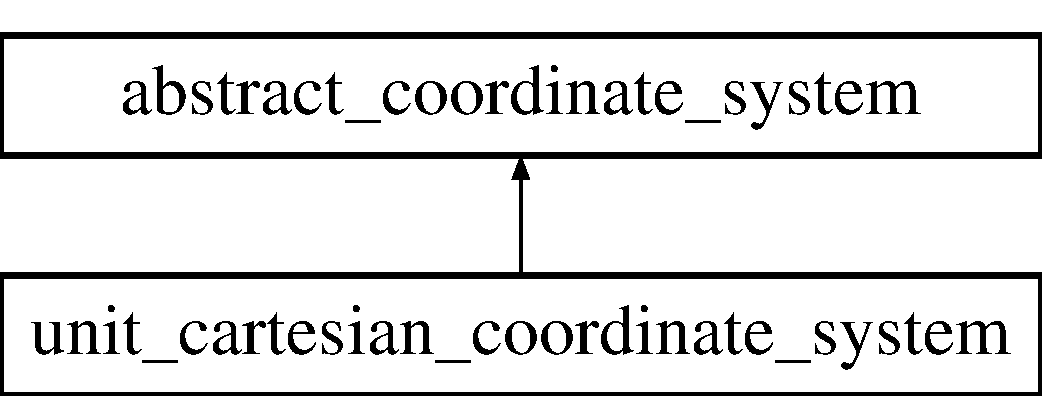
\includegraphics[height=2.000000cm]{classabstract__coordinate__system}
\end{center}
\end{figure}
\subsection*{Public Member Functions}
\begin{DoxyCompactItemize}
\item 
\hyperlink{classabstract__coordinate__system_ad6d5ae04c40f9c77a0aba70f4a7cb45e}{abstract\-\_\-coordinate\-\_\-system} ()
\item 
virtual void \hyperlink{classabstract__coordinate__system_a646c34b26579fa6f27ce00dcd8ab5951}{init} (sharedptr$<$ \hyperlink{classtile}{tile} $>$ t)=0
\item 
virtual float \hyperlink{classabstract__coordinate__system_a7df5507f5b2fddc0eb691e79514accab}{calc\-\_\-delta\-\_\-x} (long iw, long ih)=0
\item 
\hypertarget{classabstract__coordinate__system_a1129e984304df9036d3fcf548609ae08}{virtual float \hyperlink{classabstract__coordinate__system_a1129e984304df9036d3fcf548609ae08}{calc\-\_\-delta\-\_\-y} (long iw, long ih)=0}\label{classabstract__coordinate__system_a1129e984304df9036d3fcf548609ae08}

\begin{DoxyCompactList}\small\item\em See calc\-\_\-delta\-\_\-x\-\_\-at. \end{DoxyCompactList}\item 
\hypertarget{classabstract__coordinate__system_a09c21984f739869471dd2948b62b3191}{virtual float \hyperlink{classabstract__coordinate__system_a09c21984f739869471dd2948b62b3191}{calc\-\_\-x\-\_\-at} (long iw, long ih)=0}\label{classabstract__coordinate__system_a09c21984f739869471dd2948b62b3191}

\begin{DoxyCompactList}\small\item\em Calculate x coordinate at given pixel. \end{DoxyCompactList}\item 
\hypertarget{classabstract__coordinate__system_a2092dadc2aecf887bc8ca41d1fa65042}{virtual float \hyperlink{classabstract__coordinate__system_a2092dadc2aecf887bc8ca41d1fa65042}{calc\-\_\-y\-\_\-at} (long iw, long ih)=0}\label{classabstract__coordinate__system_a2092dadc2aecf887bc8ca41d1fa65042}

\begin{DoxyCompactList}\small\item\em Calculate y coordinate at given pixel. \end{DoxyCompactList}\end{DoxyCompactItemize}


\subsection{Detailed Description}
This is an abtstract class that calculates a coordinate (x,y) from an index (iw,ih) for a tile. Any derived class need not be cartesian but could also be polar.

U\-S\-A\-G\-E\-: Before the calc\-\_\-... methods can be called, the coordinate system has to be initialized with the given tile using the init(...) method. So the object itself just lays the rules for how to calculate a coordinate (x,y) from a given index (iw,ih). 

\subsection{Constructor \& Destructor Documentation}
\hypertarget{classabstract__coordinate__system_ad6d5ae04c40f9c77a0aba70f4a7cb45e}{\index{abstract\-\_\-coordinate\-\_\-system@{abstract\-\_\-coordinate\-\_\-system}!abstract\-\_\-coordinate\-\_\-system@{abstract\-\_\-coordinate\-\_\-system}}
\index{abstract\-\_\-coordinate\-\_\-system@{abstract\-\_\-coordinate\-\_\-system}!abstract_coordinate_system@{abstract\-\_\-coordinate\-\_\-system}}
\subsubsection[{abstract\-\_\-coordinate\-\_\-system}]{\setlength{\rightskip}{0pt plus 5cm}abstract\-\_\-coordinate\-\_\-system\-::abstract\-\_\-coordinate\-\_\-system (
\begin{DoxyParamCaption}
{}
\end{DoxyParamCaption}
)\hspace{0.3cm}{\ttfamily [inline]}}}\label{classabstract__coordinate__system_ad6d5ae04c40f9c77a0aba70f4a7cb45e}
Constructor. Before the coordinate system can be used, it has to be initialized with the given tile. Only after the init(...) method is called will the calculations functions give useful results. 

\subsection{Member Function Documentation}
\hypertarget{classabstract__coordinate__system_a7df5507f5b2fddc0eb691e79514accab}{\index{abstract\-\_\-coordinate\-\_\-system@{abstract\-\_\-coordinate\-\_\-system}!calc\-\_\-delta\-\_\-x@{calc\-\_\-delta\-\_\-x}}
\index{calc\-\_\-delta\-\_\-x@{calc\-\_\-delta\-\_\-x}!abstract_coordinate_system@{abstract\-\_\-coordinate\-\_\-system}}
\subsubsection[{calc\-\_\-delta\-\_\-x}]{\setlength{\rightskip}{0pt plus 5cm}virtual float abstract\-\_\-coordinate\-\_\-system\-::calc\-\_\-delta\-\_\-x (
\begin{DoxyParamCaption}
\item[{long}]{iw, }
\item[{long}]{ih}
\end{DoxyParamCaption}
)\hspace{0.3cm}{\ttfamily [pure virtual]}}}\label{classabstract__coordinate__system_a7df5507f5b2fddc0eb691e79514accab}
This is a method that returns the distance between neighboring points at point iw,ih. It was implemented to enable calculating the gradient in non equidistant coordinate systems (Jacobian). 
\begin{DoxyParams}{Parameters}
{\em iw} & \\
\hline
{\em ih} & \\
\hline
\end{DoxyParams}
\begin{DoxyReturn}{Returns}
deltax 
\end{DoxyReturn}


Implemented in \hyperlink{classunit__cartesian__coordinate__system_a9093a6700e1a34f6dfb127358973c8c5}{unit\-\_\-cartesian\-\_\-coordinate\-\_\-system}.

\hypertarget{classabstract__coordinate__system_a646c34b26579fa6f27ce00dcd8ab5951}{\index{abstract\-\_\-coordinate\-\_\-system@{abstract\-\_\-coordinate\-\_\-system}!init@{init}}
\index{init@{init}!abstract_coordinate_system@{abstract\-\_\-coordinate\-\_\-system}}
\subsubsection[{init}]{\setlength{\rightskip}{0pt plus 5cm}virtual void abstract\-\_\-coordinate\-\_\-system\-::init (
\begin{DoxyParamCaption}
\item[{sharedptr$<$ {\bf tile} $>$}]{t}
\end{DoxyParamCaption}
)\hspace{0.3cm}{\ttfamily [pure virtual]}}}\label{classabstract__coordinate__system_a646c34b26579fa6f27ce00dcd8ab5951}
This method initializes the coordinate system with the dimensions of the given tile. This method must be called before the calc\-\_\-... methods are called. 
\begin{DoxyParams}{Parameters}
{\em t} & \\
\hline
\end{DoxyParams}


Implemented in \hyperlink{classunit__cartesian__coordinate__system_a96d70a42cec4279c1320995e770c3fe5}{unit\-\_\-cartesian\-\_\-coordinate\-\_\-system}.



The documentation for this class was generated from the following file\-:\begin{DoxyCompactItemize}
\item 
include/tiles/abstract\-\_\-coordinate\-\_\-system.\-h\end{DoxyCompactItemize}

\hypertarget{classabstract__function}{\section{abstract\-\_\-function Class Reference}
\label{classabstract__function}\index{abstract\-\_\-function@{abstract\-\_\-function}}
}


{\ttfamily \#include $<$abstract\-\_\-function.\-h$>$}

Inheritance diagram for abstract\-\_\-function\-:\begin{figure}[H]
\begin{center}
\leavevmode
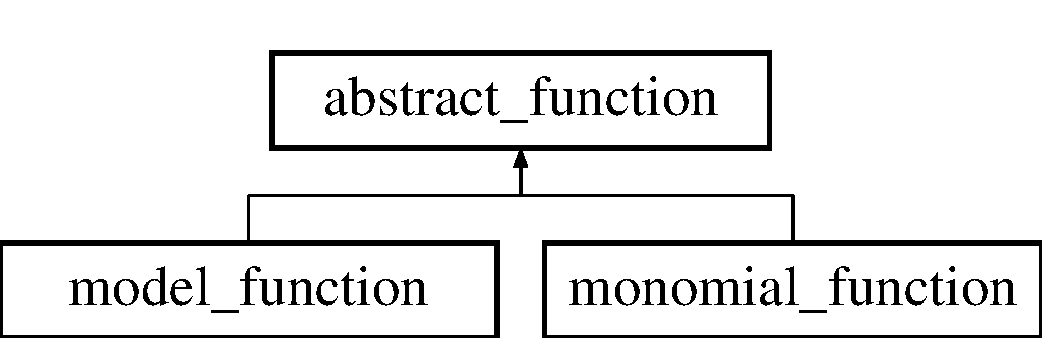
\includegraphics[height=2.000000cm]{classabstract__function}
\end{center}
\end{figure}
\subsection*{Public Member Functions}
\begin{DoxyCompactItemize}
\item 
virtual float \hyperlink{classabstract__function_ae313a63bae0ae1b88bcabd1bebc22f4f}{eval} (float x, float y)=0
\item 
virtual sharedptr\\*
$<$ \hyperlink{classabstract__gradient}{abstract\-\_\-gradient} $>$ \hyperlink{classabstract__function_a6ac83b83ed81cbd1c67ccfb9ddcf310b}{get\-\_\-gradient} ()=0
\end{DoxyCompactItemize}


\subsection{Detailed Description}
This pure virtual class provides an interface for the modeling functions f\-:R$^\wedge$2-\/$>$R 

\subsection{Member Function Documentation}
\hypertarget{classabstract__function_ae313a63bae0ae1b88bcabd1bebc22f4f}{\index{abstract\-\_\-function@{abstract\-\_\-function}!eval@{eval}}
\index{eval@{eval}!abstract_function@{abstract\-\_\-function}}
\subsubsection[{eval}]{\setlength{\rightskip}{0pt plus 5cm}virtual float abstract\-\_\-function\-::eval (
\begin{DoxyParamCaption}
\item[{float}]{x, }
\item[{float}]{y}
\end{DoxyParamCaption}
)\hspace{0.3cm}{\ttfamily [pure virtual]}}}\label{classabstract__function_ae313a63bae0ae1b88bcabd1bebc22f4f}
returns the value of the function at (x,y) 
\begin{DoxyParams}{Parameters}
{\em x} & coordinate \\
\hline
{\em y} & coordinate \\
\hline
\end{DoxyParams}
\begin{DoxyReturn}{Returns}
value of the function 
\end{DoxyReturn}


Implemented in \hyperlink{classmodel__function_a5ca38b00e9064eb46b697dab3b3e848f}{model\-\_\-function}, and \hyperlink{classmonomial__function_ac28af6c7f8c7c48216c7bdc270598728}{monomial\-\_\-function}.

\hypertarget{classabstract__function_a6ac83b83ed81cbd1c67ccfb9ddcf310b}{\index{abstract\-\_\-function@{abstract\-\_\-function}!get\-\_\-gradient@{get\-\_\-gradient}}
\index{get\-\_\-gradient@{get\-\_\-gradient}!abstract_function@{abstract\-\_\-function}}
\subsubsection[{get\-\_\-gradient}]{\setlength{\rightskip}{0pt plus 5cm}virtual sharedptr$<${\bf abstract\-\_\-gradient}$>$ abstract\-\_\-function\-::get\-\_\-gradient (
\begin{DoxyParamCaption}
{}
\end{DoxyParamCaption}
)\hspace{0.3cm}{\ttfamily [pure virtual]}}}\label{classabstract__function_a6ac83b83ed81cbd1c67ccfb9ddcf310b}
Get the gradient function of this base function \begin{DoxyReturn}{Returns}
gradient function 
\end{DoxyReturn}


Implemented in \hyperlink{classmodel__function_adf3a7a6ff204c7e993f63f61cd2cfcf1}{model\-\_\-function}, and \hyperlink{classmonomial__function_a1bb8949943f068e0597c7a8983011d12}{monomial\-\_\-function}.



The documentation for this class was generated from the following file\-:\begin{DoxyCompactItemize}
\item 
include/model/abstract\-\_\-function.\-h\end{DoxyCompactItemize}

\hypertarget{classabstract__gradient}{\section{abstract\-\_\-gradient Class Reference}
\label{classabstract__gradient}\index{abstract\-\_\-gradient@{abstract\-\_\-gradient}}
}
Inheritance diagram for abstract\-\_\-gradient\-:\begin{figure}[H]
\begin{center}
\leavevmode
\includegraphics[height=2.000000cm]{classabstract__gradient}
\end{center}
\end{figure}
\subsection*{Public Member Functions}
\begin{DoxyCompactItemize}
\item 
virtual sharedarray$<$ float $>$ \hyperlink{classabstract__gradient_a4720548702baebd45572547fd913ef30}{eval} (float x, float y)=0
\end{DoxyCompactItemize}


\subsection{Member Function Documentation}
\hypertarget{classabstract__gradient_a4720548702baebd45572547fd913ef30}{\index{abstract\-\_\-gradient@{abstract\-\_\-gradient}!eval@{eval}}
\index{eval@{eval}!abstract_gradient@{abstract\-\_\-gradient}}
\subsubsection[{eval}]{\setlength{\rightskip}{0pt plus 5cm}virtual sharedarray$<$float$>$ abstract\-\_\-gradient\-::eval (
\begin{DoxyParamCaption}
\item[{float}]{x, }
\item[{float}]{y}
\end{DoxyParamCaption}
)\hspace{0.3cm}{\ttfamily [pure virtual]}}}\label{classabstract__gradient_a4720548702baebd45572547fd913ef30}
returns the value of the function at (x,y) 
\begin{DoxyParams}{Parameters}
{\em x} & coordinate \\
\hline
{\em y} & coordinate \\
\hline
\end{DoxyParams}
\begin{DoxyReturn}{Returns}
value of the gradient function in x and y 
\end{DoxyReturn}


Implemented in \hyperlink{classmonomial__gradient_a718fe4bdf3a6edd32d655de03db8badf}{monomial\-\_\-gradient}, and \hyperlink{classmodel__gradient_a3342773b28b53352dfd08abd25b946f6}{model\-\_\-gradient}.



The documentation for this class was generated from the following file\-:\begin{DoxyCompactItemize}
\item 
include/model/abstract\-\_\-gradient.\-h\end{DoxyCompactItemize}

\hypertarget{classabstract__gradient__calculator}{\section{abstract\-\_\-gradient\-\_\-calculator Class Reference}
\label{classabstract__gradient__calculator}\index{abstract\-\_\-gradient\-\_\-calculator@{abstract\-\_\-gradient\-\_\-calculator}}
}
Inheritance diagram for abstract\-\_\-gradient\-\_\-calculator\-:\begin{figure}[H]
\begin{center}
\leavevmode
\includegraphics[height=2.000000cm]{classabstract__gradient__calculator}
\end{center}
\end{figure}
\subsection*{Public Member Functions}
\begin{DoxyCompactItemize}
\item 
\hyperlink{classabstract__gradient__calculator_a259548d80ec064ee93f8342bbd9d16f3}{abstract\-\_\-gradient\-\_\-calculator} ()
\item 
\hypertarget{classabstract__gradient__calculator_ad492fd85c34849194dc566f32d93e641}{virtual \hyperlink{classabstract__gradient__calculator_ad492fd85c34849194dc566f32d93e641}{$\sim$abstract\-\_\-gradient\-\_\-calculator} ()}\label{classabstract__gradient__calculator_ad492fd85c34849194dc566f32d93e641}

\begin{DoxyCompactList}\small\item\em Destructor. \end{DoxyCompactList}\item 
virtual sharedptr$<$ std\-::vector\\*
$<$ \hyperlink{classtile}{tile} $>$ $>$ \hyperlink{classabstract__gradient__calculator_a18d3f5191a95f8a3bfeb7b79862c0f24}{get\-\_\-gradient\-\_\-tile} (sharedptr$<$ \hyperlink{classtile}{tile} $>$ t)
\item 
virtual sharedptr$<$ std\-::vector\\*
$<$ float $>$ $>$ \hyperlink{classabstract__gradient__calculator_afbc6ee285d21d21b2241cfe643f8adce}{get\-\_\-gradient\-\_\-floats} (sharedptr$<$ \hyperlink{classtile}{tile} $>$ t)=0
\item 
virtual sharedptr\\*
$<$ Eigen\-::\-Vector\-Xf $>$ \hyperlink{classabstract__gradient__calculator_ae101a124df59f5dbcc4d21acffe43ae1}{get\-\_\-gradient\-\_\-eigen\-\_\-vector} (sharedptr$<$ \hyperlink{classtile}{tile} $>$ t)=0
\end{DoxyCompactItemize}


\subsection{Constructor \& Destructor Documentation}
\hypertarget{classabstract__gradient__calculator_a259548d80ec064ee93f8342bbd9d16f3}{\index{abstract\-\_\-gradient\-\_\-calculator@{abstract\-\_\-gradient\-\_\-calculator}!abstract\-\_\-gradient\-\_\-calculator@{abstract\-\_\-gradient\-\_\-calculator}}
\index{abstract\-\_\-gradient\-\_\-calculator@{abstract\-\_\-gradient\-\_\-calculator}!abstract_gradient_calculator@{abstract\-\_\-gradient\-\_\-calculator}}
\subsubsection[{abstract\-\_\-gradient\-\_\-calculator}]{\setlength{\rightskip}{0pt plus 5cm}abstract\-\_\-gradient\-\_\-calculator\-::abstract\-\_\-gradient\-\_\-calculator (
\begin{DoxyParamCaption}
{}
\end{DoxyParamCaption}
)\hspace{0.3cm}{\ttfamily [inline]}}}\label{classabstract__gradient__calculator_a259548d80ec064ee93f8342bbd9d16f3}
This constructor takes a pointer to an abstract\-\_\-coordinate system. This coordinate system is then used to calculate the derivative for the given tile in the get\-\_\-gradient\-\_\-... methods. 
\begin{DoxyParams}{Parameters}
{\em coord\-\_\-sys} & \\
\hline
\end{DoxyParams}


\subsection{Member Function Documentation}
\hypertarget{classabstract__gradient__calculator_ae101a124df59f5dbcc4d21acffe43ae1}{\index{abstract\-\_\-gradient\-\_\-calculator@{abstract\-\_\-gradient\-\_\-calculator}!get\-\_\-gradient\-\_\-eigen\-\_\-vector@{get\-\_\-gradient\-\_\-eigen\-\_\-vector}}
\index{get\-\_\-gradient\-\_\-eigen\-\_\-vector@{get\-\_\-gradient\-\_\-eigen\-\_\-vector}!abstract_gradient_calculator@{abstract\-\_\-gradient\-\_\-calculator}}
\subsubsection[{get\-\_\-gradient\-\_\-eigen\-\_\-vector}]{\setlength{\rightskip}{0pt plus 5cm}virtual sharedptr$<$Eigen\-::\-Vector\-Xf$>$ abstract\-\_\-gradient\-\_\-calculator\-::get\-\_\-gradient\-\_\-eigen\-\_\-vector (
\begin{DoxyParamCaption}
\item[{sharedptr$<$ {\bf tile} $>$}]{t}
\end{DoxyParamCaption}
)\hspace{0.3cm}{\ttfamily [pure virtual]}}}\label{classabstract__gradient__calculator_ae101a124df59f5dbcc4d21acffe43ae1}
Get the gradient of a given tile as a Eigen\-::\-Vector of floats 
\begin{DoxyParams}{Parameters}
{\em t} & tile \\
\hline
\end{DoxyParams}
\begin{DoxyReturn}{Returns}
Eigen\-::vector of floats, first holds the x-\/gradient-\/values in order of tile has in its vector. Second holds y... 
\end{DoxyReturn}


Implemented in \hyperlink{classsecond__order__gradient_a920ecf0cbc89fa73782a318186cc3a6b}{second\-\_\-order\-\_\-gradient}.

\hypertarget{classabstract__gradient__calculator_afbc6ee285d21d21b2241cfe643f8adce}{\index{abstract\-\_\-gradient\-\_\-calculator@{abstract\-\_\-gradient\-\_\-calculator}!get\-\_\-gradient\-\_\-floats@{get\-\_\-gradient\-\_\-floats}}
\index{get\-\_\-gradient\-\_\-floats@{get\-\_\-gradient\-\_\-floats}!abstract_gradient_calculator@{abstract\-\_\-gradient\-\_\-calculator}}
\subsubsection[{get\-\_\-gradient\-\_\-floats}]{\setlength{\rightskip}{0pt plus 5cm}virtual sharedptr$<$std\-::vector$<$float$>$ $>$ abstract\-\_\-gradient\-\_\-calculator\-::get\-\_\-gradient\-\_\-floats (
\begin{DoxyParamCaption}
\item[{sharedptr$<$ {\bf tile} $>$}]{t}
\end{DoxyParamCaption}
)\hspace{0.3cm}{\ttfamily [pure virtual]}}}\label{classabstract__gradient__calculator_afbc6ee285d21d21b2241cfe643f8adce}
Get the gradient of a given tile as raw float data. 
\begin{DoxyParams}{Parameters}
{\em t} & tile \\
\hline
\end{DoxyParams}
\begin{DoxyReturn}{Returns}
vector of floats, first holding the x-\/gradient-\/values in same order which the data array of the tiles stores the values. Afterwards appending the y-\/values... 
\end{DoxyReturn}


Implemented in \hyperlink{classsecond__order__gradient_a611bd811d9a47b0a53b7a827344189ff}{second\-\_\-order\-\_\-gradient}.

\hypertarget{classabstract__gradient__calculator_a18d3f5191a95f8a3bfeb7b79862c0f24}{\index{abstract\-\_\-gradient\-\_\-calculator@{abstract\-\_\-gradient\-\_\-calculator}!get\-\_\-gradient\-\_\-tile@{get\-\_\-gradient\-\_\-tile}}
\index{get\-\_\-gradient\-\_\-tile@{get\-\_\-gradient\-\_\-tile}!abstract_gradient_calculator@{abstract\-\_\-gradient\-\_\-calculator}}
\subsubsection[{get\-\_\-gradient\-\_\-tile}]{\setlength{\rightskip}{0pt plus 5cm}sharedptr$<$ std\-::vector$<$ {\bf tile} $>$ $>$ abstract\-\_\-gradient\-\_\-calculator\-::get\-\_\-gradient\-\_\-tile (
\begin{DoxyParamCaption}
\item[{sharedptr$<$ {\bf tile} $>$}]{t}
\end{DoxyParamCaption}
)\hspace{0.3cm}{\ttfamily [virtual]}}}\label{classabstract__gradient__calculator_a18d3f5191a95f8a3bfeb7b79862c0f24}
Get the gradient of a given tile in the tile-\/format. First element of the vector will be a tile representing the x gradient and second element will be a tile representing the y gradient. This method is for debug purposes mostly since it will call the abstract get\-\_\-gradient\-\_\-floats method of the instance. 
\begin{DoxyParams}{Parameters}
{\em t} & tile \\
\hline
\end{DoxyParams}
\begin{DoxyReturn}{Returns}
gradient of given tile in x and y direction. x is first, y is second 
\end{DoxyReturn}


The documentation for this class was generated from the following files\-:\begin{DoxyCompactItemize}
\item 
include/algorithm/abstract\-\_\-gradient\-\_\-calculator.\-h\item 
src/algorithm/abstract\-\_\-gradient\-\_\-calculator.\-cpp\end{DoxyCompactItemize}

\hypertarget{classabstract__reliability__calculator}{\section{abstract\-\_\-reliability\-\_\-calculator Class Reference}
\label{classabstract__reliability__calculator}\index{abstract\-\_\-reliability\-\_\-calculator@{abstract\-\_\-reliability\-\_\-calculator}}
}


{\ttfamily \#include $<$abstract\-\_\-reliability\-\_\-calculator.\-h$>$}

Inheritance diagram for abstract\-\_\-reliability\-\_\-calculator\-:\begin{figure}[H]
\begin{center}
\leavevmode
\includegraphics[height=1.171548cm]{classabstract__reliability__calculator}
\end{center}
\end{figure}
\subsection*{Public Member Functions}
\begin{DoxyCompactItemize}
\item 
\hyperlink{classabstract__reliability__calculator_ac28dfe44888c3beb9d6ceeaeea1c99a7}{abstract\-\_\-reliability\-\_\-calculator} ()
\item 
virtual float \hyperlink{classabstract__reliability__calculator_a0c9a7778550b643b6a273e3bf0662023}{calculate\-\_\-reliability} (boost\-::shared\-\_\-ptr$<$ \hyperlink{classtiled__image}{tiled\-\_\-image} $>$ ti, boost\-::shared\-\_\-ptr$<$ \hyperlink{classtile__junction}{tile\-\_\-junction} $>$ junc)=0
\item 
virtual float \hyperlink{classabstract__reliability__calculator_a496b1743c17660ae4617eebdd312bb9d}{calculate\-\_\-reliability} (boost\-::shared\-\_\-ptr$<$ \hyperlink{classtiled__image}{tiled\-\_\-image} $>$ ti, boost\-::shared\-\_\-ptr$<$ \hyperlink{classtile}{tile} $>$ t)=0
\item 
virtual void \hyperlink{classabstract__reliability__calculator_a4457d3eece3c873e2cc2455a6dfdbb88}{init\-\_\-junctions} (sharedptr$<$ \hyperlink{classtiled__image}{tiled\-\_\-image} $>$ ti)=0
\end{DoxyCompactItemize}


\subsection{Detailed Description}
This pure virtual class provides an abstract interface for a reliability calculating class. Such a class must implement a function for calculating the reliability of a given junction and of a given tile. 

\subsection{Constructor \& Destructor Documentation}
\hypertarget{classabstract__reliability__calculator_ac28dfe44888c3beb9d6ceeaeea1c99a7}{\index{abstract\-\_\-reliability\-\_\-calculator@{abstract\-\_\-reliability\-\_\-calculator}!abstract\-\_\-reliability\-\_\-calculator@{abstract\-\_\-reliability\-\_\-calculator}}
\index{abstract\-\_\-reliability\-\_\-calculator@{abstract\-\_\-reliability\-\_\-calculator}!abstract_reliability_calculator@{abstract\-\_\-reliability\-\_\-calculator}}
\subsubsection[{abstract\-\_\-reliability\-\_\-calculator}]{\setlength{\rightskip}{0pt plus 5cm}abstract\-\_\-reliability\-\_\-calculator\-::abstract\-\_\-reliability\-\_\-calculator (
\begin{DoxyParamCaption}
{}
\end{DoxyParamCaption}
)\hspace{0.3cm}{\ttfamily [inline]}}}\label{classabstract__reliability__calculator_ac28dfe44888c3beb9d6ceeaeea1c99a7}
Constructor 

\subsection{Member Function Documentation}
\hypertarget{classabstract__reliability__calculator_a0c9a7778550b643b6a273e3bf0662023}{\index{abstract\-\_\-reliability\-\_\-calculator@{abstract\-\_\-reliability\-\_\-calculator}!calculate\-\_\-reliability@{calculate\-\_\-reliability}}
\index{calculate\-\_\-reliability@{calculate\-\_\-reliability}!abstract_reliability_calculator@{abstract\-\_\-reliability\-\_\-calculator}}
\subsubsection[{calculate\-\_\-reliability}]{\setlength{\rightskip}{0pt plus 5cm}virtual float abstract\-\_\-reliability\-\_\-calculator\-::calculate\-\_\-reliability (
\begin{DoxyParamCaption}
\item[{boost\-::shared\-\_\-ptr$<$ {\bf tiled\-\_\-image} $>$}]{ti, }
\item[{boost\-::shared\-\_\-ptr$<$ {\bf tile\-\_\-junction} $>$}]{junc}
\end{DoxyParamCaption}
)\hspace{0.3cm}{\ttfamily [pure virtual]}}}\label{classabstract__reliability__calculator_a0c9a7778550b643b6a273e3bf0662023}
Calculates the reliability of a given junction 
\begin{DoxyParams}{Parameters}
{\em ti} & tiled image \\
\hline
{\em junc} & junction \\
\hline
\end{DoxyParams}


Implemented in \hyperlink{classreliability__calculator__random_a73524f3dd704cb666c794b765e4216fc}{reliability\-\_\-calculator\-\_\-random}, \hyperlink{classreliability__calculator__variance__second_a1150171c57a7b9420e5f5211e71c265a}{reliability\-\_\-calculator\-\_\-variance\-\_\-second}, \hyperlink{classreliability__calculator__variance_ac6380a3bedfdc5648f501cd0a5c92369}{reliability\-\_\-calculator\-\_\-variance}, and \hyperlink{classreliability__calculator__mean__difference_a2d64711ed370d44aae8c276e1507ee4a}{reliability\-\_\-calculator\-\_\-mean\-\_\-difference}.

\hypertarget{classabstract__reliability__calculator_a496b1743c17660ae4617eebdd312bb9d}{\index{abstract\-\_\-reliability\-\_\-calculator@{abstract\-\_\-reliability\-\_\-calculator}!calculate\-\_\-reliability@{calculate\-\_\-reliability}}
\index{calculate\-\_\-reliability@{calculate\-\_\-reliability}!abstract_reliability_calculator@{abstract\-\_\-reliability\-\_\-calculator}}
\subsubsection[{calculate\-\_\-reliability}]{\setlength{\rightskip}{0pt plus 5cm}virtual float abstract\-\_\-reliability\-\_\-calculator\-::calculate\-\_\-reliability (
\begin{DoxyParamCaption}
\item[{boost\-::shared\-\_\-ptr$<$ {\bf tiled\-\_\-image} $>$}]{ti, }
\item[{boost\-::shared\-\_\-ptr$<$ {\bf tile} $>$}]{t}
\end{DoxyParamCaption}
)\hspace{0.3cm}{\ttfamily [pure virtual]}}}\label{classabstract__reliability__calculator_a496b1743c17660ae4617eebdd312bb9d}
Calculates the reliability of a given tile 
\begin{DoxyParams}{Parameters}
{\em ti} & tiled image \\
\hline
{\em t} & tile \\
\hline
\end{DoxyParams}


Implemented in \hyperlink{classreliability__calculator__variance__second_a0cab62b334c6f20aa821496f7364bd98}{reliability\-\_\-calculator\-\_\-variance\-\_\-second}, \hyperlink{classreliability__calculator__random_a7e49000129535b04968a5fb7a87fd5e4}{reliability\-\_\-calculator\-\_\-random}, \hyperlink{classreliability__calculator__variance_a0250bc0b9f2d62ec48b66449d6f94b56}{reliability\-\_\-calculator\-\_\-variance}, and \hyperlink{classreliability__calculator__mean__difference_a9e03f2bdf2a04d9a414530598db0cbf4}{reliability\-\_\-calculator\-\_\-mean\-\_\-difference}.

\hypertarget{classabstract__reliability__calculator_a4457d3eece3c873e2cc2455a6dfdbb88}{\index{abstract\-\_\-reliability\-\_\-calculator@{abstract\-\_\-reliability\-\_\-calculator}!init\-\_\-junctions@{init\-\_\-junctions}}
\index{init\-\_\-junctions@{init\-\_\-junctions}!abstract_reliability_calculator@{abstract\-\_\-reliability\-\_\-calculator}}
\subsubsection[{init\-\_\-junctions}]{\setlength{\rightskip}{0pt plus 5cm}virtual void abstract\-\_\-reliability\-\_\-calculator\-::init\-\_\-junctions (
\begin{DoxyParamCaption}
\item[{sharedptr$<$ {\bf tiled\-\_\-image} $>$}]{ti}
\end{DoxyParamCaption}
)\hspace{0.3cm}{\ttfamily [pure virtual]}}}\label{classabstract__reliability__calculator_a4457d3eece3c873e2cc2455a6dfdbb88}
Calculate the variance of each junction once, therefor making it possible to just access them via get\-\_\-variance. 
\begin{DoxyParams}{Parameters}
{\em ti} & tiled image \\
\hline
\end{DoxyParams}


Implemented in \hyperlink{classreliability__calculator__random_a3b5b45c3e398b70398ba139eb6046dc5}{reliability\-\_\-calculator\-\_\-random}, \hyperlink{classreliability__calculator__variance_ad371792568036db7a8dac6fabbb78d05}{reliability\-\_\-calculator\-\_\-variance}, \hyperlink{classreliability__calculator__variance__second_a5c7dcb23c303a0ec762504ea9a775b2b}{reliability\-\_\-calculator\-\_\-variance\-\_\-second}, and \hyperlink{classreliability__calculator__mean__difference_a6a49bd9cf9996cdee5919f2307ca473a}{reliability\-\_\-calculator\-\_\-mean\-\_\-difference}.



The documentation for this class was generated from the following file\-:\begin{DoxyCompactItemize}
\item 
include/algorithm/abstract\-\_\-reliability\-\_\-calculator.\-h\end{DoxyCompactItemize}

\hypertarget{classabstract__tile__merger}{\section{abstract\-\_\-tile\-\_\-merger Class Reference}
\label{classabstract__tile__merger}\index{abstract\-\_\-tile\-\_\-merger@{abstract\-\_\-tile\-\_\-merger}}
}


{\ttfamily \#include $<$abstract\-\_\-tile\-\_\-merger.\-h$>$}

Inheritance diagram for abstract\-\_\-tile\-\_\-merger\-:\begin{figure}[H]
\begin{center}
\leavevmode
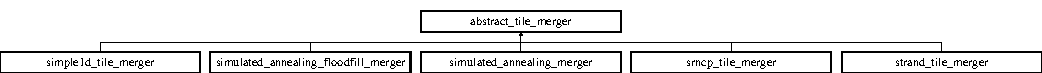
\includegraphics[height=0.978166cm]{classabstract__tile__merger}
\end{center}
\end{figure}
\subsection*{Public Member Functions}
\begin{DoxyCompactItemize}
\item 
\hyperlink{classabstract__tile__merger_a69c603d54ddfaf3346713756bfceaab5}{abstract\-\_\-tile\-\_\-merger} ()
\item 
virtual void \hyperlink{classabstract__tile__merger_a52ab494f77e495ab1a59b49e49c98db4}{merge\-\_\-tiles} (boost\-::shared\-\_\-ptr$<$ \hyperlink{classtiled__image}{tiled\-\_\-image} $>$ t)=0
\item 
virtual std\-::string \hyperlink{classabstract__tile__merger_a12ec9d118912b3c571d61ff9649042c6}{get\-\_\-name} ()=0
\item 
virtual void \hyperlink{classabstract__tile__merger_a7922b65624d12ef2d6c115218d2378b4}{usage\-\_\-help} ()=0
\end{DoxyCompactItemize}


\subsection{Detailed Description}
This pure virtual class provides an abstract interface for an merger that merges all tiles of a smart tiled image. It operates with boost smart pointers. 

\subsection{Constructor \& Destructor Documentation}
\hypertarget{classabstract__tile__merger_a69c603d54ddfaf3346713756bfceaab5}{\index{abstract\-\_\-tile\-\_\-merger@{abstract\-\_\-tile\-\_\-merger}!abstract\-\_\-tile\-\_\-merger@{abstract\-\_\-tile\-\_\-merger}}
\index{abstract\-\_\-tile\-\_\-merger@{abstract\-\_\-tile\-\_\-merger}!abstract_tile_merger@{abstract\-\_\-tile\-\_\-merger}}
\subsubsection[{abstract\-\_\-tile\-\_\-merger}]{\setlength{\rightskip}{0pt plus 5cm}abstract\-\_\-tile\-\_\-merger\-::abstract\-\_\-tile\-\_\-merger (
\begin{DoxyParamCaption}
{}
\end{DoxyParamCaption}
)\hspace{0.3cm}{\ttfamily [inline]}}}\label{classabstract__tile__merger_a69c603d54ddfaf3346713756bfceaab5}
Konstruktor 

\subsection{Member Function Documentation}
\hypertarget{classabstract__tile__merger_a12ec9d118912b3c571d61ff9649042c6}{\index{abstract\-\_\-tile\-\_\-merger@{abstract\-\_\-tile\-\_\-merger}!get\-\_\-name@{get\-\_\-name}}
\index{get\-\_\-name@{get\-\_\-name}!abstract_tile_merger@{abstract\-\_\-tile\-\_\-merger}}
\subsubsection[{get\-\_\-name}]{\setlength{\rightskip}{0pt plus 5cm}virtual std\-::string abstract\-\_\-tile\-\_\-merger\-::get\-\_\-name (
\begin{DoxyParamCaption}
{}
\end{DoxyParamCaption}
)\hspace{0.3cm}{\ttfamily [pure virtual]}}}\label{classabstract__tile__merger_a12ec9d118912b3c571d61ff9649042c6}
Return a name (with options) to set in the output file name 

Implemented in \hyperlink{classsimulated__annealing__floodfill__merger_a1e235b700efd2ccdcf771cd93251a1b9}{simulated\-\_\-annealing\-\_\-floodfill\-\_\-merger}, \hyperlink{classsimulated__annealing__merger_a2548233017acafb226be7bcdb2c91e22}{simulated\-\_\-annealing\-\_\-merger}, \hyperlink{classsrncp__tile__merger_a7e6fb5b07129a1354a8d997161b210c4}{srncp\-\_\-tile\-\_\-merger}, \hyperlink{classsimple1d__tile__merger_ac0810b20cdeb08613cb2a214267cf26a}{simple1d\-\_\-tile\-\_\-merger}, and \hyperlink{classstrand__tile__merger_a3e548d789df5b5a39435c095dd51365b}{strand\-\_\-tile\-\_\-merger}.

\hypertarget{classabstract__tile__merger_a52ab494f77e495ab1a59b49e49c98db4}{\index{abstract\-\_\-tile\-\_\-merger@{abstract\-\_\-tile\-\_\-merger}!merge\-\_\-tiles@{merge\-\_\-tiles}}
\index{merge\-\_\-tiles@{merge\-\_\-tiles}!abstract_tile_merger@{abstract\-\_\-tile\-\_\-merger}}
\subsubsection[{merge\-\_\-tiles}]{\setlength{\rightskip}{0pt plus 5cm}virtual void abstract\-\_\-tile\-\_\-merger\-::merge\-\_\-tiles (
\begin{DoxyParamCaption}
\item[{boost\-::shared\-\_\-ptr$<$ {\bf tiled\-\_\-image} $>$}]{t}
\end{DoxyParamCaption}
)\hspace{0.3cm}{\ttfamily [pure virtual]}}}\label{classabstract__tile__merger_a52ab494f77e495ab1a59b49e49c98db4}
Merge all given tiles inside the smart tiled image 
\begin{DoxyParams}{Parameters}
{\em t} & boost shared\-\_\-ptr to smart tiled image \\
\hline
\end{DoxyParams}


Implemented in \hyperlink{classsrncp__tile__merger_ad8330c73633437c5f4860d837bf63345}{srncp\-\_\-tile\-\_\-merger}, and \hyperlink{classsimple1d__tile__merger_ad73f710dd3ea0116859dcf2e5f6c5a14}{simple1d\-\_\-tile\-\_\-merger}.

\hypertarget{classabstract__tile__merger_a7922b65624d12ef2d6c115218d2378b4}{\index{abstract\-\_\-tile\-\_\-merger@{abstract\-\_\-tile\-\_\-merger}!usage\-\_\-help@{usage\-\_\-help}}
\index{usage\-\_\-help@{usage\-\_\-help}!abstract_tile_merger@{abstract\-\_\-tile\-\_\-merger}}
\subsubsection[{usage\-\_\-help}]{\setlength{\rightskip}{0pt plus 5cm}virtual void abstract\-\_\-tile\-\_\-merger\-::usage\-\_\-help (
\begin{DoxyParamCaption}
{}
\end{DoxyParamCaption}
)\hspace{0.3cm}{\ttfamily [pure virtual]}}}\label{classabstract__tile__merger_a7922b65624d12ef2d6c115218d2378b4}
Display a help on how to use this merger, in particular usage of merger-\/settings 

Implemented in \hyperlink{classsimulated__annealing__floodfill__merger_a6470774a227b289d5e16beac41e163d2}{simulated\-\_\-annealing\-\_\-floodfill\-\_\-merger}, \hyperlink{classsimulated__annealing__merger_a34ac2a006a40fe0b4e57c6868803bf07}{simulated\-\_\-annealing\-\_\-merger}, \hyperlink{classsrncp__tile__merger_ae57137ab8a1df19b86c28d3ff4aa1d9e}{srncp\-\_\-tile\-\_\-merger}, \hyperlink{classsimple1d__tile__merger_a4f18628ddf20f24efc13e705b469268c}{simple1d\-\_\-tile\-\_\-merger}, and \hyperlink{classstrand__tile__merger_af623214f3fe92b402d1a5510f1208071}{strand\-\_\-tile\-\_\-merger}.



The documentation for this class was generated from the following file\-:\begin{DoxyCompactItemize}
\item 
include/algorithm/abstract\-\_\-tile\-\_\-merger.\-h\end{DoxyCompactItemize}

\hypertarget{classabstract__tile__unwrapper}{\section{abstract\-\_\-tile\-\_\-unwrapper Class Reference}
\label{classabstract__tile__unwrapper}\index{abstract\-\_\-tile\-\_\-unwrapper@{abstract\-\_\-tile\-\_\-unwrapper}}
}


{\ttfamily \#include $<$abstract\-\_\-tile\-\_\-unwrapper.\-h$>$}

Inheritance diagram for abstract\-\_\-tile\-\_\-unwrapper\-:\begin{figure}[H]
\begin{center}
\leavevmode
\includegraphics[height=1.885522cm]{classabstract__tile__unwrapper}
\end{center}
\end{figure}
\subsection*{Public Member Functions}
\begin{DoxyCompactItemize}
\item 
\hyperlink{classabstract__tile__unwrapper_a31fc3a41d4adaab0ba7c2998e74ccedb}{abstract\-\_\-tile\-\_\-unwrapper} ()
\item 
virtual void \hyperlink{classabstract__tile__unwrapper_a74eedd36e55b9000b5986ff5980a563a}{unwrap} (boost\-::shared\-\_\-ptr$<$ \hyperlink{classtile}{tile} $>$ t)=0
\item 
virtual std\-::string \hyperlink{classabstract__tile__unwrapper_ae70f69a703e622e5ab13eabcc91fca4d}{get\-\_\-name} ()=0
\item 
virtual void \hyperlink{classabstract__tile__unwrapper_a469b36a7f302d5a2655631bbdb6f8daf}{usage\-\_\-help} ()=0
\end{DoxyCompactItemize}


\subsection{Detailed Description}
This pure virtual class provides an abstract interface for an unwrapper that unwraps a single tile. It operates with boost smart pointers. 

\subsection{Constructor \& Destructor Documentation}
\hypertarget{classabstract__tile__unwrapper_a31fc3a41d4adaab0ba7c2998e74ccedb}{\index{abstract\-\_\-tile\-\_\-unwrapper@{abstract\-\_\-tile\-\_\-unwrapper}!abstract\-\_\-tile\-\_\-unwrapper@{abstract\-\_\-tile\-\_\-unwrapper}}
\index{abstract\-\_\-tile\-\_\-unwrapper@{abstract\-\_\-tile\-\_\-unwrapper}!abstract_tile_unwrapper@{abstract\-\_\-tile\-\_\-unwrapper}}
\subsubsection[{abstract\-\_\-tile\-\_\-unwrapper}]{\setlength{\rightskip}{0pt plus 5cm}abstract\-\_\-tile\-\_\-unwrapper\-::abstract\-\_\-tile\-\_\-unwrapper (
\begin{DoxyParamCaption}
{}
\end{DoxyParamCaption}
)\hspace{0.3cm}{\ttfamily [inline]}}}\label{classabstract__tile__unwrapper_a31fc3a41d4adaab0ba7c2998e74ccedb}
Konstruktor 

\subsection{Member Function Documentation}
\hypertarget{classabstract__tile__unwrapper_ae70f69a703e622e5ab13eabcc91fca4d}{\index{abstract\-\_\-tile\-\_\-unwrapper@{abstract\-\_\-tile\-\_\-unwrapper}!get\-\_\-name@{get\-\_\-name}}
\index{get\-\_\-name@{get\-\_\-name}!abstract_tile_unwrapper@{abstract\-\_\-tile\-\_\-unwrapper}}
\subsubsection[{get\-\_\-name}]{\setlength{\rightskip}{0pt plus 5cm}virtual std\-::string abstract\-\_\-tile\-\_\-unwrapper\-::get\-\_\-name (
\begin{DoxyParamCaption}
{}
\end{DoxyParamCaption}
)\hspace{0.3cm}{\ttfamily [pure virtual]}}}\label{classabstract__tile__unwrapper_ae70f69a703e622e5ab13eabcc91fca4d}
Return a name (with options) to set in the output file name 

Implemented in \hyperlink{classleast__squares__grad__unwrapper_af66d1a659d6cfbb82200d120f43dd939}{least\-\_\-squares\-\_\-grad\-\_\-unwrapper}, \hyperlink{classstrand__tile__unwrapper_ae4ce9d7459840ada66b7492ea2873969}{strand\-\_\-tile\-\_\-unwrapper}, and \hyperlink{classgrad__fit__tile__unwrapper_a46a71a2adc53411289f792aae8c1b61c}{grad\-\_\-fit\-\_\-tile\-\_\-unwrapper}.

\hypertarget{classabstract__tile__unwrapper_a74eedd36e55b9000b5986ff5980a563a}{\index{abstract\-\_\-tile\-\_\-unwrapper@{abstract\-\_\-tile\-\_\-unwrapper}!unwrap@{unwrap}}
\index{unwrap@{unwrap}!abstract_tile_unwrapper@{abstract\-\_\-tile\-\_\-unwrapper}}
\subsubsection[{unwrap}]{\setlength{\rightskip}{0pt plus 5cm}virtual void abstract\-\_\-tile\-\_\-unwrapper\-::unwrap (
\begin{DoxyParamCaption}
\item[{boost\-::shared\-\_\-ptr$<$ {\bf tile} $>$}]{t}
\end{DoxyParamCaption}
)\hspace{0.3cm}{\ttfamily [pure virtual]}}}\label{classabstract__tile__unwrapper_a74eedd36e55b9000b5986ff5980a563a}
Unwrap a given tile. 
\begin{DoxyParams}{Parameters}
{\em t} & \\
\hline
\end{DoxyParams}


Implemented in \hyperlink{classstrand__tile__unwrapper_a520d7832e80746c9996fe042b5993235}{strand\-\_\-tile\-\_\-unwrapper}.

\hypertarget{classabstract__tile__unwrapper_a469b36a7f302d5a2655631bbdb6f8daf}{\index{abstract\-\_\-tile\-\_\-unwrapper@{abstract\-\_\-tile\-\_\-unwrapper}!usage\-\_\-help@{usage\-\_\-help}}
\index{usage\-\_\-help@{usage\-\_\-help}!abstract_tile_unwrapper@{abstract\-\_\-tile\-\_\-unwrapper}}
\subsubsection[{usage\-\_\-help}]{\setlength{\rightskip}{0pt plus 5cm}virtual void abstract\-\_\-tile\-\_\-unwrapper\-::usage\-\_\-help (
\begin{DoxyParamCaption}
{}
\end{DoxyParamCaption}
)\hspace{0.3cm}{\ttfamily [pure virtual]}}}\label{classabstract__tile__unwrapper_a469b36a7f302d5a2655631bbdb6f8daf}
Display a help on how to use this merger, in particular usage of merger-\/settings 

Implemented in \hyperlink{classleast__squares__grad__unwrapper_a8795b4b968a336d28a81e910cbc9f4ab}{least\-\_\-squares\-\_\-grad\-\_\-unwrapper}, \hyperlink{classstrand__tile__unwrapper_aebfdb44f1be923a6528471ea38174669}{strand\-\_\-tile\-\_\-unwrapper}, and \hyperlink{classgrad__fit__tile__unwrapper_a62df2a6e799306b85f273a4f5aa43b4c}{grad\-\_\-fit\-\_\-tile\-\_\-unwrapper}.



The documentation for this class was generated from the following file\-:\begin{DoxyCompactItemize}
\item 
include/algorithm/abstract\-\_\-tile\-\_\-unwrapper.\-h\end{DoxyCompactItemize}

\hypertarget{classabstract__unwrapper}{\section{abstract\-\_\-unwrapper Class Reference}
\label{classabstract__unwrapper}\index{abstract\-\_\-unwrapper@{abstract\-\_\-unwrapper}}
}


{\ttfamily \#include $<$abstract\-\_\-unwrapper.\-h$>$}

Inheritance diagram for abstract\-\_\-unwrapper\-:\begin{figure}[H]
\begin{center}
\leavevmode
\includegraphics[height=2.000000cm]{classabstract__unwrapper}
\end{center}
\end{figure}
\subsection*{Public Member Functions}
\begin{DoxyCompactItemize}
\item 
virtual boost\-::shared\-\_\-ptr\\*
$<$ \hyperlink{classfloat__image}{float\-\_\-image} $>$ \hyperlink{classabstract__unwrapper_af7d5640f6f7e8beb7f7829c2260b94ee}{unwrap} (boost\-::shared\-\_\-ptr$<$ \hyperlink{classfloat__image}{float\-\_\-image} $>$ wrapped\-\_\-phase\-\_\-image)=0
\end{DoxyCompactItemize}


\subsection{Detailed Description}
This pure virtual class provides an interface for a general unwrapper that operates with boost smart pointers. 

\subsection{Member Function Documentation}
\hypertarget{classabstract__unwrapper_af7d5640f6f7e8beb7f7829c2260b94ee}{\index{abstract\-\_\-unwrapper@{abstract\-\_\-unwrapper}!unwrap@{unwrap}}
\index{unwrap@{unwrap}!abstract_unwrapper@{abstract\-\_\-unwrapper}}
\subsubsection[{unwrap}]{\setlength{\rightskip}{0pt plus 5cm}virtual boost\-::shared\-\_\-ptr$<${\bf float\-\_\-image}$>$ abstract\-\_\-unwrapper\-::unwrap (
\begin{DoxyParamCaption}
\item[{boost\-::shared\-\_\-ptr$<$ {\bf float\-\_\-image} $>$}]{wrapped\-\_\-phase\-\_\-image}
\end{DoxyParamCaption}
)\hspace{0.3cm}{\ttfamily [pure virtual]}}}\label{classabstract__unwrapper_af7d5640f6f7e8beb7f7829c2260b94ee}
An asbtract method for phase unwrapping. 
\begin{DoxyParams}{Parameters}
{\em wrapped\-\_\-phase\-\_\-image} & This image contains the wrapped phase data. \\
\hline
\end{DoxyParams}
\begin{DoxyReturn}{Returns}
A \hyperlink{classfloat__image}{float\-\_\-image} with the unwrapped phase data. The image will actually be a \hyperlink{classrow__major__float__image}{row\-\_\-major\-\_\-float\-\_\-image}. 
\end{DoxyReturn}


Implemented in \hyperlink{classpx__floodfill__sim__ann__unwrapper_a72c5c9cb7f151f50042b3d17f8b10b79}{px\-\_\-floodfill\-\_\-sim\-\_\-ann\-\_\-unwrapper}.



The documentation for this class was generated from the following file\-:\begin{DoxyCompactItemize}
\item 
include/algorithm/abstract\-\_\-unwrapper.\-h\end{DoxyCompactItemize}

\hypertarget{classcol__major__float__image}{\section{col\-\_\-major\-\_\-float\-\_\-image Class Reference}
\label{classcol__major__float__image}\index{col\-\_\-major\-\_\-float\-\_\-image@{col\-\_\-major\-\_\-float\-\_\-image}}
}
Inheritance diagram for col\-\_\-major\-\_\-float\-\_\-image\-:\begin{figure}[H]
\begin{center}
\leavevmode
\includegraphics[height=2.000000cm]{classcol__major__float__image}
\end{center}
\end{figure}
\subsection*{Public Member Functions}
\begin{DoxyCompactItemize}
\item 
\hypertarget{classcol__major__float__image_afcf4d9a3059aca06c840338665077b53}{{\bfseries col\-\_\-major\-\_\-float\-\_\-image} (float $\ast$data, long width, long height)}\label{classcol__major__float__image_afcf4d9a3059aca06c840338665077b53}

\item 
\hyperlink{classcol__major__float__image_adeaacc7a78c0e3448597b34bff5b4c62}{col\-\_\-major\-\_\-float\-\_\-image} (long width, long height)
\item 
virtual float \& \hyperlink{classcol__major__float__image_a45315790d78a3d27559946f198129708}{operator()} (long w, long h)
\item 
\hypertarget{classcol__major__float__image_a83784cb35e0fef47a5f4b68fcf5a35c6}{virtual float {\bfseries operator()} (long w, long h) const }\label{classcol__major__float__image_a83784cb35e0fef47a5f4b68fcf5a35c6}

\end{DoxyCompactItemize}
\subsection*{Additional Inherited Members}


\subsection{Constructor \& Destructor Documentation}
\hypertarget{classcol__major__float__image_adeaacc7a78c0e3448597b34bff5b4c62}{\index{col\-\_\-major\-\_\-float\-\_\-image@{col\-\_\-major\-\_\-float\-\_\-image}!col\-\_\-major\-\_\-float\-\_\-image@{col\-\_\-major\-\_\-float\-\_\-image}}
\index{col\-\_\-major\-\_\-float\-\_\-image@{col\-\_\-major\-\_\-float\-\_\-image}!col_major_float_image@{col\-\_\-major\-\_\-float\-\_\-image}}
\subsubsection[{col\-\_\-major\-\_\-float\-\_\-image}]{\setlength{\rightskip}{0pt plus 5cm}col\-\_\-major\-\_\-float\-\_\-image\-::col\-\_\-major\-\_\-float\-\_\-image (
\begin{DoxyParamCaption}
\item[{long}]{width, }
\item[{long}]{height}
\end{DoxyParamCaption}
)\hspace{0.3cm}{\ttfamily [inline]}}}\label{classcol__major__float__image_adeaacc7a78c0e3448597b34bff5b4c62}
Generate image that reserves memory 
\begin{DoxyParams}{Parameters}
{\em width} & \\
\hline
{\em height} & \\
\hline
\end{DoxyParams}


\subsection{Member Function Documentation}
\hypertarget{classcol__major__float__image_a45315790d78a3d27559946f198129708}{\index{col\-\_\-major\-\_\-float\-\_\-image@{col\-\_\-major\-\_\-float\-\_\-image}!operator()@{operator()}}
\index{operator()@{operator()}!col_major_float_image@{col\-\_\-major\-\_\-float\-\_\-image}}
\subsubsection[{operator()}]{\setlength{\rightskip}{0pt plus 5cm}virtual float\& col\-\_\-major\-\_\-float\-\_\-image\-::operator() (
\begin{DoxyParamCaption}
\item[{long}]{w, }
\item[{long}]{h}
\end{DoxyParamCaption}
)\hspace{0.3cm}{\ttfamily [inline]}, {\ttfamily [virtual]}}}\label{classcol__major__float__image_a45315790d78a3d27559946f198129708}
Return element at position width = w, height = h, starting with (0,0) in upper left corner of the image. Implemented in child classes, see e.\-g. \hyperlink{classrow__major__float__image}{row\-\_\-major\-\_\-float\-\_\-image}. 

Implements \hyperlink{classfloat__image_a62e1446efb51fadcfeebf50568f9d1e9}{float\-\_\-image}.



The documentation for this class was generated from the following file\-:\begin{DoxyCompactItemize}
\item 
include/image/col\-\_\-major\-\_\-image.\-h\end{DoxyCompactItemize}

\hypertarget{classcommand__line}{\section{command\-\_\-line Class Reference}
\label{classcommand__line}\index{command\-\_\-line@{command\-\_\-line}}
}
\subsection*{Public Member Functions}
\begin{DoxyCompactItemize}
\item 
\hypertarget{classcommand__line_a164511e9c1edbbf25646a3c5c177813f}{\hyperlink{classcommand__line_a164511e9c1edbbf25646a3c5c177813f}{command\-\_\-line} ()}\label{classcommand__line_a164511e9c1edbbf25646a3c5c177813f}

\begin{DoxyCompactList}\small\item\em Std constructor -\/ does nothing... \end{DoxyCompactList}\item 
void \hyperlink{classcommand__line_a738a0e35cd1635340369d23a9094acea}{execute} (std\-::string method, std\-::string unwrapper, std\-::vector$<$ std\-::string $>$ usettings, std\-::string merger, std\-::vector$<$ std\-::string $>$ msettings, std\-::string input\-\_\-path, std\-::vector$<$ std\-::string $>$ input, std\-::string output, int dimx, int dimy, std\-::vector$<$ int $>$ tilecount)
\end{DoxyCompactItemize}


\subsection{Member Function Documentation}
\hypertarget{classcommand__line_a738a0e35cd1635340369d23a9094acea}{\index{command\-\_\-line@{command\-\_\-line}!execute@{execute}}
\index{execute@{execute}!command_line@{command\-\_\-line}}
\subsubsection[{execute}]{\setlength{\rightskip}{0pt plus 5cm}void command\-\_\-line\-::execute (
\begin{DoxyParamCaption}
\item[{std\-::string}]{method, }
\item[{std\-::string}]{unwrapper, }
\item[{std\-::vector$<$ std\-::string $>$}]{usettings, }
\item[{std\-::string}]{merger, }
\item[{std\-::vector$<$ std\-::string $>$}]{msettings, }
\item[{std\-::string}]{input\-\_\-path, }
\item[{std\-::vector$<$ std\-::string $>$}]{input, }
\item[{std\-::string}]{output, }
\item[{int}]{dimx, }
\item[{int}]{dimy, }
\item[{std\-::vector$<$ int $>$}]{tilecount}
\end{DoxyParamCaption}
)}}\label{classcommand__line_a738a0e35cd1635340369d23a9094acea}
Main function call. Gets all necessary parameters and starts the program 
\begin{DoxyParams}{Parameters}
{\em method} & unwrap \& merge or just unwrap \\
\hline
{\em unwrapper} & name of the unwrapper to be used \\
\hline
{\em model} & name of the model to be used in M\-L\-S\-Q\-U unwrapper \\
\hline
{\em merger} & name of the merger to be used \\
\hline
{\em input} & input location of the file (for getting the real filename) \\
\hline
{\em output} & output location (directory, ending with \textbackslash{} !). N\-O\-T\-E\-: May be passed empty! \\
\hline
{\em dimx} & width of the image \\
\hline
{\em dimy} & height of the image \\
\hline
{\em tilecount} & number of tiles in x and y direction \\
\hline
\end{DoxyParams}


The documentation for this class was generated from the following files\-:\begin{DoxyCompactItemize}
\item 
include/command\-\_\-line.\-h\item 
src/command\-\_\-line.\-cpp\end{DoxyCompactItemize}

\hypertarget{classdebug__file__io}{\section{debug\-\_\-file\-\_\-io Class Reference}
\label{classdebug__file__io}\index{debug\-\_\-file\-\_\-io@{debug\-\_\-file\-\_\-io}}
}
\subsection*{Public Member Functions}
\begin{DoxyCompactItemize}
\item 
\hypertarget{classdebug__file__io_a88d48202a891570de5168a3417c14107}{{\bfseries debug\-\_\-file\-\_\-io} (std\-::string filename)}\label{classdebug__file__io_a88d48202a891570de5168a3417c14107}

\item 
\hypertarget{classdebug__file__io_aa4bbe795ab157aca93b1238befdb68a5}{void {\bfseries append\-\_\-to\-\_\-file} (std\-::string parameter)}\label{classdebug__file__io_aa4bbe795ab157aca93b1238befdb68a5}

\item 
\hypertarget{classdebug__file__io_aa74a55bdc07bcac7a66a09a4ba300022}{void {\bfseries clear\-\_\-file} ()}\label{classdebug__file__io_aa74a55bdc07bcac7a66a09a4ba300022}

\item 
\hypertarget{classdebug__file__io_aa572275287fbdd56abd9e766c3abe67c}{void {\bfseries read\-\_\-file} ()}\label{classdebug__file__io_aa572275287fbdd56abd9e766c3abe67c}

\end{DoxyCompactItemize}


The documentation for this class was generated from the following files\-:\begin{DoxyCompactItemize}
\item 
include/debug/debug\-\_\-file\-\_\-io.\-h\item 
src/debug/debug\-\_\-file\-\_\-io.\-cpp\end{DoxyCompactItemize}

\hypertarget{classdebug__time}{\section{debug\-\_\-time Class Reference}
\label{classdebug__time}\index{debug\-\_\-time@{debug\-\_\-time}}
}
\subsection*{Public Member Functions}
\begin{DoxyCompactItemize}
\item 
\hypertarget{classdebug__time_af96faa8bb5ebfecdd85075983a7cafe6}{double {\bfseries get\-\_\-time} ()}\label{classdebug__time_af96faa8bb5ebfecdd85075983a7cafe6}

\item 
\hypertarget{classdebug__time_a0a06c34c59bad88a10886629b5fc2c75}{double {\bfseries reset\-\_\-time} ()}\label{classdebug__time_a0a06c34c59bad88a10886629b5fc2c75}

\end{DoxyCompactItemize}


The documentation for this class was generated from the following file\-:\begin{DoxyCompactItemize}
\item 
include/debug/debug\-\_\-time.\-h\end{DoxyCompactItemize}

\hypertarget{classfloat__image}{\section{float\-\_\-image Class Reference}
\label{classfloat__image}\index{float\-\_\-image@{float\-\_\-image}}
}
Inheritance diagram for float\-\_\-image\-:\begin{figure}[H]
\begin{center}
\leavevmode
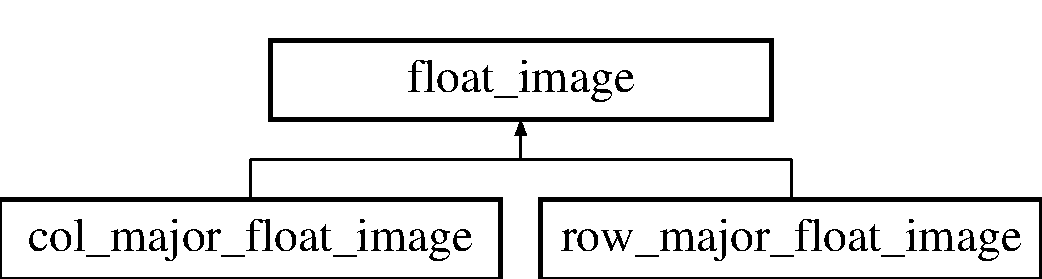
\includegraphics[height=2.000000cm]{classfloat__image}
\end{center}
\end{figure}
\subsection*{Public Member Functions}
\begin{DoxyCompactItemize}
\item 
\hyperlink{classfloat__image_a9e4ea7f98eb8c33e025cd21d61703c66}{float\-\_\-image} (long width, long height)
\item 
\hyperlink{classfloat__image_a4626247e8da835a5be04e346b577f85e}{float\-\_\-image} (float $\ast$data, long width, long height)
\item 
virtual long \hyperlink{classfloat__image_a08ba5e995f656dfebc5aaad0a9be390c}{get\-\_\-width} () const 
\item 
virtual long \hyperlink{classfloat__image_aeab41642909a0ee8d6e0ffcc2e7287b1}{get\-\_\-height} () const 
\item 
virtual float $\ast$ \hyperlink{classfloat__image_ab6dbf1f20614ba84f7b8f2c01b7aa3da}{get\-\_\-data\-\_\-pointer} ()
\item 
virtual float \& \hyperlink{classfloat__image_a62e1446efb51fadcfeebf50568f9d1e9}{operator()} (long w, long h)=0
\item 
\hypertarget{classfloat__image_ae3ae19180d1903bdeb0ffdb6f509a9f5}{virtual float {\bfseries operator()} (long w, long h) const =0}\label{classfloat__image_ae3ae19180d1903bdeb0ffdb6f509a9f5}

\item 
virtual void \hyperlink{classfloat__image_adffd8782a04ea4d764865aace1e43c93}{zero\-\_\-fill} ()
\item 
virtual bool \hyperlink{classfloat__image_a9cead12d50823ca313f6b7b16a57b092}{copy\-\_\-data\-\_\-to} (\hyperlink{classfloat__image}{float\-\_\-image} $\ast$img)
\item 
virtual void \hyperlink{classfloat__image_a3ef2df1d69f6791d2bef54636b625f82}{clear\-\_\-mem} ()
\item 
virtual float \hyperlink{classfloat__image_a53701b38abc94f8a707e8ceb2e6e71da}{get\-\_\-pixel} (long iw, long ih)
\item 
virtual void \hyperlink{classfloat__image_a97b520fc634fc4eb1930491b74d1f79b}{set\-\_\-pixel} (long iw, long ih, float val)
\end{DoxyCompactItemize}
\subsection*{Protected Attributes}
\begin{DoxyCompactItemize}
\item 
\hypertarget{classfloat__image_a43df6eebb483b16921cee23e80f61f5b}{float $\ast$ {\bfseries data}}\label{classfloat__image_a43df6eebb483b16921cee23e80f61f5b}

\item 
\hypertarget{classfloat__image_a92e539199f8cfa3c8ece64e2bdca54c7}{long {\bfseries width}}\label{classfloat__image_a92e539199f8cfa3c8ece64e2bdca54c7}

\item 
\hypertarget{classfloat__image_af7c859a1a77e6886adff0fd47976d069}{long {\bfseries height}}\label{classfloat__image_af7c859a1a77e6886adff0fd47976d069}

\end{DoxyCompactItemize}


\subsection{Detailed Description}
speichert ein 2\-D Bild, welches in einem 1\-D Datenvektor gespeichert wird. Die Ordnung des Datenvektors gibt die Klasse nicht vor. Es müssen auch nicht alle Daten hintereinander weg liegen. Die Zugriffsoperatoren sollen überladen werden, um eine bestimmte Art der Speicherung (z.\-b. row-\/major / column-\/major) oder sonstwas zu abstrahieren. Wichtig\-: Beim Aufruf des Destruktors des Bildes wird das entsprechende Array nicht freigegeben! 

\subsection{Constructor \& Destructor Documentation}
\hypertarget{classfloat__image_a9e4ea7f98eb8c33e025cd21d61703c66}{\index{float\-\_\-image@{float\-\_\-image}!float\-\_\-image@{float\-\_\-image}}
\index{float\-\_\-image@{float\-\_\-image}!float_image@{float\-\_\-image}}
\subsubsection[{float\-\_\-image}]{\setlength{\rightskip}{0pt plus 5cm}float\-\_\-image\-::float\-\_\-image (
\begin{DoxyParamCaption}
\item[{long}]{width, }
\item[{long}]{height}
\end{DoxyParamCaption}
)}}\label{classfloat__image_a9e4ea7f98eb8c33e025cd21d61703c66}
Create float image with and allocate data array! The data will not be zero filled. 
\begin{DoxyParams}{Parameters}
{\em width} & \\
\hline
{\em height} & \\
\hline
\end{DoxyParams}
\hypertarget{classfloat__image_a4626247e8da835a5be04e346b577f85e}{\index{float\-\_\-image@{float\-\_\-image}!float\-\_\-image@{float\-\_\-image}}
\index{float\-\_\-image@{float\-\_\-image}!float_image@{float\-\_\-image}}
\subsubsection[{float\-\_\-image}]{\setlength{\rightskip}{0pt plus 5cm}float\-\_\-image\-::float\-\_\-image (
\begin{DoxyParamCaption}
\item[{float $\ast$}]{data, }
\item[{long}]{width, }
\item[{long}]{height}
\end{DoxyParamCaption}
)}}\label{classfloat__image_a4626247e8da835a5be04e346b577f85e}
Create float image with specified data array. The image will operate on this array. 
\begin{DoxyParams}{Parameters}
{\em data} & \\
\hline
{\em width} & \\
\hline
{\em height} & \\
\hline
\end{DoxyParams}


\subsection{Member Function Documentation}
\hypertarget{classfloat__image_a3ef2df1d69f6791d2bef54636b625f82}{\index{float\-\_\-image@{float\-\_\-image}!clear\-\_\-mem@{clear\-\_\-mem}}
\index{clear\-\_\-mem@{clear\-\_\-mem}!float_image@{float\-\_\-image}}
\subsubsection[{clear\-\_\-mem}]{\setlength{\rightskip}{0pt plus 5cm}void float\-\_\-image\-::clear\-\_\-mem (
\begin{DoxyParamCaption}
{}
\end{DoxyParamCaption}
)\hspace{0.3cm}{\ttfamily [virtual]}}}\label{classfloat__image_a3ef2df1d69f6791d2bef54636b625f82}
Free memory associated with the image. This is not done when the destructor is called. \hypertarget{classfloat__image_a9cead12d50823ca313f6b7b16a57b092}{\index{float\-\_\-image@{float\-\_\-image}!copy\-\_\-data\-\_\-to@{copy\-\_\-data\-\_\-to}}
\index{copy\-\_\-data\-\_\-to@{copy\-\_\-data\-\_\-to}!float_image@{float\-\_\-image}}
\subsubsection[{copy\-\_\-data\-\_\-to}]{\setlength{\rightskip}{0pt plus 5cm}bool float\-\_\-image\-::copy\-\_\-data\-\_\-to (
\begin{DoxyParamCaption}
\item[{{\bf float\-\_\-image} $\ast$}]{img}
\end{DoxyParamCaption}
)\hspace{0.3cm}{\ttfamily [virtual]}}}\label{classfloat__image_a9cead12d50823ca313f6b7b16a57b092}
Copies the data from this image into the given image. Both images need to have the same dimensions. 
\begin{DoxyParams}{Parameters}
{\em img} & Data from this image is copied into img. \\
\hline
\end{DoxyParams}
\begin{DoxyReturn}{Returns}
true if successful, false if not. 
\end{DoxyReturn}
\hypertarget{classfloat__image_ab6dbf1f20614ba84f7b8f2c01b7aa3da}{\index{float\-\_\-image@{float\-\_\-image}!get\-\_\-data\-\_\-pointer@{get\-\_\-data\-\_\-pointer}}
\index{get\-\_\-data\-\_\-pointer@{get\-\_\-data\-\_\-pointer}!float_image@{float\-\_\-image}}
\subsubsection[{get\-\_\-data\-\_\-pointer}]{\setlength{\rightskip}{0pt plus 5cm}float $\ast$ float\-\_\-image\-::get\-\_\-data\-\_\-pointer (
\begin{DoxyParamCaption}
{}
\end{DoxyParamCaption}
)\hspace{0.3cm}{\ttfamily [virtual]}}}\label{classfloat__image_ab6dbf1f20614ba84f7b8f2c01b7aa3da}
\begin{DoxyReturn}{Returns}
pointer to data array 
\end{DoxyReturn}
\hypertarget{classfloat__image_aeab41642909a0ee8d6e0ffcc2e7287b1}{\index{float\-\_\-image@{float\-\_\-image}!get\-\_\-height@{get\-\_\-height}}
\index{get\-\_\-height@{get\-\_\-height}!float_image@{float\-\_\-image}}
\subsubsection[{get\-\_\-height}]{\setlength{\rightskip}{0pt plus 5cm}long float\-\_\-image\-::get\-\_\-height (
\begin{DoxyParamCaption}
{}
\end{DoxyParamCaption}
) const\hspace{0.3cm}{\ttfamily [virtual]}}}\label{classfloat__image_aeab41642909a0ee8d6e0ffcc2e7287b1}
\begin{DoxyReturn}{Returns}
image height 
\end{DoxyReturn}
\hypertarget{classfloat__image_a53701b38abc94f8a707e8ceb2e6e71da}{\index{float\-\_\-image@{float\-\_\-image}!get\-\_\-pixel@{get\-\_\-pixel}}
\index{get\-\_\-pixel@{get\-\_\-pixel}!float_image@{float\-\_\-image}}
\subsubsection[{get\-\_\-pixel}]{\setlength{\rightskip}{0pt plus 5cm}float float\-\_\-image\-::get\-\_\-pixel (
\begin{DoxyParamCaption}
\item[{long}]{iw, }
\item[{long}]{ih}
\end{DoxyParamCaption}
)\hspace{0.3cm}{\ttfamily [virtual]}}}\label{classfloat__image_a53701b38abc94f8a707e8ceb2e6e71da}
Get Pixel value at specified position. 
\begin{DoxyParams}{Parameters}
{\em iw} & \\
\hline
{\em ih} & \\
\hline
\end{DoxyParams}
\begin{DoxyReturn}{Returns}

\end{DoxyReturn}
\hypertarget{classfloat__image_a08ba5e995f656dfebc5aaad0a9be390c}{\index{float\-\_\-image@{float\-\_\-image}!get\-\_\-width@{get\-\_\-width}}
\index{get\-\_\-width@{get\-\_\-width}!float_image@{float\-\_\-image}}
\subsubsection[{get\-\_\-width}]{\setlength{\rightskip}{0pt plus 5cm}long float\-\_\-image\-::get\-\_\-width (
\begin{DoxyParamCaption}
{}
\end{DoxyParamCaption}
) const\hspace{0.3cm}{\ttfamily [virtual]}}}\label{classfloat__image_a08ba5e995f656dfebc5aaad0a9be390c}
\begin{DoxyReturn}{Returns}
image width 
\end{DoxyReturn}
\hypertarget{classfloat__image_a62e1446efb51fadcfeebf50568f9d1e9}{\index{float\-\_\-image@{float\-\_\-image}!operator()@{operator()}}
\index{operator()@{operator()}!float_image@{float\-\_\-image}}
\subsubsection[{operator()}]{\setlength{\rightskip}{0pt plus 5cm}virtual float\& float\-\_\-image\-::operator() (
\begin{DoxyParamCaption}
\item[{long}]{w, }
\item[{long}]{h}
\end{DoxyParamCaption}
)\hspace{0.3cm}{\ttfamily [pure virtual]}}}\label{classfloat__image_a62e1446efb51fadcfeebf50568f9d1e9}
Return element at position width = w, height = h, starting with (0,0) in upper left corner of the image. Implemented in child classes, see e.\-g. \hyperlink{classrow__major__float__image}{row\-\_\-major\-\_\-float\-\_\-image}. 

Implemented in \hyperlink{classcol__major__float__image_a45315790d78a3d27559946f198129708}{col\-\_\-major\-\_\-float\-\_\-image}, and \hyperlink{classrow__major__float__image_a04b9b253a3771e0963c839a9a85ccd99}{row\-\_\-major\-\_\-float\-\_\-image}.

\hypertarget{classfloat__image_a97b520fc634fc4eb1930491b74d1f79b}{\index{float\-\_\-image@{float\-\_\-image}!set\-\_\-pixel@{set\-\_\-pixel}}
\index{set\-\_\-pixel@{set\-\_\-pixel}!float_image@{float\-\_\-image}}
\subsubsection[{set\-\_\-pixel}]{\setlength{\rightskip}{0pt plus 5cm}void float\-\_\-image\-::set\-\_\-pixel (
\begin{DoxyParamCaption}
\item[{long}]{iw, }
\item[{long}]{ih, }
\item[{float}]{val}
\end{DoxyParamCaption}
)\hspace{0.3cm}{\ttfamily [virtual]}}}\label{classfloat__image_a97b520fc634fc4eb1930491b74d1f79b}
Set Pixel value at specified position. 
\begin{DoxyParams}{Parameters}
{\em iw} & \\
\hline
{\em ih} & \\
\hline
{\em val} & \\
\hline
\end{DoxyParams}
\begin{DoxyReturn}{Returns}

\end{DoxyReturn}
\hypertarget{classfloat__image_adffd8782a04ea4d764865aace1e43c93}{\index{float\-\_\-image@{float\-\_\-image}!zero\-\_\-fill@{zero\-\_\-fill}}
\index{zero\-\_\-fill@{zero\-\_\-fill}!float_image@{float\-\_\-image}}
\subsubsection[{zero\-\_\-fill}]{\setlength{\rightskip}{0pt plus 5cm}void float\-\_\-image\-::zero\-\_\-fill (
\begin{DoxyParamCaption}
{}
\end{DoxyParamCaption}
)\hspace{0.3cm}{\ttfamily [virtual]}}}\label{classfloat__image_adffd8782a04ea4d764865aace1e43c93}
Fill image with zeroes. 

The documentation for this class was generated from the following files\-:\begin{DoxyCompactItemize}
\item 
include/float\-\_\-image.\-h\item 
src/float\-\_\-image.\-cpp\end{DoxyCompactItemize}

\hypertarget{classgrad__fit__tile__unwrapper}{\section{grad\-\_\-fit\-\_\-tile\-\_\-unwrapper Class Reference}
\label{classgrad__fit__tile__unwrapper}\index{grad\-\_\-fit\-\_\-tile\-\_\-unwrapper@{grad\-\_\-fit\-\_\-tile\-\_\-unwrapper}}
}
Inheritance diagram for grad\-\_\-fit\-\_\-tile\-\_\-unwrapper\-:\begin{figure}[H]
\begin{center}
\leavevmode
\includegraphics[height=2.000000cm]{classgrad__fit__tile__unwrapper}
\end{center}
\end{figure}
\subsection*{Public Member Functions}
\begin{DoxyCompactItemize}
\item 
\hypertarget{classgrad__fit__tile__unwrapper_a79033def7d478d1ef50b627b0663700d}{void {\bfseries unwrap} (sharedptr$<$ \hyperlink{classtile}{tile} $>$ t)}\label{classgrad__fit__tile__unwrapper_a79033def7d478d1ef50b627b0663700d}

\item 
virtual std\-::string \hyperlink{classgrad__fit__tile__unwrapper_a46a71a2adc53411289f792aae8c1b61c}{get\-\_\-name} ()
\item 
virtual void \hyperlink{classgrad__fit__tile__unwrapper_a62df2a6e799306b85f273a4f5aa43b4c}{usage\-\_\-help} ()
\end{DoxyCompactItemize}


\subsection{Member Function Documentation}
\hypertarget{classgrad__fit__tile__unwrapper_a46a71a2adc53411289f792aae8c1b61c}{\index{grad\-\_\-fit\-\_\-tile\-\_\-unwrapper@{grad\-\_\-fit\-\_\-tile\-\_\-unwrapper}!get\-\_\-name@{get\-\_\-name}}
\index{get\-\_\-name@{get\-\_\-name}!grad_fit_tile_unwrapper@{grad\-\_\-fit\-\_\-tile\-\_\-unwrapper}}
\subsubsection[{get\-\_\-name}]{\setlength{\rightskip}{0pt plus 5cm}std\-::string grad\-\_\-fit\-\_\-tile\-\_\-unwrapper\-::get\-\_\-name (
\begin{DoxyParamCaption}
{}
\end{DoxyParamCaption}
)\hspace{0.3cm}{\ttfamily [virtual]}}}\label{classgrad__fit__tile__unwrapper_a46a71a2adc53411289f792aae8c1b61c}
Return a name (with options) to set in the output file name 

Implements \hyperlink{classabstract__tile__unwrapper_ae70f69a703e622e5ab13eabcc91fca4d}{abstract\-\_\-tile\-\_\-unwrapper}.

\hypertarget{classgrad__fit__tile__unwrapper_a62df2a6e799306b85f273a4f5aa43b4c}{\index{grad\-\_\-fit\-\_\-tile\-\_\-unwrapper@{grad\-\_\-fit\-\_\-tile\-\_\-unwrapper}!usage\-\_\-help@{usage\-\_\-help}}
\index{usage\-\_\-help@{usage\-\_\-help}!grad_fit_tile_unwrapper@{grad\-\_\-fit\-\_\-tile\-\_\-unwrapper}}
\subsubsection[{usage\-\_\-help}]{\setlength{\rightskip}{0pt plus 5cm}void grad\-\_\-fit\-\_\-tile\-\_\-unwrapper\-::usage\-\_\-help (
\begin{DoxyParamCaption}
{}
\end{DoxyParamCaption}
)\hspace{0.3cm}{\ttfamily [virtual]}}}\label{classgrad__fit__tile__unwrapper_a62df2a6e799306b85f273a4f5aa43b4c}
Display a help on how to use this merger, in particular usage of merger-\/settings 

Implements \hyperlink{classabstract__tile__unwrapper_a469b36a7f302d5a2655631bbdb6f8daf}{abstract\-\_\-tile\-\_\-unwrapper}.



The documentation for this class was generated from the following files\-:\begin{DoxyCompactItemize}
\item 
include/algorithm/grad\-\_\-fit\-\_\-tile\-\_\-unwrapper.\-h\item 
src/algorithm/grad\-\_\-fit\-\_\-tile\-\_\-unwrapper.\-cpp\end{DoxyCompactItemize}

\hypertarget{classleast__squares__grad__unwrapper}{\section{least\-\_\-squares\-\_\-grad\-\_\-unwrapper Class Reference}
\label{classleast__squares__grad__unwrapper}\index{least\-\_\-squares\-\_\-grad\-\_\-unwrapper@{least\-\_\-squares\-\_\-grad\-\_\-unwrapper}}
}


{\ttfamily \#include $<$least\-\_\-squares\-\_\-grad\-\_\-unwrapper.\-h$>$}

Inheritance diagram for least\-\_\-squares\-\_\-grad\-\_\-unwrapper\-:\begin{figure}[H]
\begin{center}
\leavevmode
\includegraphics[height=2.000000cm]{classleast__squares__grad__unwrapper}
\end{center}
\end{figure}
\subsection*{Public Member Functions}
\begin{DoxyCompactItemize}
\item 
\hyperlink{classleast__squares__grad__unwrapper_a33a10b9f3200e5b1fb5827dc50687772}{least\-\_\-squares\-\_\-grad\-\_\-unwrapper} (std\-::vector$<$ std\-::string $>$ usettings)
\item 
\hyperlink{classleast__squares__grad__unwrapper_ab22c6e1009b5b8ceae4dea542d0f469d}{least\-\_\-squares\-\_\-grad\-\_\-unwrapper} (sharedptr$<$ \hyperlink{classmodel__function}{model\-\_\-function} $>$ model)
\item 
\hypertarget{classleast__squares__grad__unwrapper_ab7a1685800926ffbba4b1e829a21052d}{virtual \hyperlink{classleast__squares__grad__unwrapper_ab7a1685800926ffbba4b1e829a21052d}{$\sim$least\-\_\-squares\-\_\-grad\-\_\-unwrapper} ()}\label{classleast__squares__grad__unwrapper_ab7a1685800926ffbba4b1e829a21052d}

\begin{DoxyCompactList}\small\item\em Destructor. \end{DoxyCompactList}\item 
void \hyperlink{classleast__squares__grad__unwrapper_a4a0c29f7e7cfa21b5a87a291565d123f}{unwrap} (sharedptr$<$ \hyperlink{classtile}{tile} $>$ t)
\item 
virtual std\-::string \hyperlink{classleast__squares__grad__unwrapper_af66d1a659d6cfbb82200d120f43dd939}{get\-\_\-name} ()
\item 
virtual void \hyperlink{classleast__squares__grad__unwrapper_a8795b4b968a336d28a81e910cbc9f4ab}{usage\-\_\-help} ()
\end{DoxyCompactItemize}


\subsection{Detailed Description}
This class uses a general linear least squares approach for unwrapping the tiles (M\-L\-S\-Q\-U). General\-: Within its constructor, this class takes a given set of base functions, calculates the coefficients and fit them to the data. Linear\-: The choice of the base functions is up to the user. Only limitation is that these base functions have to be linear in the coefficients. Eg. a$\ast$x$^\wedge$5$\ast$y$^\wedge$3, b$\ast$x$^\wedge$2, c$\ast$1 is as good as a$\ast$sin(x), b$\ast$cos(x/4), c$\ast$tan(3). N\-O\-T working is sin(a$\ast$x), x$^\wedge$b, x$^\wedge$y. Least Squares\-: This approach leads to a big matrix / system of equastions, which will be solved with least squares methods, namely the S\-V-\/\-Decomposition.

This class will always use the second order gradient calculator for calculation of the gradient profile of the tile. Thus it will always operate on a \hyperlink{classunit__cartesian__coordinate__system}{unit\-\_\-cartesian\-\_\-coordinate\-\_\-system} 

\subsection{Constructor \& Destructor Documentation}
\hypertarget{classleast__squares__grad__unwrapper_a33a10b9f3200e5b1fb5827dc50687772}{\index{least\-\_\-squares\-\_\-grad\-\_\-unwrapper@{least\-\_\-squares\-\_\-grad\-\_\-unwrapper}!least\-\_\-squares\-\_\-grad\-\_\-unwrapper@{least\-\_\-squares\-\_\-grad\-\_\-unwrapper}}
\index{least\-\_\-squares\-\_\-grad\-\_\-unwrapper@{least\-\_\-squares\-\_\-grad\-\_\-unwrapper}!least_squares_grad_unwrapper@{least\-\_\-squares\-\_\-grad\-\_\-unwrapper}}
\subsubsection[{least\-\_\-squares\-\_\-grad\-\_\-unwrapper}]{\setlength{\rightskip}{0pt plus 5cm}least\-\_\-squares\-\_\-grad\-\_\-unwrapper\-::least\-\_\-squares\-\_\-grad\-\_\-unwrapper (
\begin{DoxyParamCaption}
\item[{std\-::vector$<$ std\-::string $>$}]{usettings}
\end{DoxyParamCaption}
)}}\label{classleast__squares__grad__unwrapper_a33a10b9f3200e5b1fb5827dc50687772}
This constructor is used in the main programm working with the command line option. 
\begin{DoxyParams}{Parameters}
{\em usettings} & vector of strings with options for the unwrapper \\
\hline
\end{DoxyParams}
\hypertarget{classleast__squares__grad__unwrapper_ab22c6e1009b5b8ceae4dea542d0f469d}{\index{least\-\_\-squares\-\_\-grad\-\_\-unwrapper@{least\-\_\-squares\-\_\-grad\-\_\-unwrapper}!least\-\_\-squares\-\_\-grad\-\_\-unwrapper@{least\-\_\-squares\-\_\-grad\-\_\-unwrapper}}
\index{least\-\_\-squares\-\_\-grad\-\_\-unwrapper@{least\-\_\-squares\-\_\-grad\-\_\-unwrapper}!least_squares_grad_unwrapper@{least\-\_\-squares\-\_\-grad\-\_\-unwrapper}}
\subsubsection[{least\-\_\-squares\-\_\-grad\-\_\-unwrapper}]{\setlength{\rightskip}{0pt plus 5cm}least\-\_\-squares\-\_\-grad\-\_\-unwrapper\-::least\-\_\-squares\-\_\-grad\-\_\-unwrapper (
\begin{DoxyParamCaption}
\item[{sharedptr$<$ {\bf model\-\_\-function} $>$}]{model}
\end{DoxyParamCaption}
)}}\label{classleast__squares__grad__unwrapper_ab22c6e1009b5b8ceae4dea542d0f469d}
Constructor with explicit model function as a parameter 

\subsection{Member Function Documentation}
\hypertarget{classleast__squares__grad__unwrapper_af66d1a659d6cfbb82200d120f43dd939}{\index{least\-\_\-squares\-\_\-grad\-\_\-unwrapper@{least\-\_\-squares\-\_\-grad\-\_\-unwrapper}!get\-\_\-name@{get\-\_\-name}}
\index{get\-\_\-name@{get\-\_\-name}!least_squares_grad_unwrapper@{least\-\_\-squares\-\_\-grad\-\_\-unwrapper}}
\subsubsection[{get\-\_\-name}]{\setlength{\rightskip}{0pt plus 5cm}std\-::string least\-\_\-squares\-\_\-grad\-\_\-unwrapper\-::get\-\_\-name (
\begin{DoxyParamCaption}
{}
\end{DoxyParamCaption}
)\hspace{0.3cm}{\ttfamily [virtual]}}}\label{classleast__squares__grad__unwrapper_af66d1a659d6cfbb82200d120f43dd939}
Return a name (with options) to set in the output file name 

Implements \hyperlink{classabstract__tile__unwrapper_ae70f69a703e622e5ab13eabcc91fca4d}{abstract\-\_\-tile\-\_\-unwrapper}.

\hypertarget{classleast__squares__grad__unwrapper_a4a0c29f7e7cfa21b5a87a291565d123f}{\index{least\-\_\-squares\-\_\-grad\-\_\-unwrapper@{least\-\_\-squares\-\_\-grad\-\_\-unwrapper}!unwrap@{unwrap}}
\index{unwrap@{unwrap}!least_squares_grad_unwrapper@{least\-\_\-squares\-\_\-grad\-\_\-unwrapper}}
\subsubsection[{unwrap}]{\setlength{\rightskip}{0pt plus 5cm}void least\-\_\-squares\-\_\-grad\-\_\-unwrapper\-::unwrap (
\begin{DoxyParamCaption}
\item[{sharedptr$<$ {\bf tile} $>$}]{t}
\end{DoxyParamCaption}
)}}\label{classleast__squares__grad__unwrapper_a4a0c29f7e7cfa21b5a87a291565d123f}
Unwrap a given tile. 
\begin{DoxyParams}{Parameters}
{\em t} & \\
\hline
\end{DoxyParams}
sharedptr$<$abstr....\-unwrapper$>$ stu this-\/$>$model-\/$>$subtract\-\_\-wrap\-\_\-add\-\_\-function(t, sharedptr$<$abstract\-\_\-tile\-\_\-unwrapper$>$ strand\-\_\-bla);\hypertarget{classleast__squares__grad__unwrapper_a8795b4b968a336d28a81e910cbc9f4ab}{\index{least\-\_\-squares\-\_\-grad\-\_\-unwrapper@{least\-\_\-squares\-\_\-grad\-\_\-unwrapper}!usage\-\_\-help@{usage\-\_\-help}}
\index{usage\-\_\-help@{usage\-\_\-help}!least_squares_grad_unwrapper@{least\-\_\-squares\-\_\-grad\-\_\-unwrapper}}
\subsubsection[{usage\-\_\-help}]{\setlength{\rightskip}{0pt plus 5cm}void least\-\_\-squares\-\_\-grad\-\_\-unwrapper\-::usage\-\_\-help (
\begin{DoxyParamCaption}
{}
\end{DoxyParamCaption}
)\hspace{0.3cm}{\ttfamily [virtual]}}}\label{classleast__squares__grad__unwrapper_a8795b4b968a336d28a81e910cbc9f4ab}
Display a help on how to use this merger, in particular usage of merger-\/settings 

Implements \hyperlink{classabstract__tile__unwrapper_a469b36a7f302d5a2655631bbdb6f8daf}{abstract\-\_\-tile\-\_\-unwrapper}.



The documentation for this class was generated from the following files\-:\begin{DoxyCompactItemize}
\item 
include/algorithm/least\-\_\-squares\-\_\-grad\-\_\-unwrapper.\-h\item 
src/algorithm/least\-\_\-squares\-\_\-grad\-\_\-unwrapper.\-cpp\end{DoxyCompactItemize}

\hypertarget{classmeasure__pixel__energy}{\section{measure\-\_\-pixel\-\_\-energy Class Reference}
\label{classmeasure__pixel__energy}\index{measure\-\_\-pixel\-\_\-energy@{measure\-\_\-pixel\-\_\-energy}}
}


{\ttfamily \#include $<$measure\-\_\-pixel\-\_\-energy.\-h$>$}

\subsection*{Public Member Functions}
\begin{DoxyCompactItemize}
\item 
\hypertarget{classmeasure__pixel__energy_aa9963e55dd7af85c1935775973c75975}{\hyperlink{classmeasure__pixel__energy_aa9963e55dd7af85c1935775973c75975}{measure\-\_\-pixel\-\_\-energy} ()}\label{classmeasure__pixel__energy_aa9963e55dd7af85c1935775973c75975}

\begin{DoxyCompactList}\small\item\em Std constructor. \end{DoxyCompactList}\item 
\hypertarget{classmeasure__pixel__energy_aa363a45d7c89bd76509b384d0597cfb8}{virtual \hyperlink{classmeasure__pixel__energy_aa363a45d7c89bd76509b384d0597cfb8}{$\sim$measure\-\_\-pixel\-\_\-energy} ()}\label{classmeasure__pixel__energy_aa363a45d7c89bd76509b384d0597cfb8}

\begin{DoxyCompactList}\small\item\em Destructor. \end{DoxyCompactList}\item 
float \hyperlink{classmeasure__pixel__energy_af74ec0c136a474c85102a292c157a5a9}{calc} (sharedptr$<$ \hyperlink{classrow__major__float__image}{row\-\_\-major\-\_\-float\-\_\-image} $>$ image)
\end{DoxyCompactItemize}


\subsection{Detailed Description}
This class provides a measure of the quality for a image provided. The quality is set to the summation over every neighbouring tiles squared difference. Therefore faulty unwraps result in a big penalty, increasing the \char`\"{}energy\char`\"{} of the image. Note\-: This measure is not definite, it only provides a option to compare two familiar images. E.\-g. compare a image unwrapped with unwrapper\#1 and the same image unwarpped with unwrapper\#2. 

\subsection{Member Function Documentation}
\hypertarget{classmeasure__pixel__energy_af74ec0c136a474c85102a292c157a5a9}{\index{measure\-\_\-pixel\-\_\-energy@{measure\-\_\-pixel\-\_\-energy}!calc@{calc}}
\index{calc@{calc}!measure_pixel_energy@{measure\-\_\-pixel\-\_\-energy}}
\subsubsection[{calc}]{\setlength{\rightskip}{0pt plus 5cm}float measure\-\_\-pixel\-\_\-energy\-::calc (
\begin{DoxyParamCaption}
\item[{sharedptr$<$ {\bf row\-\_\-major\-\_\-float\-\_\-image} $>$}]{image}
\end{DoxyParamCaption}
)}}\label{classmeasure__pixel__energy_af74ec0c136a474c85102a292c157a5a9}
This method calculates the energy of the image 
\begin{DoxyParams}{Parameters}
{\em image} & the image \\
\hline
\end{DoxyParams}
\begin{DoxyReturn}{Returns}
energy-\/value 
\end{DoxyReturn}


The documentation for this class was generated from the following files\-:\begin{DoxyCompactItemize}
\item 
include/analyse/measure\-\_\-pixel\-\_\-energy.\-h\item 
src/analyse/measure\-\_\-pixel\-\_\-energy.\-cpp\end{DoxyCompactItemize}

\hypertarget{classmeasure__psnr}{\section{measure\-\_\-psnr Class Reference}
\label{classmeasure__psnr}\index{measure\-\_\-psnr@{measure\-\_\-psnr}}
}
\subsection*{Public Member Functions}
\begin{DoxyCompactItemize}
\item 
\hyperlink{classmeasure__psnr_a907c9fd1dcaf8a3bd7a41c6efbedff17}{measure\-\_\-psnr} (sharedptr$<$ \hyperlink{classrow__major__float__image}{row\-\_\-major\-\_\-float\-\_\-image} $>$ noisy\-\_\-img, sharedptr$<$ \hyperlink{classrow__major__float__image}{row\-\_\-major\-\_\-float\-\_\-image} $>$ orig\-\_\-img, int bit)
\item 
float \hyperlink{classmeasure__psnr_a64f7e3b05beefa9a8345c78fe2add744}{calculate\-\_\-psnr} ()
\end{DoxyCompactItemize}


\subsection{Constructor \& Destructor Documentation}
\hypertarget{classmeasure__psnr_a907c9fd1dcaf8a3bd7a41c6efbedff17}{\index{measure\-\_\-psnr@{measure\-\_\-psnr}!measure\-\_\-psnr@{measure\-\_\-psnr}}
\index{measure\-\_\-psnr@{measure\-\_\-psnr}!measure_psnr@{measure\-\_\-psnr}}
\subsubsection[{measure\-\_\-psnr}]{\setlength{\rightskip}{0pt plus 5cm}measure\-\_\-psnr\-::measure\-\_\-psnr (
\begin{DoxyParamCaption}
\item[{sharedptr$<$ {\bf row\-\_\-major\-\_\-float\-\_\-image} $>$}]{noisy\-\_\-img, }
\item[{sharedptr$<$ {\bf row\-\_\-major\-\_\-float\-\_\-image} $>$}]{orig\-\_\-img, }
\item[{int}]{bit}
\end{DoxyParamCaption}
)}}\label{classmeasure__psnr_a907c9fd1dcaf8a3bd7a41c6efbedff17}
Constructor 
\begin{DoxyParams}{Parameters}
{\em noisy\-\_\-img} & picture with noise \\
\hline
{\em orig\-\_\-img} & picture without noise \\
\hline
{\em bit} & \#bit the images have \\
\hline
\end{DoxyParams}


\subsection{Member Function Documentation}
\hypertarget{classmeasure__psnr_a64f7e3b05beefa9a8345c78fe2add744}{\index{measure\-\_\-psnr@{measure\-\_\-psnr}!calculate\-\_\-psnr@{calculate\-\_\-psnr}}
\index{calculate\-\_\-psnr@{calculate\-\_\-psnr}!measure_psnr@{measure\-\_\-psnr}}
\subsubsection[{calculate\-\_\-psnr}]{\setlength{\rightskip}{0pt plus 5cm}float measure\-\_\-psnr\-::calculate\-\_\-psnr (
\begin{DoxyParamCaption}
{}
\end{DoxyParamCaption}
)}}\label{classmeasure__psnr_a64f7e3b05beefa9a8345c78fe2add744}
Calculates and returns the psnr of the given image \begin{DoxyReturn}{Returns}
psnr 
\end{DoxyReturn}


The documentation for this class was generated from the following files\-:\begin{DoxyCompactItemize}
\item 
include/analyse/measure\-\_\-psnr.\-h\item 
src/analyse/measure\-\_\-psnr.\-cpp\end{DoxyCompactItemize}

\hypertarget{classmodel__function}{\section{model\-\_\-function Class Reference}
\label{classmodel__function}\index{model\-\_\-function@{model\-\_\-function}}
}


{\ttfamily \#include $<$model\-\_\-function.\-h$>$}

Inheritance diagram for model\-\_\-function\-:\begin{figure}[H]
\begin{center}
\leavevmode
\includegraphics[height=2.000000cm]{classmodel__function}
\end{center}
\end{figure}
\subsection*{Public Member Functions}
\begin{DoxyCompactItemize}
\item 
\hypertarget{classmodel__function_a1a982c2cec5a63de6c1480e0b1c946eb}{\hyperlink{classmodel__function_a1a982c2cec5a63de6c1480e0b1c946eb}{model\-\_\-function} ()}\label{classmodel__function_a1a982c2cec5a63de6c1480e0b1c946eb}

\begin{DoxyCompactList}\small\item\em Std constructor. \end{DoxyCompactList}\item 
\hyperlink{classmodel__function_a2e9d9ebb47826758798b094079f1abcc}{model\-\_\-function} (sharedptr$<$ std\-::vector$<$ sharedptr$<$ \hyperlink{classabstract__function}{abstract\-\_\-function} $>$ $>$ $>$ vc\-\_\-base, sharedptr$<$ \hyperlink{classabstract__coordinate__system}{abstract\-\_\-coordinate\-\_\-system} $>$ coord\-\_\-system)
\item 
\hypertarget{classmodel__function_a9f51895f06daf4d454b16eccf44dc57c}{virtual \hyperlink{classmodel__function_a9f51895f06daf4d454b16eccf44dc57c}{$\sim$model\-\_\-function} ()}\label{classmodel__function_a9f51895f06daf4d454b16eccf44dc57c}

\begin{DoxyCompactList}\small\item\em Destruktor. \end{DoxyCompactList}\item 
float \hyperlink{classmodel__function_a5ca38b00e9064eb46b697dab3b3e848f}{eval} (float x, float y)
\item 
float \hyperlink{classmodel__function_add97095253744605c1da638d2dc6c3b0}{eval} (float x, float y, sharedptr$<$ std\-::vector$<$ float $>$ $>$ vc\-\_\-coeff)
\item 
float \hyperlink{classmodel__function_a2f5c7afd1f910bef7f545c0384a23c1e}{eval} (float x, float y, sharedptr$<$ Eigen\-::\-Vector\-Xf $>$ v\-\_\-coeff)
\item 
sharedptr$<$ \hyperlink{classabstract__gradient}{abstract\-\_\-gradient} $>$ \hyperlink{classmodel__function_adf3a7a6ff204c7e993f63f61cd2cfcf1}{get\-\_\-gradient} ()
\item 
\hypertarget{classmodel__function_a0e4bcd2cf988b0e9f06d25f9ef552d71}{sharedptr\\*
$<$ \hyperlink{classabstract__coordinate__system}{abstract\-\_\-coordinate\-\_\-system} $>$ \hyperlink{classmodel__function_a0e4bcd2cf988b0e9f06d25f9ef552d71}{get\-\_\-coordinate\-\_\-system} ()}\label{classmodel__function_a0e4bcd2cf988b0e9f06d25f9ef552d71}

\begin{DoxyCompactList}\small\item\em Returs a pointer to the used coordinate system. This is the unit cartesian system given by the \hyperlink{classsecond__order__gradient}{second\-\_\-order\-\_\-gradient} calculator. \end{DoxyCompactList}\item 
void \hyperlink{classmodel__function_ace253fd777dee5695cc0b8b3591e0fc7}{set\-\_\-coeff\-\_\-vector} (sharedptr$<$ std\-::vector$<$ float $>$ $>$ coeff)
\item 
\hypertarget{classmodel__function_ad83f4720b10229ae6369a85bc9606bdf}{void \hyperlink{classmodel__function_ad83f4720b10229ae6369a85bc9606bdf}{set\-\_\-coeff\-\_\-vector} (sharedptr$<$ Eigen\-::\-Vector\-Xf $>$ coeff)}\label{classmodel__function_ad83f4720b10229ae6369a85bc9606bdf}

\begin{DoxyCompactList}\small\item\em Overloaded function to work with Eigen\-::\-Vector\-Xf. \end{DoxyCompactList}\item 
void \hyperlink{classmodel__function_a4064f37008f43c8921c3ca20541eb75c}{set\-\_\-base\-\_\-vector} (sharedptr$<$ std\-::vector$<$ sharedptr$<$ \hyperlink{classabstract__function}{abstract\-\_\-function} $>$ $>$ $>$ vc\-\_\-base)
\item 
\hypertarget{classmodel__function_a776e5515af16cc021e7ff72ad6e10bad}{void \hyperlink{classmodel__function_a776e5515af16cc021e7ff72ad6e10bad}{set\-\_\-constant\-\_\-offset} (float value)}\label{classmodel__function_a776e5515af16cc021e7ff72ad6e10bad}

\begin{DoxyCompactList}\small\item\em Set the constant offset of this function to the specified value. \end{DoxyCompactList}\item 
sharedptr$<$ std\-::vector\\*
$<$ sharedptr$<$ \hyperlink{classabstract__function}{abstract\-\_\-function} $>$ $>$ $>$ \hyperlink{classmodel__function_a6c3b24ae19c7178775002a5178487f9e}{get\-\_\-base\-\_\-vector} ()
\item 
int \hyperlink{classmodel__function_a9af5216fc0b4964b4269ff4babee4c4d}{get\-\_\-coeff\-\_\-size} ()
\item 
int \hyperlink{classmodel__function_acfbb42766697bfc2dcaeb045e5ab60d0}{get\-\_\-base\-\_\-size} ()
\item 
\hypertarget{classmodel__function_abad3b2aa7dab1fe6cb7e657166a608dc}{float \hyperlink{classmodel__function_abad3b2aa7dab1fe6cb7e657166a608dc}{get\-\_\-constant\-\_\-offset} ()}\label{classmodel__function_abad3b2aa7dab1fe6cb7e657166a608dc}

\begin{DoxyCompactList}\small\item\em Return the constant offset of this function. \end{DoxyCompactList}\item 
void \hyperlink{classmodel__function_a16243e1bb23590acce533652d6eed732}{subtract\-\_\-wrap\-\_\-add\-\_\-function} (sharedptr$<$ \hyperlink{classtile}{tile} $>$ t, int step\-\_\-count)
\end{DoxyCompactItemize}
\subsection*{Protected Attributes}
\begin{DoxyCompactItemize}
\item 
\hypertarget{classmodel__function_ac27dd96bd16703d8015997a0e9011a33}{sharedptr\\*
$<$ \hyperlink{classabstract__coordinate__system}{abstract\-\_\-coordinate\-\_\-system} $>$ \hyperlink{classmodel__function_ac27dd96bd16703d8015997a0e9011a33}{coordinate\-\_\-system}}\label{classmodel__function_ac27dd96bd16703d8015997a0e9011a33}

\begin{DoxyCompactList}\small\item\em The model functions holds the coordinate system used. \end{DoxyCompactList}\end{DoxyCompactItemize}


\subsection{Detailed Description}
This class implements a vector of base functions. These are linear combined to a full function, providing a method to model the image with functions. Major advantage is that the functions itself must not be linear, nor be constants. Polynomial functions as well as a linear combination of exponentiation of sin/cosin. !! Base functions must not be constants. A constant offset is treated separately by the model function. It is set to 0 on initialization. 

\subsection{Constructor \& Destructor Documentation}
\hypertarget{classmodel__function_a2e9d9ebb47826758798b094079f1abcc}{\index{model\-\_\-function@{model\-\_\-function}!model\-\_\-function@{model\-\_\-function}}
\index{model\-\_\-function@{model\-\_\-function}!model_function@{model\-\_\-function}}
\subsubsection[{model\-\_\-function}]{\setlength{\rightskip}{0pt plus 5cm}model\-\_\-function\-::model\-\_\-function (
\begin{DoxyParamCaption}
\item[{sharedptr$<$ std\-::vector$<$ sharedptr$<$ {\bf abstract\-\_\-function} $>$ $>$ $>$}]{vc\-\_\-base, }
\item[{sharedptr$<$ {\bf abstract\-\_\-coordinate\-\_\-system} $>$}]{coord\-\_\-system}
\end{DoxyParamCaption}
)}}\label{classmodel__function_a2e9d9ebb47826758798b094079f1abcc}

\begin{DoxyParams}{Parameters}
{\em vc\-\_\-base} & vector of base functions this method should use \\
\hline
{\em coord\-\_\-system} & coordinate system in use with this base functions \\
\hline
\end{DoxyParams}


\subsection{Member Function Documentation}
\hypertarget{classmodel__function_a5ca38b00e9064eb46b697dab3b3e848f}{\index{model\-\_\-function@{model\-\_\-function}!eval@{eval}}
\index{eval@{eval}!model_function@{model\-\_\-function}}
\subsubsection[{eval}]{\setlength{\rightskip}{0pt plus 5cm}float model\-\_\-function\-::eval (
\begin{DoxyParamCaption}
\item[{float}]{x, }
\item[{float}]{y}
\end{DoxyParamCaption}
)\hspace{0.3cm}{\ttfamily [virtual]}}}\label{classmodel__function_a5ca38b00e9064eb46b697dab3b3e848f}
Evaluates the value of this function with the coefficients this model itself holds 
\begin{DoxyParams}{Parameters}
{\em x} & coordinate \\
\hline
{\em y} & coordinate \\
\hline
\end{DoxyParams}
\begin{DoxyReturn}{Returns}
value of this function
\end{DoxyReturn}
Calculate the value of this function with \char`\"{}build-\/in\char`\"{} coefficients. 
\begin{DoxyParams}{Parameters}
{\em x} & coordinate \\
\hline
{\em y} & coordinate \\
\hline
\end{DoxyParams}
\begin{DoxyReturn}{Returns}
value of the function 
\end{DoxyReturn}


Implements \hyperlink{classabstract__function_ae313a63bae0ae1b88bcabd1bebc22f4f}{abstract\-\_\-function}.

\hypertarget{classmodel__function_add97095253744605c1da638d2dc6c3b0}{\index{model\-\_\-function@{model\-\_\-function}!eval@{eval}}
\index{eval@{eval}!model_function@{model\-\_\-function}}
\subsubsection[{eval}]{\setlength{\rightskip}{0pt plus 5cm}float model\-\_\-function\-::eval (
\begin{DoxyParamCaption}
\item[{float}]{x, }
\item[{float}]{y, }
\item[{sharedptr$<$ std\-::vector$<$ float $>$ $>$}]{vc\-\_\-coeff}
\end{DoxyParamCaption}
)}}\label{classmodel__function_add97095253744605c1da638d2dc6c3b0}
Evaluates the value of this function with the coefficients provided 
\begin{DoxyParams}{Parameters}
{\em x} & coordinate \\
\hline
{\em y} & coordinate \\
\hline
{\em vc\-\_\-coeff} & set of coeff to scale the base functions. N\-O\-T\-E\-: Must have the same size as the base functions... \\
\hline
\end{DoxyParams}
\begin{DoxyReturn}{Returns}
value of this function
\end{DoxyReturn}
Calculate the value of this function. 
\begin{DoxyParams}{Parameters}
{\em x} & coordinate \\
\hline
{\em y} & coordinate \\
\hline
{\em vc\-\_\-coeff} & set of coefficients for the linear combination of the base functions. N\-O\-T\-E\-: vc\-\_\-coeff must have the same amount of elements as there are base functions. \\
\hline
\end{DoxyParams}
\begin{DoxyReturn}{Returns}
value of the function 
\end{DoxyReturn}
\hypertarget{classmodel__function_a2f5c7afd1f910bef7f545c0384a23c1e}{\index{model\-\_\-function@{model\-\_\-function}!eval@{eval}}
\index{eval@{eval}!model_function@{model\-\_\-function}}
\subsubsection[{eval}]{\setlength{\rightskip}{0pt plus 5cm}float model\-\_\-function\-::eval (
\begin{DoxyParamCaption}
\item[{float}]{x, }
\item[{float}]{y, }
\item[{sharedptr$<$ Eigen\-::\-Vector\-Xf $>$}]{v\-\_\-coeff}
\end{DoxyParamCaption}
)}}\label{classmodel__function_a2f5c7afd1f910bef7f545c0384a23c1e}
Evaluates this function with the coefficients provided, see overloaded method \hypertarget{classmodel__function_acfbb42766697bfc2dcaeb045e5ab60d0}{\index{model\-\_\-function@{model\-\_\-function}!get\-\_\-base\-\_\-size@{get\-\_\-base\-\_\-size}}
\index{get\-\_\-base\-\_\-size@{get\-\_\-base\-\_\-size}!model_function@{model\-\_\-function}}
\subsubsection[{get\-\_\-base\-\_\-size}]{\setlength{\rightskip}{0pt plus 5cm}int model\-\_\-function\-::get\-\_\-base\-\_\-size (
\begin{DoxyParamCaption}
{}
\end{DoxyParamCaption}
)}}\label{classmodel__function_acfbb42766697bfc2dcaeb045e5ab60d0}
Get the size of the base set \begin{DoxyReturn}{Returns}
size of the vc\-\_\-base\-\_\-functions 
\end{DoxyReturn}
\hypertarget{classmodel__function_a6c3b24ae19c7178775002a5178487f9e}{\index{model\-\_\-function@{model\-\_\-function}!get\-\_\-base\-\_\-vector@{get\-\_\-base\-\_\-vector}}
\index{get\-\_\-base\-\_\-vector@{get\-\_\-base\-\_\-vector}!model_function@{model\-\_\-function}}
\subsubsection[{get\-\_\-base\-\_\-vector}]{\setlength{\rightskip}{0pt plus 5cm}sharedptr$<$ std\-::vector$<$ sharedptr$<$ {\bf abstract\-\_\-function} $>$ $>$ $>$ model\-\_\-function\-::get\-\_\-base\-\_\-vector (
\begin{DoxyParamCaption}
{}
\end{DoxyParamCaption}
)}}\label{classmodel__function_a6c3b24ae19c7178775002a5178487f9e}
\begin{DoxyReturn}{Returns}
The set of base functions 
\end{DoxyReturn}
\hypertarget{classmodel__function_a9af5216fc0b4964b4269ff4babee4c4d}{\index{model\-\_\-function@{model\-\_\-function}!get\-\_\-coeff\-\_\-size@{get\-\_\-coeff\-\_\-size}}
\index{get\-\_\-coeff\-\_\-size@{get\-\_\-coeff\-\_\-size}!model_function@{model\-\_\-function}}
\subsubsection[{get\-\_\-coeff\-\_\-size}]{\setlength{\rightskip}{0pt plus 5cm}int model\-\_\-function\-::get\-\_\-coeff\-\_\-size (
\begin{DoxyParamCaption}
{}
\end{DoxyParamCaption}
)}}\label{classmodel__function_a9af5216fc0b4964b4269ff4babee4c4d}
Get the size of the coefficients set \begin{DoxyReturn}{Returns}
size of the vc\-\_\-coeff 
\end{DoxyReturn}
\hypertarget{classmodel__function_adf3a7a6ff204c7e993f63f61cd2cfcf1}{\index{model\-\_\-function@{model\-\_\-function}!get\-\_\-gradient@{get\-\_\-gradient}}
\index{get\-\_\-gradient@{get\-\_\-gradient}!model_function@{model\-\_\-function}}
\subsubsection[{get\-\_\-gradient}]{\setlength{\rightskip}{0pt plus 5cm}sharedptr$<$ {\bf abstract\-\_\-gradient} $>$ model\-\_\-function\-::get\-\_\-gradient (
\begin{DoxyParamCaption}
{}
\end{DoxyParamCaption}
)\hspace{0.3cm}{\ttfamily [virtual]}}}\label{classmodel__function_adf3a7a6ff204c7e993f63f61cd2cfcf1}
S\-E\-R\-V\-E\-S N\-O P\-U\-R\-P\-O\-S\-E. Implementation is purly because its a inherited pure virtual function by abstract function class \begin{DoxyReturn}{Returns}
gradient N\-O\-T M\-E\-A\-N\-I\-N\-G\-F\-U\-L\-L -\/ N\-O\-T E\-V\-E\-N I\-N\-I\-T\-I\-A\-L\-I\-S\-E\-D 
\end{DoxyReturn}


Implements \hyperlink{classabstract__function_a6ac83b83ed81cbd1c67ccfb9ddcf310b}{abstract\-\_\-function}.

\hypertarget{classmodel__function_a4064f37008f43c8921c3ca20541eb75c}{\index{model\-\_\-function@{model\-\_\-function}!set\-\_\-base\-\_\-vector@{set\-\_\-base\-\_\-vector}}
\index{set\-\_\-base\-\_\-vector@{set\-\_\-base\-\_\-vector}!model_function@{model\-\_\-function}}
\subsubsection[{set\-\_\-base\-\_\-vector}]{\setlength{\rightskip}{0pt plus 5cm}void model\-\_\-function\-::set\-\_\-base\-\_\-vector (
\begin{DoxyParamCaption}
\item[{sharedptr$<$ std\-::vector$<$ sharedptr$<$ {\bf abstract\-\_\-function} $>$ $>$ $>$}]{vc\-\_\-base}
\end{DoxyParamCaption}
)}}\label{classmodel__function_a4064f37008f43c8921c3ca20541eb75c}
Add (or replace!) the set of base functions 
\begin{DoxyParams}{Parameters}
{\em vc\-\_\-base} & \\
\hline
\end{DoxyParams}
\hypertarget{classmodel__function_ace253fd777dee5695cc0b8b3591e0fc7}{\index{model\-\_\-function@{model\-\_\-function}!set\-\_\-coeff\-\_\-vector@{set\-\_\-coeff\-\_\-vector}}
\index{set\-\_\-coeff\-\_\-vector@{set\-\_\-coeff\-\_\-vector}!model_function@{model\-\_\-function}}
\subsubsection[{set\-\_\-coeff\-\_\-vector}]{\setlength{\rightskip}{0pt plus 5cm}void model\-\_\-function\-::set\-\_\-coeff\-\_\-vector (
\begin{DoxyParamCaption}
\item[{sharedptr$<$ std\-::vector$<$ float $>$ $>$}]{coeff}
\end{DoxyParamCaption}
)}}\label{classmodel__function_ace253fd777dee5695cc0b8b3591e0fc7}
Set (that is replace) the current set of coefficients 
\begin{DoxyParams}{Parameters}
{\em coeff} & set of coefficients \\
\hline
\end{DoxyParams}
\hypertarget{classmodel__function_a16243e1bb23590acce533652d6eed732}{\index{model\-\_\-function@{model\-\_\-function}!subtract\-\_\-wrap\-\_\-add\-\_\-function@{subtract\-\_\-wrap\-\_\-add\-\_\-function}}
\index{subtract\-\_\-wrap\-\_\-add\-\_\-function@{subtract\-\_\-wrap\-\_\-add\-\_\-function}!model_function@{model\-\_\-function}}
\subsubsection[{subtract\-\_\-wrap\-\_\-add\-\_\-function}]{\setlength{\rightskip}{0pt plus 5cm}void model\-\_\-function\-::subtract\-\_\-wrap\-\_\-add\-\_\-function (
\begin{DoxyParamCaption}
\item[{sharedptr$<$ {\bf tile} $>$}]{t, }
\item[{int}]{step\-\_\-count}
\end{DoxyParamCaption}
)}}\label{classmodel__function_a16243e1bb23590acce533652d6eed732}
This method subtracts a function from the pixels of the tile. The underlying coordinate system on which the function is evaluated for every pixel is given as the second argument. There is no check, that the given function is defined on the given coordinate system. So if the function expects polar coordinates but a cartesian system is used the evaluation of the function will return values that are not useful. 
\begin{DoxyParams}{Parameters}
{\em tile} & \\
\hline
{\em number} & of steps for the strand unwrapper to make \\
\hline
\end{DoxyParams}


The documentation for this class was generated from the following files\-:\begin{DoxyCompactItemize}
\item 
include/model/model\-\_\-function.\-h\item 
src/model/model\-\_\-function.\-cpp\end{DoxyCompactItemize}

\hypertarget{classmodel__gradient}{\section{model\-\_\-gradient Class Reference}
\label{classmodel__gradient}\index{model\-\_\-gradient@{model\-\_\-gradient}}
}
Inheritance diagram for model\-\_\-gradient\-:\begin{figure}[H]
\begin{center}
\leavevmode
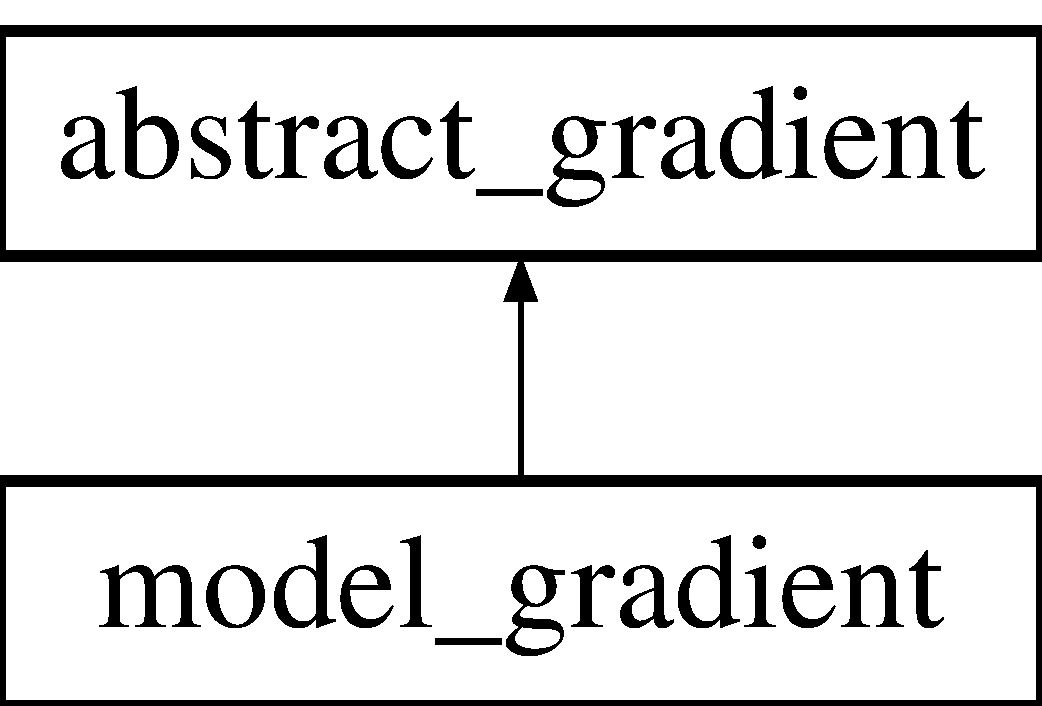
\includegraphics[height=2.000000cm]{classmodel__gradient}
\end{center}
\end{figure}
\subsection*{Public Member Functions}
\begin{DoxyCompactItemize}
\item 
\hypertarget{classmodel__gradient_a5ae08788b26aae0c8470ce93840057af}{{\bfseries model\-\_\-gradient} (sharedptr$<$ std\-::vector$<$ \hyperlink{classabstract__function}{abstract\-\_\-function} $>$ $>$ vc\-\_\-base\-\_\-functions)}\label{classmodel__gradient_a5ae08788b26aae0c8470ce93840057af}

\item 
sharedarray$<$ float $>$ \hyperlink{classmodel__gradient_a3342773b28b53352dfd08abd25b946f6}{eval} (float x, float y)
\end{DoxyCompactItemize}


\subsection{Member Function Documentation}
\hypertarget{classmodel__gradient_a3342773b28b53352dfd08abd25b946f6}{\index{model\-\_\-gradient@{model\-\_\-gradient}!eval@{eval}}
\index{eval@{eval}!model_gradient@{model\-\_\-gradient}}
\subsubsection[{eval}]{\setlength{\rightskip}{0pt plus 5cm}sharedarray$<$ float $>$ model\-\_\-gradient\-::eval (
\begin{DoxyParamCaption}
\item[{float}]{x, }
\item[{float}]{y}
\end{DoxyParamCaption}
)\hspace{0.3cm}{\ttfamily [virtual]}}}\label{classmodel__gradient_a3342773b28b53352dfd08abd25b946f6}
returns the value of the function at (x,y) 
\begin{DoxyParams}{Parameters}
{\em x} & coordinate \\
\hline
{\em y} & coordinate \\
\hline
\end{DoxyParams}
\begin{DoxyReturn}{Returns}
value of the gradient function in x and y 
\end{DoxyReturn}


Implements \hyperlink{classabstract__gradient_a4720548702baebd45572547fd913ef30}{abstract\-\_\-gradient}.



The documentation for this class was generated from the following files\-:\begin{DoxyCompactItemize}
\item 
include/model/model\-\_\-gradient.\-h\item 
src/model/model\-\_\-gradient.\-cpp\end{DoxyCompactItemize}

\hypertarget{classmonomial__function}{\section{monomial\-\_\-function Class Reference}
\label{classmonomial__function}\index{monomial\-\_\-function@{monomial\-\_\-function}}
}
Inheritance diagram for monomial\-\_\-function\-:\begin{figure}[H]
\begin{center}
\leavevmode
\includegraphics[height=2.000000cm]{classmonomial__function}
\end{center}
\end{figure}
\subsection*{Public Member Functions}
\begin{DoxyCompactItemize}
\item 
\hyperlink{classmonomial__function_a61b1594741e022f6e1f97b8b8df0b776}{monomial\-\_\-function} (int m, int n)
\item 
\hypertarget{classmonomial__function_a761359711793df68bfea7cb75401a088}{virtual \hyperlink{classmonomial__function_a761359711793df68bfea7cb75401a088}{$\sim$monomial\-\_\-function} ()}\label{classmonomial__function_a761359711793df68bfea7cb75401a088}

\begin{DoxyCompactList}\small\item\em Destruktor. \end{DoxyCompactList}\item 
float \hyperlink{classmonomial__function_ac28af6c7f8c7c48216c7bdc270598728}{eval} (float x, float y)
\item 
sharedptr$<$ \hyperlink{classabstract__gradient}{abstract\-\_\-gradient} $>$ \hyperlink{classmonomial__function_a1bb8949943f068e0597c7a8983011d12}{get\-\_\-gradient} ()
\item 
\hypertarget{classmonomial__function_af87735c8ef3441a348e10762efe84b71}{int \hyperlink{classmonomial__function_af87735c8ef3441a348e10762efe84b71}{get\-\_\-x\-\_\-exp} ()}\label{classmonomial__function_af87735c8ef3441a348e10762efe84b71}

\begin{DoxyCompactList}\small\item\em Experimental. \end{DoxyCompactList}\item 
\hypertarget{classmonomial__function_a35d7ae825a7b6d37c644a6670b8c7a23}{int \hyperlink{classmonomial__function_a35d7ae825a7b6d37c644a6670b8c7a23}{get\-\_\-y\-\_\-exp} ()}\label{classmonomial__function_a35d7ae825a7b6d37c644a6670b8c7a23}

\begin{DoxyCompactList}\small\item\em Experimental. \end{DoxyCompactList}\end{DoxyCompactItemize}


\subsection{Constructor \& Destructor Documentation}
\hypertarget{classmonomial__function_a61b1594741e022f6e1f97b8b8df0b776}{\index{monomial\-\_\-function@{monomial\-\_\-function}!monomial\-\_\-function@{monomial\-\_\-function}}
\index{monomial\-\_\-function@{monomial\-\_\-function}!monomial_function@{monomial\-\_\-function}}
\subsubsection[{monomial\-\_\-function}]{\setlength{\rightskip}{0pt plus 5cm}monomial\-\_\-function\-::monomial\-\_\-function (
\begin{DoxyParamCaption}
\item[{int}]{m, }
\item[{int}]{n}
\end{DoxyParamCaption}
)}}\label{classmonomial__function_a61b1594741e022f6e1f97b8b8df0b776}
Constructor for x$^\wedge$m $\ast$ y$^\wedge$n monomial 
\begin{DoxyParams}{Parameters}
{\em m} & power of x \\
\hline
{\em n} & power of y \\
\hline
\end{DoxyParams}


\subsection{Member Function Documentation}
\hypertarget{classmonomial__function_ac28af6c7f8c7c48216c7bdc270598728}{\index{monomial\-\_\-function@{monomial\-\_\-function}!eval@{eval}}
\index{eval@{eval}!monomial_function@{monomial\-\_\-function}}
\subsubsection[{eval}]{\setlength{\rightskip}{0pt plus 5cm}float monomial\-\_\-function\-::eval (
\begin{DoxyParamCaption}
\item[{float}]{x, }
\item[{float}]{y}
\end{DoxyParamCaption}
)\hspace{0.3cm}{\ttfamily [virtual]}}}\label{classmonomial__function_ac28af6c7f8c7c48216c7bdc270598728}
Calculate the value of this function 
\begin{DoxyParams}{Parameters}
{\em x} & coordinate \\
\hline
{\em y} & coordinate \\
\hline
\end{DoxyParams}
\begin{DoxyReturn}{Returns}
value of this function 
\end{DoxyReturn}


Implements \hyperlink{classabstract__function_ae313a63bae0ae1b88bcabd1bebc22f4f}{abstract\-\_\-function}.

\hypertarget{classmonomial__function_a1bb8949943f068e0597c7a8983011d12}{\index{monomial\-\_\-function@{monomial\-\_\-function}!get\-\_\-gradient@{get\-\_\-gradient}}
\index{get\-\_\-gradient@{get\-\_\-gradient}!monomial_function@{monomial\-\_\-function}}
\subsubsection[{get\-\_\-gradient}]{\setlength{\rightskip}{0pt plus 5cm}sharedptr$<$ {\bf abstract\-\_\-gradient} $>$ monomial\-\_\-function\-::get\-\_\-gradient (
\begin{DoxyParamCaption}
{}
\end{DoxyParamCaption}
)\hspace{0.3cm}{\ttfamily [virtual]}}}\label{classmonomial__function_a1bb8949943f068e0597c7a8983011d12}
\begin{DoxyReturn}{Returns}
sharedptr to the gradient of this function 
\end{DoxyReturn}


Implements \hyperlink{classabstract__function_a6ac83b83ed81cbd1c67ccfb9ddcf310b}{abstract\-\_\-function}.



The documentation for this class was generated from the following files\-:\begin{DoxyCompactItemize}
\item 
include/model/monomial\-\_\-function.\-h\item 
src/model/monomial\-\_\-function.\-cpp\end{DoxyCompactItemize}

\hypertarget{classmonomial__gradient}{\section{monomial\-\_\-gradient Class Reference}
\label{classmonomial__gradient}\index{monomial\-\_\-gradient@{monomial\-\_\-gradient}}
}
Inheritance diagram for monomial\-\_\-gradient\-:\begin{figure}[H]
\begin{center}
\leavevmode
\includegraphics[height=2.000000cm]{classmonomial__gradient}
\end{center}
\end{figure}
\subsection*{Public Member Functions}
\begin{DoxyCompactItemize}
\item 
\hyperlink{classmonomial__gradient_a1150cd5186763d6b59b9b01abc8e82c8}{monomial\-\_\-gradient} (int m, int n)
\item 
virtual sharedarray$<$ float $>$ \hyperlink{classmonomial__gradient_a718fe4bdf3a6edd32d655de03db8badf}{eval} (float x, float y)
\end{DoxyCompactItemize}


\subsection{Constructor \& Destructor Documentation}
\hypertarget{classmonomial__gradient_a1150cd5186763d6b59b9b01abc8e82c8}{\index{monomial\-\_\-gradient@{monomial\-\_\-gradient}!monomial\-\_\-gradient@{monomial\-\_\-gradient}}
\index{monomial\-\_\-gradient@{monomial\-\_\-gradient}!monomial_gradient@{monomial\-\_\-gradient}}
\subsubsection[{monomial\-\_\-gradient}]{\setlength{\rightskip}{0pt plus 5cm}monomial\-\_\-gradient\-::monomial\-\_\-gradient (
\begin{DoxyParamCaption}
\item[{int}]{m, }
\item[{int}]{n}
\end{DoxyParamCaption}
)}}\label{classmonomial__gradient_a1150cd5186763d6b59b9b01abc8e82c8}
Standard constructor. Takes the exponents m and n from the parent polynom. Eg. x$^\wedge$3y$^\wedge$4 calls this gradient with m = 3 \& n = 4. Conversion into the derivative comes in this constructor. 
\begin{DoxyParams}{Parameters}
{\em m} & power of x \\
\hline
{\em n} & power of y \\
\hline
\end{DoxyParams}


\subsection{Member Function Documentation}
\hypertarget{classmonomial__gradient_a718fe4bdf3a6edd32d655de03db8badf}{\index{monomial\-\_\-gradient@{monomial\-\_\-gradient}!eval@{eval}}
\index{eval@{eval}!monomial_gradient@{monomial\-\_\-gradient}}
\subsubsection[{eval}]{\setlength{\rightskip}{0pt plus 5cm}sharedarray$<$ float $>$ monomial\-\_\-gradient\-::eval (
\begin{DoxyParamCaption}
\item[{float}]{x, }
\item[{float}]{y}
\end{DoxyParamCaption}
)\hspace{0.3cm}{\ttfamily [virtual]}}}\label{classmonomial__gradient_a718fe4bdf3a6edd32d655de03db8badf}
Calculate the gradient for this function 
\begin{DoxyParams}{Parameters}
{\em x} & coordinate \\
\hline
{\em y} & coordinate \\
\hline
\end{DoxyParams}
\begin{DoxyReturn}{Returns}
2 floats, first for x-\/value 
\end{DoxyReturn}


Implements \hyperlink{classabstract__gradient_a4720548702baebd45572547fd913ef30}{abstract\-\_\-gradient}.



The documentation for this class was generated from the following files\-:\begin{DoxyCompactItemize}
\item 
include/model/monomial\-\_\-gradient.\-h\item 
src/model/monomial\-\_\-gradient.\-cpp\end{DoxyCompactItemize}

\hypertarget{classpx__floodfill__sim__ann__unwrapper}{\section{px\-\_\-floodfill\-\_\-sim\-\_\-ann\-\_\-unwrapper Class Reference}
\label{classpx__floodfill__sim__ann__unwrapper}\index{px\-\_\-floodfill\-\_\-sim\-\_\-ann\-\_\-unwrapper@{px\-\_\-floodfill\-\_\-sim\-\_\-ann\-\_\-unwrapper}}
}


{\ttfamily \#include $<$px\-\_\-floodfill\-\_\-sim\-\_\-ann\-\_\-unwrapper.\-h$>$}

Inheritance diagram for px\-\_\-floodfill\-\_\-sim\-\_\-ann\-\_\-unwrapper\-:\begin{figure}[H]
\begin{center}
\leavevmode
\includegraphics[height=2.000000cm]{classpx__floodfill__sim__ann__unwrapper}
\end{center}
\end{figure}
\subsection*{Public Member Functions}
\begin{DoxyCompactItemize}
\item 
\hypertarget{classpx__floodfill__sim__ann__unwrapper_a17701400748a2699309cc00c2056bd15}{virtual \hyperlink{classpx__floodfill__sim__ann__unwrapper_a17701400748a2699309cc00c2056bd15}{$\sim$px\-\_\-floodfill\-\_\-sim\-\_\-ann\-\_\-unwrapper} ()}\label{classpx__floodfill__sim__ann__unwrapper_a17701400748a2699309cc00c2056bd15}

\begin{DoxyCompactList}\small\item\em Destructor. \end{DoxyCompactList}\item 
\hypertarget{classpx__floodfill__sim__ann__unwrapper_a72c5c9cb7f151f50042b3d17f8b10b79}{virtual boost\-::shared\-\_\-ptr\\*
$<$ \hyperlink{classfloat__image}{float\-\_\-image} $>$ \hyperlink{classpx__floodfill__sim__ann__unwrapper_a72c5c9cb7f151f50042b3d17f8b10b79}{unwrap} (boost\-::shared\-\_\-ptr$<$ \hyperlink{classfloat__image}{float\-\_\-image} $>$ wrapped\-\_\-phase\-\_\-image)}\label{classpx__floodfill__sim__ann__unwrapper_a72c5c9cb7f151f50042b3d17f8b10b79}

\begin{DoxyCompactList}\small\item\em Unwrap the phase image. \end{DoxyCompactList}\end{DoxyCompactItemize}


\subsection{Detailed Description}
Pixelbased Floodfill Simulated Annealing Unwrapper 

The documentation for this class was generated from the following file\-:\begin{DoxyCompactItemize}
\item 
include/algorithm/px\-\_\-floodfill\-\_\-sim\-\_\-ann\-\_\-unwrapper.\-h\end{DoxyCompactItemize}

\input{classreliability__calculator__mean__difference}
\hypertarget{classreliability__calculator__random}{\section{reliability\-\_\-calculator\-\_\-random Class Reference}
\label{classreliability__calculator__random}\index{reliability\-\_\-calculator\-\_\-random@{reliability\-\_\-calculator\-\_\-random}}
}


{\ttfamily \#include $<$reliability\-\_\-calculator\-\_\-random.\-h$>$}

Inheritance diagram for reliability\-\_\-calculator\-\_\-random\-:\begin{figure}[H]
\begin{center}
\leavevmode
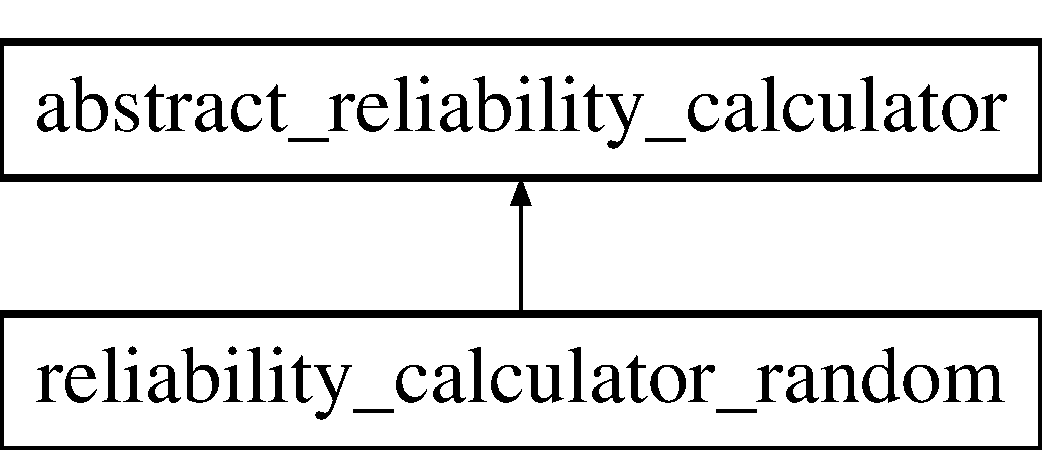
\includegraphics[height=2.000000cm]{classreliability__calculator__random}
\end{center}
\end{figure}
\subsection*{Public Member Functions}
\begin{DoxyCompactItemize}
\item 
virtual float \hyperlink{classreliability__calculator__random_a73524f3dd704cb666c794b765e4216fc}{calculate\-\_\-reliability} (boost\-::shared\-\_\-ptr$<$ \hyperlink{classtiled__image}{tiled\-\_\-image} $>$ ti, boost\-::shared\-\_\-ptr$<$ \hyperlink{classtile__junction}{tile\-\_\-junction} $>$ junc)
\item 
virtual float \hyperlink{classreliability__calculator__random_a7e49000129535b04968a5fb7a87fd5e4}{calculate\-\_\-reliability} (boost\-::shared\-\_\-ptr$<$ \hyperlink{classtiled__image}{tiled\-\_\-image} $>$ ti, boost\-::shared\-\_\-ptr$<$ \hyperlink{classtile}{tile} $>$ t)
\item 
void \hyperlink{classreliability__calculator__random_a3b5b45c3e398b70398ba139eb6046dc5}{init\-\_\-junctions} (sharedptr$<$ \hyperlink{classtiled__image}{tiled\-\_\-image} $>$ ti)
\end{DoxyCompactItemize}


\subsection{Detailed Description}
The methods of this class are just returning uniformly distributed random values between 0 and 1. This makes up a comparison to the other rel.-\/calculator regarding speed and output quality. 

\subsection{Member Function Documentation}
\hypertarget{classreliability__calculator__random_a73524f3dd704cb666c794b765e4216fc}{\index{reliability\-\_\-calculator\-\_\-random@{reliability\-\_\-calculator\-\_\-random}!calculate\-\_\-reliability@{calculate\-\_\-reliability}}
\index{calculate\-\_\-reliability@{calculate\-\_\-reliability}!reliability_calculator_random@{reliability\-\_\-calculator\-\_\-random}}
\subsubsection[{calculate\-\_\-reliability}]{\setlength{\rightskip}{0pt plus 5cm}float reliability\-\_\-calculator\-\_\-random\-::calculate\-\_\-reliability (
\begin{DoxyParamCaption}
\item[{boost\-::shared\-\_\-ptr$<$ {\bf tiled\-\_\-image} $>$}]{ti, }
\item[{boost\-::shared\-\_\-ptr$<$ {\bf tile\-\_\-junction} $>$}]{junc}
\end{DoxyParamCaption}
)\hspace{0.3cm}{\ttfamily [virtual]}}}\label{classreliability__calculator__random_a73524f3dd704cb666c794b765e4216fc}
Calculates the reliability of a given junction 
\begin{DoxyParams}{Parameters}
{\em ti} & tiled image \\
\hline
{\em junc} & junction \\
\hline
\end{DoxyParams}


Implements \hyperlink{classabstract__reliability__calculator_a0c9a7778550b643b6a273e3bf0662023}{abstract\-\_\-reliability\-\_\-calculator}.

\hypertarget{classreliability__calculator__random_a7e49000129535b04968a5fb7a87fd5e4}{\index{reliability\-\_\-calculator\-\_\-random@{reliability\-\_\-calculator\-\_\-random}!calculate\-\_\-reliability@{calculate\-\_\-reliability}}
\index{calculate\-\_\-reliability@{calculate\-\_\-reliability}!reliability_calculator_random@{reliability\-\_\-calculator\-\_\-random}}
\subsubsection[{calculate\-\_\-reliability}]{\setlength{\rightskip}{0pt plus 5cm}float reliability\-\_\-calculator\-\_\-random\-::calculate\-\_\-reliability (
\begin{DoxyParamCaption}
\item[{boost\-::shared\-\_\-ptr$<$ {\bf tiled\-\_\-image} $>$}]{ti, }
\item[{boost\-::shared\-\_\-ptr$<$ {\bf tile} $>$}]{t}
\end{DoxyParamCaption}
)\hspace{0.3cm}{\ttfamily [virtual]}}}\label{classreliability__calculator__random_a7e49000129535b04968a5fb7a87fd5e4}
Calculates the reliability of a given tile 
\begin{DoxyParams}{Parameters}
{\em ti} & tiled image \\
\hline
{\em t} & tile \\
\hline
\end{DoxyParams}


Implements \hyperlink{classabstract__reliability__calculator_a496b1743c17660ae4617eebdd312bb9d}{abstract\-\_\-reliability\-\_\-calculator}.

\hypertarget{classreliability__calculator__random_a3b5b45c3e398b70398ba139eb6046dc5}{\index{reliability\-\_\-calculator\-\_\-random@{reliability\-\_\-calculator\-\_\-random}!init\-\_\-junctions@{init\-\_\-junctions}}
\index{init\-\_\-junctions@{init\-\_\-junctions}!reliability_calculator_random@{reliability\-\_\-calculator\-\_\-random}}
\subsubsection[{init\-\_\-junctions}]{\setlength{\rightskip}{0pt plus 5cm}void reliability\-\_\-calculator\-\_\-random\-::init\-\_\-junctions (
\begin{DoxyParamCaption}
\item[{sharedptr$<$ {\bf tiled\-\_\-image} $>$}]{ti}
\end{DoxyParamCaption}
)\hspace{0.3cm}{\ttfamily [virtual]}}}\label{classreliability__calculator__random_a3b5b45c3e398b70398ba139eb6046dc5}
E\-M\-P\-T\-Y 
\begin{DoxyParams}{Parameters}
{\em ti} & tiled image \\
\hline
\end{DoxyParams}


Implements \hyperlink{classabstract__reliability__calculator_a4457d3eece3c873e2cc2455a6dfdbb88}{abstract\-\_\-reliability\-\_\-calculator}.



The documentation for this class was generated from the following files\-:\begin{DoxyCompactItemize}
\item 
include/algorithm/reliability\-\_\-calculator\-\_\-random.\-h\item 
src/algorithm/reliability\-\_\-calculator\-\_\-random.\-cpp\end{DoxyCompactItemize}

\hypertarget{classreliability__calculator__variance}{\section{reliability\-\_\-calculator\-\_\-variance Class Reference}
\label{classreliability__calculator__variance}\index{reliability\-\_\-calculator\-\_\-variance@{reliability\-\_\-calculator\-\_\-variance}}
}
Inheritance diagram for reliability\-\_\-calculator\-\_\-variance\-:\begin{figure}[H]
\begin{center}
\leavevmode
\includegraphics[height=2.000000cm]{classreliability__calculator__variance}
\end{center}
\end{figure}
\subsection*{Public Member Functions}
\begin{DoxyCompactItemize}
\item 
\hypertarget{classreliability__calculator__variance_aa97b8fa061b578f6be66a89afba64657}{\hyperlink{classreliability__calculator__variance_aa97b8fa061b578f6be66a89afba64657}{reliability\-\_\-calculator\-\_\-variance} ()}\label{classreliability__calculator__variance_aa97b8fa061b578f6be66a89afba64657}

\begin{DoxyCompactList}\small\item\em Std Constructor. \end{DoxyCompactList}\item 
virtual float \hyperlink{classreliability__calculator__variance_ac6380a3bedfdc5648f501cd0a5c92369}{calculate\-\_\-reliability} (boost\-::shared\-\_\-ptr$<$ \hyperlink{classtiled__image}{tiled\-\_\-image} $>$ ti, boost\-::shared\-\_\-ptr$<$ \hyperlink{classtile__junction}{tile\-\_\-junction} $>$ t)
\item 
virtual float \hyperlink{classreliability__calculator__variance_a0250bc0b9f2d62ec48b66449d6f94b56}{calculate\-\_\-reliability} (boost\-::shared\-\_\-ptr$<$ \hyperlink{classtiled__image}{tiled\-\_\-image} $>$ ti, boost\-::shared\-\_\-ptr$<$ \hyperlink{classtile}{tile} $>$ t)
\item 
void \hyperlink{classreliability__calculator__variance_ad371792568036db7a8dac6fabbb78d05}{init\-\_\-junctions} (sharedptr$<$ \hyperlink{classtiled__image}{tiled\-\_\-image} $>$ ti)
\end{DoxyCompactItemize}


\subsection{Member Function Documentation}
\hypertarget{classreliability__calculator__variance_ac6380a3bedfdc5648f501cd0a5c92369}{\index{reliability\-\_\-calculator\-\_\-variance@{reliability\-\_\-calculator\-\_\-variance}!calculate\-\_\-reliability@{calculate\-\_\-reliability}}
\index{calculate\-\_\-reliability@{calculate\-\_\-reliability}!reliability_calculator_variance@{reliability\-\_\-calculator\-\_\-variance}}
\subsubsection[{calculate\-\_\-reliability}]{\setlength{\rightskip}{0pt plus 5cm}float reliability\-\_\-calculator\-\_\-variance\-::calculate\-\_\-reliability (
\begin{DoxyParamCaption}
\item[{boost\-::shared\-\_\-ptr$<$ {\bf tiled\-\_\-image} $>$}]{ti, }
\item[{boost\-::shared\-\_\-ptr$<$ {\bf tile\-\_\-junction} $>$}]{t}
\end{DoxyParamCaption}
)\hspace{0.3cm}{\ttfamily [virtual]}}}\label{classreliability__calculator__variance_ac6380a3bedfdc5648f501cd0a5c92369}
Calculates the reliability of a given junction 
\begin{DoxyParams}{Parameters}
{\em ti} & tiled image \\
\hline
{\em t} & junction \\
\hline
\end{DoxyParams}
\begin{DoxyReturn}{Returns}
float between 0 and F\-L\-T\-\_\-\-M\-A\-X 
\end{DoxyReturn}


Implements \hyperlink{classabstract__reliability__calculator_a0c9a7778550b643b6a273e3bf0662023}{abstract\-\_\-reliability\-\_\-calculator}.

\hypertarget{classreliability__calculator__variance_a0250bc0b9f2d62ec48b66449d6f94b56}{\index{reliability\-\_\-calculator\-\_\-variance@{reliability\-\_\-calculator\-\_\-variance}!calculate\-\_\-reliability@{calculate\-\_\-reliability}}
\index{calculate\-\_\-reliability@{calculate\-\_\-reliability}!reliability_calculator_variance@{reliability\-\_\-calculator\-\_\-variance}}
\subsubsection[{calculate\-\_\-reliability}]{\setlength{\rightskip}{0pt plus 5cm}float reliability\-\_\-calculator\-\_\-variance\-::calculate\-\_\-reliability (
\begin{DoxyParamCaption}
\item[{boost\-::shared\-\_\-ptr$<$ {\bf tiled\-\_\-image} $>$}]{ti, }
\item[{boost\-::shared\-\_\-ptr$<$ {\bf tile} $>$}]{t}
\end{DoxyParamCaption}
)\hspace{0.3cm}{\ttfamily [virtual]}}}\label{classreliability__calculator__variance_a0250bc0b9f2d62ec48b66449d6f94b56}
Calculates the reliability of a given tile 
\begin{DoxyParams}{Parameters}
{\em ti} & tiled image \\
\hline
{\em t} & junction \\
\hline
\end{DoxyParams}
\begin{DoxyReturn}{Returns}
float between 0 and F\-L\-T\-\_\-\-M\-A\-X (or inf) 
\end{DoxyReturn}


Implements \hyperlink{classabstract__reliability__calculator_a496b1743c17660ae4617eebdd312bb9d}{abstract\-\_\-reliability\-\_\-calculator}.

\hypertarget{classreliability__calculator__variance_ad371792568036db7a8dac6fabbb78d05}{\index{reliability\-\_\-calculator\-\_\-variance@{reliability\-\_\-calculator\-\_\-variance}!init\-\_\-junctions@{init\-\_\-junctions}}
\index{init\-\_\-junctions@{init\-\_\-junctions}!reliability_calculator_variance@{reliability\-\_\-calculator\-\_\-variance}}
\subsubsection[{init\-\_\-junctions}]{\setlength{\rightskip}{0pt plus 5cm}void reliability\-\_\-calculator\-\_\-variance\-::init\-\_\-junctions (
\begin{DoxyParamCaption}
\item[{sharedptr$<$ {\bf tiled\-\_\-image} $>$}]{ti}
\end{DoxyParamCaption}
)\hspace{0.3cm}{\ttfamily [virtual]}}}\label{classreliability__calculator__variance_ad371792568036db7a8dac6fabbb78d05}
Calculate the variance of each junction once, therefore making it possible to just access them via get\-\_\-variance. 
\begin{DoxyParams}{Parameters}
{\em ti} & tiled image \\
\hline
\end{DoxyParams}


Implements \hyperlink{classabstract__reliability__calculator_a4457d3eece3c873e2cc2455a6dfdbb88}{abstract\-\_\-reliability\-\_\-calculator}.



The documentation for this class was generated from the following files\-:\begin{DoxyCompactItemize}
\item 
include/algorithm/reliability\-\_\-calculator\-\_\-variance.\-h\item 
src/algorithm/reliability\-\_\-calculator\-\_\-variance.\-cpp\end{DoxyCompactItemize}

\hypertarget{classreliability__calculator__variance__second}{\section{reliability\-\_\-calculator\-\_\-variance\-\_\-second Class Reference}
\label{classreliability__calculator__variance__second}\index{reliability\-\_\-calculator\-\_\-variance\-\_\-second@{reliability\-\_\-calculator\-\_\-variance\-\_\-second}}
}
Inheritance diagram for reliability\-\_\-calculator\-\_\-variance\-\_\-second\-:\begin{figure}[H]
\begin{center}
\leavevmode
\includegraphics[height=2.000000cm]{classreliability__calculator__variance__second}
\end{center}
\end{figure}
\subsection*{Public Member Functions}
\begin{DoxyCompactItemize}
\item 
virtual float \hyperlink{classreliability__calculator__variance__second_a1150171c57a7b9420e5f5211e71c265a}{calculate\-\_\-reliability} (boost\-::shared\-\_\-ptr$<$ \hyperlink{classtiled__image}{tiled\-\_\-image} $>$ ti, boost\-::shared\-\_\-ptr$<$ \hyperlink{classtile__junction}{tile\-\_\-junction} $>$ t)
\item 
virtual float \hyperlink{classreliability__calculator__variance__second_a0cab62b334c6f20aa821496f7364bd98}{calculate\-\_\-reliability} (boost\-::shared\-\_\-ptr$<$ \hyperlink{classtiled__image}{tiled\-\_\-image} $>$ ti, boost\-::shared\-\_\-ptr$<$ \hyperlink{classtile}{tile} $>$ t)
\item 
void \hyperlink{classreliability__calculator__variance__second_a5c7dcb23c303a0ec762504ea9a775b2b}{init\-\_\-junctions} (sharedptr$<$ \hyperlink{classtiled__image}{tiled\-\_\-image} $>$ ti)
\end{DoxyCompactItemize}


\subsection{Member Function Documentation}
\hypertarget{classreliability__calculator__variance__second_a1150171c57a7b9420e5f5211e71c265a}{\index{reliability\-\_\-calculator\-\_\-variance\-\_\-second@{reliability\-\_\-calculator\-\_\-variance\-\_\-second}!calculate\-\_\-reliability@{calculate\-\_\-reliability}}
\index{calculate\-\_\-reliability@{calculate\-\_\-reliability}!reliability_calculator_variance_second@{reliability\-\_\-calculator\-\_\-variance\-\_\-second}}
\subsubsection[{calculate\-\_\-reliability}]{\setlength{\rightskip}{0pt plus 5cm}float reliability\-\_\-calculator\-\_\-variance\-\_\-second\-::calculate\-\_\-reliability (
\begin{DoxyParamCaption}
\item[{boost\-::shared\-\_\-ptr$<$ {\bf tiled\-\_\-image} $>$}]{ti, }
\item[{boost\-::shared\-\_\-ptr$<$ {\bf tile\-\_\-junction} $>$}]{t}
\end{DoxyParamCaption}
)\hspace{0.3cm}{\ttfamily [virtual]}}}\label{classreliability__calculator__variance__second_a1150171c57a7b9420e5f5211e71c265a}
Calculates the reliability of a given junction 
\begin{DoxyParams}{Parameters}
{\em ti} & tiled image \\
\hline
{\em t} & junction \\
\hline
\end{DoxyParams}
\begin{DoxyReturn}{Returns}
float between 0 and F\-L\-T\-\_\-\-M\-A\-X/2 
\end{DoxyReturn}


Implements \hyperlink{classabstract__reliability__calculator_a0c9a7778550b643b6a273e3bf0662023}{abstract\-\_\-reliability\-\_\-calculator}.

\hypertarget{classreliability__calculator__variance__second_a0cab62b334c6f20aa821496f7364bd98}{\index{reliability\-\_\-calculator\-\_\-variance\-\_\-second@{reliability\-\_\-calculator\-\_\-variance\-\_\-second}!calculate\-\_\-reliability@{calculate\-\_\-reliability}}
\index{calculate\-\_\-reliability@{calculate\-\_\-reliability}!reliability_calculator_variance_second@{reliability\-\_\-calculator\-\_\-variance\-\_\-second}}
\subsubsection[{calculate\-\_\-reliability}]{\setlength{\rightskip}{0pt plus 5cm}float reliability\-\_\-calculator\-\_\-variance\-\_\-second\-::calculate\-\_\-reliability (
\begin{DoxyParamCaption}
\item[{boost\-::shared\-\_\-ptr$<$ {\bf tiled\-\_\-image} $>$}]{ti, }
\item[{boost\-::shared\-\_\-ptr$<$ {\bf tile} $>$}]{t}
\end{DoxyParamCaption}
)\hspace{0.3cm}{\ttfamily [virtual]}}}\label{classreliability__calculator__variance__second_a0cab62b334c6f20aa821496f7364bd98}
Calculates the reliability of a given tile 
\begin{DoxyParams}{Parameters}
{\em ti} & tiled image \\
\hline
{\em t} & junction \\
\hline
\end{DoxyParams}
\begin{DoxyReturn}{Returns}
float between 0 and F\-L\-T\-\_\-\-M\-A\-X 
\end{DoxyReturn}


Implements \hyperlink{classabstract__reliability__calculator_a496b1743c17660ae4617eebdd312bb9d}{abstract\-\_\-reliability\-\_\-calculator}.

\hypertarget{classreliability__calculator__variance__second_a5c7dcb23c303a0ec762504ea9a775b2b}{\index{reliability\-\_\-calculator\-\_\-variance\-\_\-second@{reliability\-\_\-calculator\-\_\-variance\-\_\-second}!init\-\_\-junctions@{init\-\_\-junctions}}
\index{init\-\_\-junctions@{init\-\_\-junctions}!reliability_calculator_variance_second@{reliability\-\_\-calculator\-\_\-variance\-\_\-second}}
\subsubsection[{init\-\_\-junctions}]{\setlength{\rightskip}{0pt plus 5cm}void reliability\-\_\-calculator\-\_\-variance\-\_\-second\-::init\-\_\-junctions (
\begin{DoxyParamCaption}
\item[{sharedptr$<$ {\bf tiled\-\_\-image} $>$}]{ti}
\end{DoxyParamCaption}
)\hspace{0.3cm}{\ttfamily [virtual]}}}\label{classreliability__calculator__variance__second_a5c7dcb23c303a0ec762504ea9a775b2b}
Calculate the variance of each junction once, therefor making it possible to just access them via get\-\_\-variance. 
\begin{DoxyParams}{Parameters}
{\em ti} & tiled image \\
\hline
\end{DoxyParams}


Implements \hyperlink{classabstract__reliability__calculator_a4457d3eece3c873e2cc2455a6dfdbb88}{abstract\-\_\-reliability\-\_\-calculator}.



The documentation for this class was generated from the following files\-:\begin{DoxyCompactItemize}
\item 
include/algorithm/reliability\-\_\-calculator\-\_\-variance\-\_\-second.\-h\item 
src/algorithm/reliability\-\_\-calculator\-\_\-variance\-\_\-second.\-cpp\end{DoxyCompactItemize}

\hypertarget{classrow__major__float__image}{\section{row\-\_\-major\-\_\-float\-\_\-image Class Reference}
\label{classrow__major__float__image}\index{row\-\_\-major\-\_\-float\-\_\-image@{row\-\_\-major\-\_\-float\-\_\-image}}
}
Inheritance diagram for row\-\_\-major\-\_\-float\-\_\-image\-:\begin{figure}[H]
\begin{center}
\leavevmode
\includegraphics[height=2.000000cm]{classrow__major__float__image}
\end{center}
\end{figure}
\subsection*{Public Member Functions}
\begin{DoxyCompactItemize}
\item 
\hypertarget{classrow__major__float__image_a2aa84173f1aa9a37795e6b8d36642983}{{\bfseries row\-\_\-major\-\_\-float\-\_\-image} (float $\ast$data, long width, long height)}\label{classrow__major__float__image_a2aa84173f1aa9a37795e6b8d36642983}

\item 
\hyperlink{classrow__major__float__image_a918e2036b3d18fd6344f2edecd309891}{row\-\_\-major\-\_\-float\-\_\-image} (long width, long height)
\item 
virtual float \& \hyperlink{classrow__major__float__image_a04b9b253a3771e0963c839a9a85ccd99}{operator()} (long w, long h)
\item 
\hypertarget{classrow__major__float__image_af38e45798ef162384d75ad5c60cb40d0}{virtual float {\bfseries operator()} (long w, long h) const }\label{classrow__major__float__image_af38e45798ef162384d75ad5c60cb40d0}

\end{DoxyCompactItemize}
\subsection*{Additional Inherited Members}


\subsection{Constructor \& Destructor Documentation}
\hypertarget{classrow__major__float__image_a918e2036b3d18fd6344f2edecd309891}{\index{row\-\_\-major\-\_\-float\-\_\-image@{row\-\_\-major\-\_\-float\-\_\-image}!row\-\_\-major\-\_\-float\-\_\-image@{row\-\_\-major\-\_\-float\-\_\-image}}
\index{row\-\_\-major\-\_\-float\-\_\-image@{row\-\_\-major\-\_\-float\-\_\-image}!row_major_float_image@{row\-\_\-major\-\_\-float\-\_\-image}}
\subsubsection[{row\-\_\-major\-\_\-float\-\_\-image}]{\setlength{\rightskip}{0pt plus 5cm}row\-\_\-major\-\_\-float\-\_\-image\-::row\-\_\-major\-\_\-float\-\_\-image (
\begin{DoxyParamCaption}
\item[{long}]{width, }
\item[{long}]{height}
\end{DoxyParamCaption}
)\hspace{0.3cm}{\ttfamily [inline]}}}\label{classrow__major__float__image_a918e2036b3d18fd6344f2edecd309891}
Generate image that reserves memory 
\begin{DoxyParams}{Parameters}
{\em width} & \\
\hline
{\em height} & \\
\hline
\end{DoxyParams}


\subsection{Member Function Documentation}
\hypertarget{classrow__major__float__image_a04b9b253a3771e0963c839a9a85ccd99}{\index{row\-\_\-major\-\_\-float\-\_\-image@{row\-\_\-major\-\_\-float\-\_\-image}!operator()@{operator()}}
\index{operator()@{operator()}!row_major_float_image@{row\-\_\-major\-\_\-float\-\_\-image}}
\subsubsection[{operator()}]{\setlength{\rightskip}{0pt plus 5cm}float \& row\-\_\-major\-\_\-float\-\_\-image\-::operator() (
\begin{DoxyParamCaption}
\item[{long}]{w, }
\item[{long}]{h}
\end{DoxyParamCaption}
)\hspace{0.3cm}{\ttfamily [virtual]}}}\label{classrow__major__float__image_a04b9b253a3771e0963c839a9a85ccd99}
Return element at position width = w, height = h, starting with (0,0) in upper left corner of the image. Implemented in child classes, see e.\-g. \hyperlink{classrow__major__float__image}{row\-\_\-major\-\_\-float\-\_\-image}. 

Implements \hyperlink{classfloat__image_a62e1446efb51fadcfeebf50568f9d1e9}{float\-\_\-image}.



The documentation for this class was generated from the following files\-:\begin{DoxyCompactItemize}
\item 
include/row\-\_\-major\-\_\-float\-\_\-image.\-h\item 
src/row\-\_\-major\-\_\-float\-\_\-image.\-cpp\end{DoxyCompactItemize}

\hypertarget{classsecond__order__gradient}{\section{second\-\_\-order\-\_\-gradient Class Reference}
\label{classsecond__order__gradient}\index{second\-\_\-order\-\_\-gradient@{second\-\_\-order\-\_\-gradient}}
}


{\ttfamily \#include $<$second\-\_\-order\-\_\-gradient.\-h$>$}

Inheritance diagram for second\-\_\-order\-\_\-gradient\-:\begin{figure}[H]
\begin{center}
\leavevmode
\includegraphics[height=2.000000cm]{classsecond__order__gradient}
\end{center}
\end{figure}
\subsection*{Public Member Functions}
\begin{DoxyCompactItemize}
\item 
\hypertarget{classsecond__order__gradient_ab188e5caf3d7739c254e181197766adb}{\hyperlink{classsecond__order__gradient_ab188e5caf3d7739c254e181197766adb}{second\-\_\-order\-\_\-gradient} ()}\label{classsecond__order__gradient_ab188e5caf3d7739c254e181197766adb}

\begin{DoxyCompactList}\small\item\em Std Constructor. This class always uses a cartesian\-\_\-unit\-\_\-coordinate system as the underlying coordinate system. \end{DoxyCompactList}\item 
\hypertarget{classsecond__order__gradient_a2ba4cf69f1e941099a618d1b6a9c5f2a}{\hyperlink{classsecond__order__gradient_a2ba4cf69f1e941099a618d1b6a9c5f2a}{second\-\_\-order\-\_\-gradient} (sharedptr$<$ \hyperlink{classabstract__coordinate__system}{abstract\-\_\-coordinate\-\_\-system} $>$ coord\-\_\-sys)}\label{classsecond__order__gradient_a2ba4cf69f1e941099a618d1b6a9c5f2a}

\begin{DoxyCompactList}\small\item\em Constructor. \end{DoxyCompactList}\item 
\hypertarget{classsecond__order__gradient_a4adcb194a263b8eb0cb9162dd0f272d8}{virtual \hyperlink{classsecond__order__gradient_a4adcb194a263b8eb0cb9162dd0f272d8}{$\sim$second\-\_\-order\-\_\-gradient} ()}\label{classsecond__order__gradient_a4adcb194a263b8eb0cb9162dd0f272d8}

\begin{DoxyCompactList}\small\item\em Destructor. \end{DoxyCompactList}\item 
sharedptr$<$ std\-::vector$<$ float $>$ $>$ \hyperlink{classsecond__order__gradient_a611bd811d9a47b0a53b7a827344189ff}{get\-\_\-gradient\-\_\-floats} (sharedptr$<$ \hyperlink{classtile}{tile} $>$ t)
\item 
sharedptr$<$ Eigen\-::\-Vector\-Xf $>$ \hyperlink{classsecond__order__gradient_a920ecf0cbc89fa73782a318186cc3a6b}{get\-\_\-gradient\-\_\-eigen\-\_\-vector} (sharedptr$<$ \hyperlink{classtile}{tile} $>$ t)
\end{DoxyCompactItemize}


\subsection{Detailed Description}
This class calculates the numerical derivative of a tile using a cartesian\-\_\-unit\-\_\-coordinate system as the underlying coordinate system of each tile. 

\subsection{Member Function Documentation}
\hypertarget{classsecond__order__gradient_a920ecf0cbc89fa73782a318186cc3a6b}{\index{second\-\_\-order\-\_\-gradient@{second\-\_\-order\-\_\-gradient}!get\-\_\-gradient\-\_\-eigen\-\_\-vector@{get\-\_\-gradient\-\_\-eigen\-\_\-vector}}
\index{get\-\_\-gradient\-\_\-eigen\-\_\-vector@{get\-\_\-gradient\-\_\-eigen\-\_\-vector}!second_order_gradient@{second\-\_\-order\-\_\-gradient}}
\subsubsection[{get\-\_\-gradient\-\_\-eigen\-\_\-vector}]{\setlength{\rightskip}{0pt plus 5cm}sharedptr$<$ Eigen\-::\-Vector\-Xf $>$ second\-\_\-order\-\_\-gradient\-::get\-\_\-gradient\-\_\-eigen\-\_\-vector (
\begin{DoxyParamCaption}
\item[{sharedptr$<$ {\bf tile} $>$}]{t}
\end{DoxyParamCaption}
)\hspace{0.3cm}{\ttfamily [virtual]}}}\label{classsecond__order__gradient_a920ecf0cbc89fa73782a318186cc3a6b}
Get the gradient of a given tile as a Eigen\-::\-Vector of floats 
\begin{DoxyParams}{Parameters}
{\em t} & tile \\
\hline
\end{DoxyParams}
\begin{DoxyReturn}{Returns}
Eigen\-::vector of floats, first holds the x-\/gradient-\/values in order of tile has in its vector. Second holds y... 
\end{DoxyReturn}


Implements \hyperlink{classabstract__gradient__calculator_ae101a124df59f5dbcc4d21acffe43ae1}{abstract\-\_\-gradient\-\_\-calculator}.

\hypertarget{classsecond__order__gradient_a611bd811d9a47b0a53b7a827344189ff}{\index{second\-\_\-order\-\_\-gradient@{second\-\_\-order\-\_\-gradient}!get\-\_\-gradient\-\_\-floats@{get\-\_\-gradient\-\_\-floats}}
\index{get\-\_\-gradient\-\_\-floats@{get\-\_\-gradient\-\_\-floats}!second_order_gradient@{second\-\_\-order\-\_\-gradient}}
\subsubsection[{get\-\_\-gradient\-\_\-floats}]{\setlength{\rightskip}{0pt plus 5cm}sharedptr$<$ std\-::vector$<$ float $>$ $>$ second\-\_\-order\-\_\-gradient\-::get\-\_\-gradient\-\_\-floats (
\begin{DoxyParamCaption}
\item[{sharedptr$<$ {\bf tile} $>$}]{t}
\end{DoxyParamCaption}
)\hspace{0.3cm}{\ttfamily [virtual]}}}\label{classsecond__order__gradient_a611bd811d9a47b0a53b7a827344189ff}
Get the gradient of a given tile as raw float data 
\begin{DoxyParams}{Parameters}
{\em t} & tile \\
\hline
\end{DoxyParams}
\begin{DoxyReturn}{Returns}
vector of floats, first holds the x-\/gradient-\/values in order of tile has in its vector. Second holds y... 
\end{DoxyReturn}


Implements \hyperlink{classabstract__gradient__calculator_afbc6ee285d21d21b2241cfe643f8adce}{abstract\-\_\-gradient\-\_\-calculator}.



The documentation for this class was generated from the following files\-:\begin{DoxyCompactItemize}
\item 
include/algorithm/second\-\_\-order\-\_\-gradient.\-h\item 
src/algorithm/second\-\_\-order\-\_\-gradient.\-cpp\end{DoxyCompactItemize}

\hypertarget{classsimple1d__tile__merger}{\section{simple1d\-\_\-tile\-\_\-merger Class Reference}
\label{classsimple1d__tile__merger}\index{simple1d\-\_\-tile\-\_\-merger@{simple1d\-\_\-tile\-\_\-merger}}
}
Inheritance diagram for simple1d\-\_\-tile\-\_\-merger\-:\begin{figure}[H]
\begin{center}
\leavevmode
\includegraphics[height=2.000000cm]{classsimple1d__tile__merger}
\end{center}
\end{figure}
\subsection*{Public Member Functions}
\begin{DoxyCompactItemize}
\item 
\hyperlink{classsimple1d__tile__merger_a81b44df8dc122d9f7a5ab84f34aa5bed}{simple1d\-\_\-tile\-\_\-merger} ()
\item 
\hyperlink{classsimple1d__tile__merger_aaa0bc848ba9949cdf7d3b7a3021f00a9}{simple1d\-\_\-tile\-\_\-merger} (bool left2right, bool top2bottom, bool start\-\_\-horizontal)
\item 
virtual void \hyperlink{classsimple1d__tile__merger_ad73f710dd3ea0116859dcf2e5f6c5a14}{merge\-\_\-tiles} (boost\-::shared\-\_\-ptr$<$ \hyperlink{classtiled__image}{tiled\-\_\-image} $>$ ti)
\item 
virtual std\-::string \hyperlink{classsimple1d__tile__merger_ac0810b20cdeb08613cb2a214267cf26a}{get\-\_\-name} ()
\item 
virtual void \hyperlink{classsimple1d__tile__merger_a4f18628ddf20f24efc13e705b469268c}{usage\-\_\-help} ()
\end{DoxyCompactItemize}


\subsection{Constructor \& Destructor Documentation}
\hypertarget{classsimple1d__tile__merger_a81b44df8dc122d9f7a5ab84f34aa5bed}{\index{simple1d\-\_\-tile\-\_\-merger@{simple1d\-\_\-tile\-\_\-merger}!simple1d\-\_\-tile\-\_\-merger@{simple1d\-\_\-tile\-\_\-merger}}
\index{simple1d\-\_\-tile\-\_\-merger@{simple1d\-\_\-tile\-\_\-merger}!simple1d_tile_merger@{simple1d\-\_\-tile\-\_\-merger}}
\subsubsection[{simple1d\-\_\-tile\-\_\-merger}]{\setlength{\rightskip}{0pt plus 5cm}simple1d\-\_\-tile\-\_\-merger\-::simple1d\-\_\-tile\-\_\-merger (
\begin{DoxyParamCaption}
{}
\end{DoxyParamCaption}
)}}\label{classsimple1d__tile__merger_a81b44df8dc122d9f7a5ab84f34aa5bed}
Linear unwrapper based on 1d unwrapping of blocks. \hypertarget{classsimple1d__tile__merger_aaa0bc848ba9949cdf7d3b7a3021f00a9}{\index{simple1d\-\_\-tile\-\_\-merger@{simple1d\-\_\-tile\-\_\-merger}!simple1d\-\_\-tile\-\_\-merger@{simple1d\-\_\-tile\-\_\-merger}}
\index{simple1d\-\_\-tile\-\_\-merger@{simple1d\-\_\-tile\-\_\-merger}!simple1d_tile_merger@{simple1d\-\_\-tile\-\_\-merger}}
\subsubsection[{simple1d\-\_\-tile\-\_\-merger}]{\setlength{\rightskip}{0pt plus 5cm}simple1d\-\_\-tile\-\_\-merger\-::simple1d\-\_\-tile\-\_\-merger (
\begin{DoxyParamCaption}
\item[{bool}]{left2right, }
\item[{bool}]{top2bottom, }
\item[{bool}]{start\-\_\-horizontal}
\end{DoxyParamCaption}
)}}\label{classsimple1d__tile__merger_aaa0bc848ba9949cdf7d3b7a3021f00a9}
Linear unwrapper based on 1d unwrapping of blocks.\-The booleans are useful if the image has discontinuties on the edges. 
\begin{DoxyParams}{Parameters}
{\em left2right} & Specify the horizontal direction of merging\-: true\-: Start left and head right. false\-: right to left. \\
\hline
{\em top2bottom} & Specify the vertical direction of merging\-: true\-: Start from the top to the bottom edge. false\-: bottom to top. \\
\hline
{\em start\-\_\-horizontal} & Specify order of merging\-: true\-: First merge horizontal, then vertical. false\-: First vertical, then horizontal \\
\hline
\end{DoxyParams}


\subsection{Member Function Documentation}
\hypertarget{classsimple1d__tile__merger_ac0810b20cdeb08613cb2a214267cf26a}{\index{simple1d\-\_\-tile\-\_\-merger@{simple1d\-\_\-tile\-\_\-merger}!get\-\_\-name@{get\-\_\-name}}
\index{get\-\_\-name@{get\-\_\-name}!simple1d_tile_merger@{simple1d\-\_\-tile\-\_\-merger}}
\subsubsection[{get\-\_\-name}]{\setlength{\rightskip}{0pt plus 5cm}std\-::string simple1d\-\_\-tile\-\_\-merger\-::get\-\_\-name (
\begin{DoxyParamCaption}
{}
\end{DoxyParamCaption}
)\hspace{0.3cm}{\ttfamily [virtual]}}}\label{classsimple1d__tile__merger_ac0810b20cdeb08613cb2a214267cf26a}
Return a name (with options) to set in the output file name 

Implements \hyperlink{classabstract__tile__merger_a12ec9d118912b3c571d61ff9649042c6}{abstract\-\_\-tile\-\_\-merger}.

\hypertarget{classsimple1d__tile__merger_ad73f710dd3ea0116859dcf2e5f6c5a14}{\index{simple1d\-\_\-tile\-\_\-merger@{simple1d\-\_\-tile\-\_\-merger}!merge\-\_\-tiles@{merge\-\_\-tiles}}
\index{merge\-\_\-tiles@{merge\-\_\-tiles}!simple1d_tile_merger@{simple1d\-\_\-tile\-\_\-merger}}
\subsubsection[{merge\-\_\-tiles}]{\setlength{\rightskip}{0pt plus 5cm}void simple1d\-\_\-tile\-\_\-merger\-::merge\-\_\-tiles (
\begin{DoxyParamCaption}
\item[{boost\-::shared\-\_\-ptr$<$ {\bf tiled\-\_\-image} $>$}]{ti}
\end{DoxyParamCaption}
)\hspace{0.3cm}{\ttfamily [virtual]}}}\label{classsimple1d__tile__merger_ad73f710dd3ea0116859dcf2e5f6c5a14}
Merge tiles of a tiled image. The tiles have to be unwrapped inside themselves. This method unwraps the tiles with respect to each other. The phase discontinuity between each tile must be integer multiples of 2\-P\-I. 
\begin{DoxyParams}{Parameters}
{\em ti} & boost shared\-\_\-ptr to smart tiled image \\
\hline
\end{DoxyParams}


Implements \hyperlink{classabstract__tile__merger_a52ab494f77e495ab1a59b49e49c98db4}{abstract\-\_\-tile\-\_\-merger}.

\hypertarget{classsimple1d__tile__merger_a4f18628ddf20f24efc13e705b469268c}{\index{simple1d\-\_\-tile\-\_\-merger@{simple1d\-\_\-tile\-\_\-merger}!usage\-\_\-help@{usage\-\_\-help}}
\index{usage\-\_\-help@{usage\-\_\-help}!simple1d_tile_merger@{simple1d\-\_\-tile\-\_\-merger}}
\subsubsection[{usage\-\_\-help}]{\setlength{\rightskip}{0pt plus 5cm}void simple1d\-\_\-tile\-\_\-merger\-::usage\-\_\-help (
\begin{DoxyParamCaption}
{}
\end{DoxyParamCaption}
)\hspace{0.3cm}{\ttfamily [virtual]}}}\label{classsimple1d__tile__merger_a4f18628ddf20f24efc13e705b469268c}
Display a help on how to use this merger, in particular usage of merger-\/settings 

Implements \hyperlink{classabstract__tile__merger_a7922b65624d12ef2d6c115218d2378b4}{abstract\-\_\-tile\-\_\-merger}.



The documentation for this class was generated from the following files\-:\begin{DoxyCompactItemize}
\item 
include/algorithm/simple1d\-\_\-tile\-\_\-merger.\-h\item 
src/algorithm/simple1d\-\_\-tile\-\_\-merger.\-cpp\end{DoxyCompactItemize}

\hypertarget{classsimulated__annealing__floodfill__merger}{\section{simulated\-\_\-annealing\-\_\-floodfill\-\_\-merger Class Reference}
\label{classsimulated__annealing__floodfill__merger}\index{simulated\-\_\-annealing\-\_\-floodfill\-\_\-merger@{simulated\-\_\-annealing\-\_\-floodfill\-\_\-merger}}
}
Inheritance diagram for simulated\-\_\-annealing\-\_\-floodfill\-\_\-merger\-:\begin{figure}[H]
\begin{center}
\leavevmode
\includegraphics[height=2.000000cm]{classsimulated__annealing__floodfill__merger}
\end{center}
\end{figure}
\subsection*{Public Member Functions}
\begin{DoxyCompactItemize}
\item 
\hyperlink{classsimulated__annealing__floodfill__merger_a55d824fc05eb37d45888ecc2e2439250}{simulated\-\_\-annealing\-\_\-floodfill\-\_\-merger} (std\-::vector$<$ std\-::string $>$ msettings)
\item 
\hyperlink{classsimulated__annealing__floodfill__merger_a6ed9571eaf0051f48c9502d00f334802}{simulated\-\_\-annealing\-\_\-floodfill\-\_\-merger} (int check\-\_\-steps, float convergence\-\_\-criterion, std\-::string merge\-\_\-prior, float name\-\_\-energy\-\_\-after\-\_\-merging, float name\-\_\-energy\-\_\-prior\-\_\-merging, bool name\-\_\-extended, int name\-\_\-steps\-\_\-to\-\_\-convergence, long seed, int series\-\_\-start, int series\-\_\-steps, int series\-\_\-stop, float temperature, float good\-\_\-mean, float good\-\_\-variance)
\item 
virtual void \hyperlink{classsimulated__annealing__floodfill__merger_a4d15f1b8e98b0aa96bbb8b97f73b7ecc}{merge\-\_\-tiles} (sharedptr$<$ \hyperlink{classtiled__image}{tiled\-\_\-image} $>$ ti)
\item 
virtual std\-::string \hyperlink{classsimulated__annealing__floodfill__merger_a1e235b700efd2ccdcf771cd93251a1b9}{get\-\_\-name} ()
\item 
virtual void \hyperlink{classsimulated__annealing__floodfill__merger_a6470774a227b289d5e16beac41e163d2}{usage\-\_\-help} ()
\end{DoxyCompactItemize}


\subsection{Constructor \& Destructor Documentation}
\hypertarget{classsimulated__annealing__floodfill__merger_a55d824fc05eb37d45888ecc2e2439250}{\index{simulated\-\_\-annealing\-\_\-floodfill\-\_\-merger@{simulated\-\_\-annealing\-\_\-floodfill\-\_\-merger}!simulated\-\_\-annealing\-\_\-floodfill\-\_\-merger@{simulated\-\_\-annealing\-\_\-floodfill\-\_\-merger}}
\index{simulated\-\_\-annealing\-\_\-floodfill\-\_\-merger@{simulated\-\_\-annealing\-\_\-floodfill\-\_\-merger}!simulated_annealing_floodfill_merger@{simulated\-\_\-annealing\-\_\-floodfill\-\_\-merger}}
\subsubsection[{simulated\-\_\-annealing\-\_\-floodfill\-\_\-merger}]{\setlength{\rightskip}{0pt plus 5cm}simulated\-\_\-annealing\-\_\-floodfill\-\_\-merger\-::simulated\-\_\-annealing\-\_\-floodfill\-\_\-merger (
\begin{DoxyParamCaption}
\item[{std\-::vector$<$ std\-::string $>$}]{msettings}
\end{DoxyParamCaption}
)}}\label{classsimulated__annealing__floodfill__merger_a55d824fc05eb37d45888ecc2e2439250}
Default Constructor 
\begin{DoxyParams}{Parameters}
{\em msettings} & \\
\hline
\end{DoxyParams}
\hypertarget{classsimulated__annealing__floodfill__merger_a6ed9571eaf0051f48c9502d00f334802}{\index{simulated\-\_\-annealing\-\_\-floodfill\-\_\-merger@{simulated\-\_\-annealing\-\_\-floodfill\-\_\-merger}!simulated\-\_\-annealing\-\_\-floodfill\-\_\-merger@{simulated\-\_\-annealing\-\_\-floodfill\-\_\-merger}}
\index{simulated\-\_\-annealing\-\_\-floodfill\-\_\-merger@{simulated\-\_\-annealing\-\_\-floodfill\-\_\-merger}!simulated_annealing_floodfill_merger@{simulated\-\_\-annealing\-\_\-floodfill\-\_\-merger}}
\subsubsection[{simulated\-\_\-annealing\-\_\-floodfill\-\_\-merger}]{\setlength{\rightskip}{0pt plus 5cm}simulated\-\_\-annealing\-\_\-floodfill\-\_\-merger\-::simulated\-\_\-annealing\-\_\-floodfill\-\_\-merger (
\begin{DoxyParamCaption}
\item[{int}]{check\-\_\-steps, }
\item[{float}]{convergence\-\_\-criterion, }
\item[{std\-::string}]{merge\-\_\-prior, }
\item[{float}]{name\-\_\-energy\-\_\-after\-\_\-merging, }
\item[{float}]{name\-\_\-energy\-\_\-prior\-\_\-merging, }
\item[{bool}]{name\-\_\-extended, }
\item[{int}]{name\-\_\-steps\-\_\-to\-\_\-convergence, }
\item[{long}]{seed, }
\item[{int}]{series\-\_\-start, }
\item[{int}]{series\-\_\-steps, }
\item[{int}]{series\-\_\-stop, }
\item[{float}]{temperature, }
\item[{float}]{good\-\_\-mean, }
\item[{float}]{good\-\_\-variance}
\end{DoxyParamCaption}
)}}\label{classsimulated__annealing__floodfill__merger_a6ed9571eaf0051f48c9502d00f334802}
Explicit constructor for this merger. Note\-: Options that should not be used are marked as\-:
\begin{DoxyItemize}
\item std\-::strings should be $\ast$.empty() == true
\item int should be set to -\/1 eg.\-: No merging preprocessing\-: mergie\-\_\-prior = \char`\"{}\char`\"{}; No image series\-: series\-\_\-steps = -\/1; 
\begin{DoxyParams}{Parameters}
{\em check\-\_\-steps} & Distance in steps when the abort parameter is calcualted again. Runtime w/o convergence is allthough dependant on this paramter. \\
\hline
{\em convergence\-\_\-criterion} & Criterion for the convergence -\/ If after check\-\_\-steps steps the detla\-\_\-energy is higher than -\/convergence\-\_\-criterion, convergence is assumed \\
\hline
{\em merge\-\_\-prior} & Name of the merger which should run prior the simann merger. If no pre-\/processing should be done, the string is empty \\
\hline
{\em name\-\_\-energy\-\_\-after\-\_\-merging} & naming variable for the get\-\_\-name method \\
\hline
{\em name\-\_\-energy\-\_\-prior\-\_\-merging} & naming variable for the get\-\_\-name method \\
\hline
{\em name\-\_\-extended} & naming variable for the get\-\_\-name method -\/ true if the output file name should contain important data from this merging process \\
\hline
{\em name\-\_\-steps\-\_\-to\-\_\-convergence} & naming variable for the get\-\_\-name method \\
\hline
{\em seed} & Seed for the random number generator. If seed and input\-\_\-image are equal, the output will be the same! \\
\hline
{\em series\-\_\-start} & Image series paramater\-: At which step should the saving of the images start. \\
\hline
{\em series\-\_\-steps} & Every series\-\_\-steps step a image should be saved \\
\hline
{\em series\-\_\-stop} & Image series parameter\-: At which step should the saving of the image stop. \\
\hline
{\em temperature} & Changes the accept guess probability. Highter temperatures makes more \char`\"{}bad\char`\"{} jumps possible \\
\hline
{\em good\-\_\-mean} & What value of the junction-\/$>$mean is acceptable for the floodfill to step on to the next tile \\
\hline
{\em good\-\_\-variance} & Up to which value is the current tile allowed to spread the floodfill. With a lower value the floodfill will not spread from this tile \\
\hline
\end{DoxyParams}

\end{DoxyItemize}

\subsection{Member Function Documentation}
\hypertarget{classsimulated__annealing__floodfill__merger_a1e235b700efd2ccdcf771cd93251a1b9}{\index{simulated\-\_\-annealing\-\_\-floodfill\-\_\-merger@{simulated\-\_\-annealing\-\_\-floodfill\-\_\-merger}!get\-\_\-name@{get\-\_\-name}}
\index{get\-\_\-name@{get\-\_\-name}!simulated_annealing_floodfill_merger@{simulated\-\_\-annealing\-\_\-floodfill\-\_\-merger}}
\subsubsection[{get\-\_\-name}]{\setlength{\rightskip}{0pt plus 5cm}std\-::string simulated\-\_\-annealing\-\_\-floodfill\-\_\-merger\-::get\-\_\-name (
\begin{DoxyParamCaption}
{}
\end{DoxyParamCaption}
)\hspace{0.3cm}{\ttfamily [virtual]}}}\label{classsimulated__annealing__floodfill__merger_a1e235b700efd2ccdcf771cd93251a1b9}
Return a name (with options) to set in the output file name 

Implements \hyperlink{classabstract__tile__merger_a12ec9d118912b3c571d61ff9649042c6}{abstract\-\_\-tile\-\_\-merger}.

\hypertarget{classsimulated__annealing__floodfill__merger_a4d15f1b8e98b0aa96bbb8b97f73b7ecc}{\index{simulated\-\_\-annealing\-\_\-floodfill\-\_\-merger@{simulated\-\_\-annealing\-\_\-floodfill\-\_\-merger}!merge\-\_\-tiles@{merge\-\_\-tiles}}
\index{merge\-\_\-tiles@{merge\-\_\-tiles}!simulated_annealing_floodfill_merger@{simulated\-\_\-annealing\-\_\-floodfill\-\_\-merger}}
\subsubsection[{merge\-\_\-tiles}]{\setlength{\rightskip}{0pt plus 5cm}void simulated\-\_\-annealing\-\_\-floodfill\-\_\-merger\-::merge\-\_\-tiles (
\begin{DoxyParamCaption}
\item[{sharedptr$<$ {\bf tiled\-\_\-image} $>$}]{ti}
\end{DoxyParamCaption}
)\hspace{0.3cm}{\ttfamily [virtual]}}}\label{classsimulated__annealing__floodfill__merger_a4d15f1b8e98b0aa96bbb8b97f73b7ecc}
Merge all given tiles inside the tiled image \hypertarget{classsimulated__annealing__floodfill__merger_a6470774a227b289d5e16beac41e163d2}{\index{simulated\-\_\-annealing\-\_\-floodfill\-\_\-merger@{simulated\-\_\-annealing\-\_\-floodfill\-\_\-merger}!usage\-\_\-help@{usage\-\_\-help}}
\index{usage\-\_\-help@{usage\-\_\-help}!simulated_annealing_floodfill_merger@{simulated\-\_\-annealing\-\_\-floodfill\-\_\-merger}}
\subsubsection[{usage\-\_\-help}]{\setlength{\rightskip}{0pt plus 5cm}void simulated\-\_\-annealing\-\_\-floodfill\-\_\-merger\-::usage\-\_\-help (
\begin{DoxyParamCaption}
{}
\end{DoxyParamCaption}
)\hspace{0.3cm}{\ttfamily [virtual]}}}\label{classsimulated__annealing__floodfill__merger_a6470774a227b289d5e16beac41e163d2}
Display a help on how to use this merger, in particular usage of merger-\/settings 

Implements \hyperlink{classabstract__tile__merger_a7922b65624d12ef2d6c115218d2378b4}{abstract\-\_\-tile\-\_\-merger}.



The documentation for this class was generated from the following files\-:\begin{DoxyCompactItemize}
\item 
include/algorithm/simulated\-\_\-annealing\-\_\-floodfill\-\_\-merger.\-h\item 
src/algorithm/simulated\-\_\-annealing\-\_\-floodfill\-\_\-merger.\-cpp\end{DoxyCompactItemize}

\hypertarget{classsimulated__annealing__merger}{\section{simulated\-\_\-annealing\-\_\-merger Class Reference}
\label{classsimulated__annealing__merger}\index{simulated\-\_\-annealing\-\_\-merger@{simulated\-\_\-annealing\-\_\-merger}}
}
Inheritance diagram for simulated\-\_\-annealing\-\_\-merger\-:\begin{figure}[H]
\begin{center}
\leavevmode
\includegraphics[height=2.000000cm]{classsimulated__annealing__merger}
\end{center}
\end{figure}
\subsection*{Public Member Functions}
\begin{DoxyCompactItemize}
\item 
\hyperlink{classsimulated__annealing__merger_a33e2b3d30d61a34eb697e3015142ce73}{simulated\-\_\-annealing\-\_\-merger} (std\-::vector$<$ std\-::string $>$ msettings)
\item 
\hyperlink{classsimulated__annealing__merger_aea3607464ea329c96df54078c8ce5240}{simulated\-\_\-annealing\-\_\-merger} (int check\-\_\-steps, float convergence\-\_\-criterion, std\-::string merge\-\_\-prior, float name\-\_\-energy\-\_\-after\-\_\-merging, float name\-\_\-energy\-\_\-prior\-\_\-merging, bool name\-\_\-extended, int name\-\_\-steps\-\_\-to\-\_\-convergence, long seed, int series\-\_\-start, int series\-\_\-steps, int series\-\_\-stop, float temperature)
\item 
virtual void \hyperlink{classsimulated__annealing__merger_a21e9db315c2a977b06a2e0f1594eea8c}{merge\-\_\-tiles} (sharedptr$<$ \hyperlink{classtiled__image}{tiled\-\_\-image} $>$ ti)
\item 
virtual std\-::string \hyperlink{classsimulated__annealing__merger_a2548233017acafb226be7bcdb2c91e22}{get\-\_\-name} ()
\item 
virtual void \hyperlink{classsimulated__annealing__merger_a34ac2a006a40fe0b4e57c6868803bf07}{usage\-\_\-help} ()
\end{DoxyCompactItemize}


\subsection{Constructor \& Destructor Documentation}
\hypertarget{classsimulated__annealing__merger_a33e2b3d30d61a34eb697e3015142ce73}{\index{simulated\-\_\-annealing\-\_\-merger@{simulated\-\_\-annealing\-\_\-merger}!simulated\-\_\-annealing\-\_\-merger@{simulated\-\_\-annealing\-\_\-merger}}
\index{simulated\-\_\-annealing\-\_\-merger@{simulated\-\_\-annealing\-\_\-merger}!simulated_annealing_merger@{simulated\-\_\-annealing\-\_\-merger}}
\subsubsection[{simulated\-\_\-annealing\-\_\-merger}]{\setlength{\rightskip}{0pt plus 5cm}simulated\-\_\-annealing\-\_\-merger\-::simulated\-\_\-annealing\-\_\-merger (
\begin{DoxyParamCaption}
\item[{std\-::vector$<$ std\-::string $>$}]{msettings}
\end{DoxyParamCaption}
)}}\label{classsimulated__annealing__merger_a33e2b3d30d61a34eb697e3015142ce73}
Default Constructor 
\begin{DoxyParams}{Parameters}
{\em msettings} & \\
\hline
\end{DoxyParams}
\hypertarget{classsimulated__annealing__merger_aea3607464ea329c96df54078c8ce5240}{\index{simulated\-\_\-annealing\-\_\-merger@{simulated\-\_\-annealing\-\_\-merger}!simulated\-\_\-annealing\-\_\-merger@{simulated\-\_\-annealing\-\_\-merger}}
\index{simulated\-\_\-annealing\-\_\-merger@{simulated\-\_\-annealing\-\_\-merger}!simulated_annealing_merger@{simulated\-\_\-annealing\-\_\-merger}}
\subsubsection[{simulated\-\_\-annealing\-\_\-merger}]{\setlength{\rightskip}{0pt plus 5cm}simulated\-\_\-annealing\-\_\-merger\-::simulated\-\_\-annealing\-\_\-merger (
\begin{DoxyParamCaption}
\item[{int}]{check\-\_\-steps, }
\item[{float}]{convergence\-\_\-criterion, }
\item[{std\-::string}]{merge\-\_\-prior, }
\item[{float}]{name\-\_\-energy\-\_\-after\-\_\-merging, }
\item[{float}]{name\-\_\-energy\-\_\-prior\-\_\-merging, }
\item[{bool}]{name\-\_\-extended, }
\item[{int}]{name\-\_\-steps\-\_\-to\-\_\-convergence, }
\item[{long}]{seed, }
\item[{int}]{series\-\_\-start, }
\item[{int}]{series\-\_\-steps, }
\item[{int}]{series\-\_\-stop, }
\item[{float}]{temperature}
\end{DoxyParamCaption}
)}}\label{classsimulated__annealing__merger_aea3607464ea329c96df54078c8ce5240}
Explicit constructor for this merger. Note\-: Options that should not be used are marked as\-:
\begin{DoxyItemize}
\item std\-::strings should be $\ast$.empty() == true
\item int should be set to -\/1 eg.\-: No merging preprocessing\-: mergie\-\_\-prior = \char`\"{}\char`\"{}; No image series\-: series\-\_\-steps = -\/1; 
\begin{DoxyParams}{Parameters}
{\em check\-\_\-steps} & Distance in steps when the abort parameter is calcualted again. Runtime w/o convergence is allthough dependant on this paramter. \\
\hline
{\em convergence\-\_\-criterion} & Criterion for the convergence -\/ If after check\-\_\-steps steps the detla\-\_\-energy is higher than -\/convergence\-\_\-criterion, convergence is assumed \\
\hline
{\em merge\-\_\-prior} & Name of the merger which should run prior the simann merger. If no pre-\/processing should be done, the string is empty \\
\hline
{\em name\-\_\-energy\-\_\-after\-\_\-merging} & naming variable for the get\-\_\-name method \\
\hline
{\em name\-\_\-energy\-\_\-prior\-\_\-merging} & naming variable for the get\-\_\-name method \\
\hline
{\em name\-\_\-extended} & naming variable for the get\-\_\-name method -\/ true if the output file name should contain important data from this merging process \\
\hline
{\em name\-\_\-steps\-\_\-to\-\_\-convergence} & naming variable for the get\-\_\-name method \\
\hline
{\em seed} & Seed for the random number generator. If seed and input\-\_\-image are equal, the output will be the same! \\
\hline
{\em series\-\_\-start} & Image series paramater\-: At which step should the saving of the images start. \\
\hline
{\em series\-\_\-steps} & Every series\-\_\-steps step a image should be saved \\
\hline
{\em series\-\_\-stop} & Image series parameter\-: At which step should the saving of the image stop. \\
\hline
{\em temperature} & Changes the accept guess probability. Highter temperatures makes more \char`\"{}bad\char`\"{} jumps possible \\
\hline
\end{DoxyParams}

\end{DoxyItemize}

\subsection{Member Function Documentation}
\hypertarget{classsimulated__annealing__merger_a2548233017acafb226be7bcdb2c91e22}{\index{simulated\-\_\-annealing\-\_\-merger@{simulated\-\_\-annealing\-\_\-merger}!get\-\_\-name@{get\-\_\-name}}
\index{get\-\_\-name@{get\-\_\-name}!simulated_annealing_merger@{simulated\-\_\-annealing\-\_\-merger}}
\subsubsection[{get\-\_\-name}]{\setlength{\rightskip}{0pt plus 5cm}std\-::string simulated\-\_\-annealing\-\_\-merger\-::get\-\_\-name (
\begin{DoxyParamCaption}
{}
\end{DoxyParamCaption}
)\hspace{0.3cm}{\ttfamily [virtual]}}}\label{classsimulated__annealing__merger_a2548233017acafb226be7bcdb2c91e22}
Return a name (with options) to set in the output file name 

Implements \hyperlink{classabstract__tile__merger_a12ec9d118912b3c571d61ff9649042c6}{abstract\-\_\-tile\-\_\-merger}.

\hypertarget{classsimulated__annealing__merger_a21e9db315c2a977b06a2e0f1594eea8c}{\index{simulated\-\_\-annealing\-\_\-merger@{simulated\-\_\-annealing\-\_\-merger}!merge\-\_\-tiles@{merge\-\_\-tiles}}
\index{merge\-\_\-tiles@{merge\-\_\-tiles}!simulated_annealing_merger@{simulated\-\_\-annealing\-\_\-merger}}
\subsubsection[{merge\-\_\-tiles}]{\setlength{\rightskip}{0pt plus 5cm}void simulated\-\_\-annealing\-\_\-merger\-::merge\-\_\-tiles (
\begin{DoxyParamCaption}
\item[{sharedptr$<$ {\bf tiled\-\_\-image} $>$}]{ti}
\end{DoxyParamCaption}
)\hspace{0.3cm}{\ttfamily [virtual]}}}\label{classsimulated__annealing__merger_a21e9db315c2a977b06a2e0f1594eea8c}
Merge all given tiles inside the tiled image \hypertarget{classsimulated__annealing__merger_a34ac2a006a40fe0b4e57c6868803bf07}{\index{simulated\-\_\-annealing\-\_\-merger@{simulated\-\_\-annealing\-\_\-merger}!usage\-\_\-help@{usage\-\_\-help}}
\index{usage\-\_\-help@{usage\-\_\-help}!simulated_annealing_merger@{simulated\-\_\-annealing\-\_\-merger}}
\subsubsection[{usage\-\_\-help}]{\setlength{\rightskip}{0pt plus 5cm}void simulated\-\_\-annealing\-\_\-merger\-::usage\-\_\-help (
\begin{DoxyParamCaption}
{}
\end{DoxyParamCaption}
)\hspace{0.3cm}{\ttfamily [virtual]}}}\label{classsimulated__annealing__merger_a34ac2a006a40fe0b4e57c6868803bf07}
Display a help on how to use this merger, in particular usage of merger-\/settings 

Implements \hyperlink{classabstract__tile__merger_a7922b65624d12ef2d6c115218d2378b4}{abstract\-\_\-tile\-\_\-merger}.



The documentation for this class was generated from the following files\-:\begin{DoxyCompactItemize}
\item 
include/algorithm/simulated\-\_\-annealing\-\_\-merger.\-h\item 
src/algorithm/simulated\-\_\-annealing\-\_\-merger.\-cpp\end{DoxyCompactItemize}

\hypertarget{classsrncp__tile__merger}{\section{srncp\-\_\-tile\-\_\-merger Class Reference}
\label{classsrncp__tile__merger}\index{srncp\-\_\-tile\-\_\-merger@{srncp\-\_\-tile\-\_\-merger}}
}
Inheritance diagram for srncp\-\_\-tile\-\_\-merger\-:\begin{figure}[H]
\begin{center}
\leavevmode
\includegraphics[height=2.000000cm]{classsrncp__tile__merger}
\end{center}
\end{figure}
\subsection*{Public Member Functions}
\begin{DoxyCompactItemize}
\item 
\hyperlink{classsrncp__tile__merger_aad58c1e54debf4ea2822cf07f6aa98c7}{srncp\-\_\-tile\-\_\-merger} (std\-::vector$<$ std\-::string $>$ msettings)
\item 
\hyperlink{classsrncp__tile__merger_a5b7ffbc05d851f3862a477cf17b31c53}{srncp\-\_\-tile\-\_\-merger} (boost\-::shared\-\_\-ptr$<$ \hyperlink{classabstract__reliability__calculator}{abstract\-\_\-reliability\-\_\-calculator} $>$ rc)
\item 
virtual void \hyperlink{classsrncp__tile__merger_ad8330c73633437c5f4860d837bf63345}{merge\-\_\-tiles} (boost\-::shared\-\_\-ptr$<$ \hyperlink{classtiled__image}{tiled\-\_\-image} $>$ ti)
\item 
virtual std\-::string \hyperlink{classsrncp__tile__merger_a7e6fb5b07129a1354a8d997161b210c4}{get\-\_\-name} ()
\item 
virtual void \hyperlink{classsrncp__tile__merger_ae57137ab8a1df19b86c28d3ff4aa1d9e}{usage\-\_\-help} ()
\end{DoxyCompactItemize}


\subsection{Constructor \& Destructor Documentation}
\hypertarget{classsrncp__tile__merger_aad58c1e54debf4ea2822cf07f6aa98c7}{\index{srncp\-\_\-tile\-\_\-merger@{srncp\-\_\-tile\-\_\-merger}!srncp\-\_\-tile\-\_\-merger@{srncp\-\_\-tile\-\_\-merger}}
\index{srncp\-\_\-tile\-\_\-merger@{srncp\-\_\-tile\-\_\-merger}!srncp_tile_merger@{srncp\-\_\-tile\-\_\-merger}}
\subsubsection[{srncp\-\_\-tile\-\_\-merger}]{\setlength{\rightskip}{0pt plus 5cm}srncp\-\_\-tile\-\_\-merger\-::srncp\-\_\-tile\-\_\-merger (
\begin{DoxyParamCaption}
\item[{std\-::vector$<$ std\-::string $>$}]{msettings}
\end{DoxyParamCaption}
)}}\label{classsrncp__tile__merger_aad58c1e54debf4ea2822cf07f6aa98c7}
Constructor used in the programm with settings as parameters 
\begin{DoxyParams}{Parameters}
{\em msettings} & settings for the merger \\
\hline
\end{DoxyParams}
\hypertarget{classsrncp__tile__merger_a5b7ffbc05d851f3862a477cf17b31c53}{\index{srncp\-\_\-tile\-\_\-merger@{srncp\-\_\-tile\-\_\-merger}!srncp\-\_\-tile\-\_\-merger@{srncp\-\_\-tile\-\_\-merger}}
\index{srncp\-\_\-tile\-\_\-merger@{srncp\-\_\-tile\-\_\-merger}!srncp_tile_merger@{srncp\-\_\-tile\-\_\-merger}}
\subsubsection[{srncp\-\_\-tile\-\_\-merger}]{\setlength{\rightskip}{0pt plus 5cm}srncp\-\_\-tile\-\_\-merger\-::srncp\-\_\-tile\-\_\-merger (
\begin{DoxyParamCaption}
\item[{boost\-::shared\-\_\-ptr$<$ {\bf abstract\-\_\-reliability\-\_\-calculator} $>$}]{rc}
\end{DoxyParamCaption}
)}}\label{classsrncp__tile__merger_a5b7ffbc05d851f3862a477cf17b31c53}
Explicit constructor with predefined reliability calculator 
\begin{DoxyParams}{Parameters}
{\em rc} & reliability calculator \\
\hline
\end{DoxyParams}


\subsection{Member Function Documentation}
\hypertarget{classsrncp__tile__merger_a7e6fb5b07129a1354a8d997161b210c4}{\index{srncp\-\_\-tile\-\_\-merger@{srncp\-\_\-tile\-\_\-merger}!get\-\_\-name@{get\-\_\-name}}
\index{get\-\_\-name@{get\-\_\-name}!srncp_tile_merger@{srncp\-\_\-tile\-\_\-merger}}
\subsubsection[{get\-\_\-name}]{\setlength{\rightskip}{0pt plus 5cm}std\-::string srncp\-\_\-tile\-\_\-merger\-::get\-\_\-name (
\begin{DoxyParamCaption}
{}
\end{DoxyParamCaption}
)\hspace{0.3cm}{\ttfamily [virtual]}}}\label{classsrncp__tile__merger_a7e6fb5b07129a1354a8d997161b210c4}
Return a name (with options) to set in the output file name 

Implements \hyperlink{classabstract__tile__merger_a12ec9d118912b3c571d61ff9649042c6}{abstract\-\_\-tile\-\_\-merger}.

\hypertarget{classsrncp__tile__merger_ad8330c73633437c5f4860d837bf63345}{\index{srncp\-\_\-tile\-\_\-merger@{srncp\-\_\-tile\-\_\-merger}!merge\-\_\-tiles@{merge\-\_\-tiles}}
\index{merge\-\_\-tiles@{merge\-\_\-tiles}!srncp_tile_merger@{srncp\-\_\-tile\-\_\-merger}}
\subsubsection[{merge\-\_\-tiles}]{\setlength{\rightskip}{0pt plus 5cm}void srncp\-\_\-tile\-\_\-merger\-::merge\-\_\-tiles (
\begin{DoxyParamCaption}
\item[{boost\-::shared\-\_\-ptr$<$ {\bf tiled\-\_\-image} $>$}]{ti}
\end{DoxyParamCaption}
)\hspace{0.3cm}{\ttfamily [virtual]}}}\label{classsrncp__tile__merger_ad8330c73633437c5f4860d837bf63345}
Merge all given tiles inside the tiled image 
\begin{DoxyParams}{Parameters}
{\em ti} & boost shared\-\_\-ptr to tiled image \\
\hline
\end{DoxyParams}


Implements \hyperlink{classabstract__tile__merger_a52ab494f77e495ab1a59b49e49c98db4}{abstract\-\_\-tile\-\_\-merger}.

\hypertarget{classsrncp__tile__merger_ae57137ab8a1df19b86c28d3ff4aa1d9e}{\index{srncp\-\_\-tile\-\_\-merger@{srncp\-\_\-tile\-\_\-merger}!usage\-\_\-help@{usage\-\_\-help}}
\index{usage\-\_\-help@{usage\-\_\-help}!srncp_tile_merger@{srncp\-\_\-tile\-\_\-merger}}
\subsubsection[{usage\-\_\-help}]{\setlength{\rightskip}{0pt plus 5cm}void srncp\-\_\-tile\-\_\-merger\-::usage\-\_\-help (
\begin{DoxyParamCaption}
{}
\end{DoxyParamCaption}
)\hspace{0.3cm}{\ttfamily [virtual]}}}\label{classsrncp__tile__merger_ae57137ab8a1df19b86c28d3ff4aa1d9e}
Display a help on how to use this merger, in particular usage of merger-\/settings 

Implements \hyperlink{classabstract__tile__merger_a7922b65624d12ef2d6c115218d2378b4}{abstract\-\_\-tile\-\_\-merger}.



The documentation for this class was generated from the following files\-:\begin{DoxyCompactItemize}
\item 
include/algorithm/srncp\-\_\-tile\-\_\-merger.\-h\item 
src/algorithm/srncp\-\_\-tile\-\_\-merger.\-cpp\end{DoxyCompactItemize}

\hypertarget{classstrand__tile__merger}{\section{strand\-\_\-tile\-\_\-merger Class Reference}
\label{classstrand__tile__merger}\index{strand\-\_\-tile\-\_\-merger@{strand\-\_\-tile\-\_\-merger}}
}
Inheritance diagram for strand\-\_\-tile\-\_\-merger\-:\begin{figure}[H]
\begin{center}
\leavevmode
\includegraphics[height=2.000000cm]{classstrand__tile__merger}
\end{center}
\end{figure}
\subsection*{Public Member Functions}
\begin{DoxyCompactItemize}
\item 
\hyperlink{classstrand__tile__merger_a8b5a748fc55b82bac06e27a43d591b8b}{strand\-\_\-tile\-\_\-merger} ()
\item 
void \hyperlink{classstrand__tile__merger_a9ac4662e82da56e988f060b1e138ac05}{merge\-\_\-tiles} (sharedptr$<$ \hyperlink{classtiled__image}{tiled\-\_\-image} $>$ ti)
\item 
virtual std\-::string \hyperlink{classstrand__tile__merger_a3e548d789df5b5a39435c095dd51365b}{get\-\_\-name} ()
\item 
virtual void \hyperlink{classstrand__tile__merger_af623214f3fe92b402d1a5510f1208071}{usage\-\_\-help} ()
\end{DoxyCompactItemize}
\subsection*{Friends}
\begin{DoxyCompactItemize}
\item 
\hypertarget{classstrand__tile__merger_ab8c6db72089df38a920d3b134cce2e76}{void {\bfseries add\-\_\-tile\-\_\-to\-\_\-group} (sharedptr$<$ \hyperlink{classtile}{tile} $>$ t, sharedptr$<$ \hyperlink{classtilegroup}{tilegroup} $>$ g)}\label{classstrand__tile__merger_ab8c6db72089df38a920d3b134cce2e76}

\end{DoxyCompactItemize}


\subsection{Constructor \& Destructor Documentation}
\hypertarget{classstrand__tile__merger_a8b5a748fc55b82bac06e27a43d591b8b}{\index{strand\-\_\-tile\-\_\-merger@{strand\-\_\-tile\-\_\-merger}!strand\-\_\-tile\-\_\-merger@{strand\-\_\-tile\-\_\-merger}}
\index{strand\-\_\-tile\-\_\-merger@{strand\-\_\-tile\-\_\-merger}!strand_tile_merger@{strand\-\_\-tile\-\_\-merger}}
\subsubsection[{strand\-\_\-tile\-\_\-merger}]{\setlength{\rightskip}{0pt plus 5cm}strand\-\_\-tile\-\_\-merger\-::strand\-\_\-tile\-\_\-merger (
\begin{DoxyParamCaption}
{}
\end{DoxyParamCaption}
)}}\label{classstrand__tile__merger_a8b5a748fc55b82bac06e27a43d591b8b}
Konstruktor for a merger class, based on the (direct) merge-\/algorithm from the strand paper. 

\subsection{Member Function Documentation}
\hypertarget{classstrand__tile__merger_a3e548d789df5b5a39435c095dd51365b}{\index{strand\-\_\-tile\-\_\-merger@{strand\-\_\-tile\-\_\-merger}!get\-\_\-name@{get\-\_\-name}}
\index{get\-\_\-name@{get\-\_\-name}!strand_tile_merger@{strand\-\_\-tile\-\_\-merger}}
\subsubsection[{get\-\_\-name}]{\setlength{\rightskip}{0pt plus 5cm}std\-::string strand\-\_\-tile\-\_\-merger\-::get\-\_\-name (
\begin{DoxyParamCaption}
{}
\end{DoxyParamCaption}
)\hspace{0.3cm}{\ttfamily [virtual]}}}\label{classstrand__tile__merger_a3e548d789df5b5a39435c095dd51365b}
Return a name (with options) to set in the output file name 

Implements \hyperlink{classabstract__tile__merger_a12ec9d118912b3c571d61ff9649042c6}{abstract\-\_\-tile\-\_\-merger}.

\hypertarget{classstrand__tile__merger_a9ac4662e82da56e988f060b1e138ac05}{\index{strand\-\_\-tile\-\_\-merger@{strand\-\_\-tile\-\_\-merger}!merge\-\_\-tiles@{merge\-\_\-tiles}}
\index{merge\-\_\-tiles@{merge\-\_\-tiles}!strand_tile_merger@{strand\-\_\-tile\-\_\-merger}}
\subsubsection[{merge\-\_\-tiles}]{\setlength{\rightskip}{0pt plus 5cm}void strand\-\_\-tile\-\_\-merger\-::merge\-\_\-tiles (
\begin{DoxyParamCaption}
\item[{sharedptr$<$ {\bf tiled\-\_\-image} $>$}]{ti}
\end{DoxyParamCaption}
)}}\label{classstrand__tile__merger_a9ac4662e82da56e988f060b1e138ac05}
Merge all given tiles inside the smart tiled image. 
\begin{DoxyParams}{Parameters}
{\em ti} & boost shared\-\_\-ptr to smart tiled image \\
\hline
\end{DoxyParams}
\hypertarget{classstrand__tile__merger_af623214f3fe92b402d1a5510f1208071}{\index{strand\-\_\-tile\-\_\-merger@{strand\-\_\-tile\-\_\-merger}!usage\-\_\-help@{usage\-\_\-help}}
\index{usage\-\_\-help@{usage\-\_\-help}!strand_tile_merger@{strand\-\_\-tile\-\_\-merger}}
\subsubsection[{usage\-\_\-help}]{\setlength{\rightskip}{0pt plus 5cm}void strand\-\_\-tile\-\_\-merger\-::usage\-\_\-help (
\begin{DoxyParamCaption}
{}
\end{DoxyParamCaption}
)\hspace{0.3cm}{\ttfamily [virtual]}}}\label{classstrand__tile__merger_af623214f3fe92b402d1a5510f1208071}
Display a help on how to use this merger, in particular usage of merger-\/settings 

Implements \hyperlink{classabstract__tile__merger_a7922b65624d12ef2d6c115218d2378b4}{abstract\-\_\-tile\-\_\-merger}.



The documentation for this class was generated from the following files\-:\begin{DoxyCompactItemize}
\item 
include/algorithm/strand\-\_\-tile\-\_\-merger.\-h\item 
src/algorithm/strand\-\_\-tile\-\_\-merger.\-cpp\end{DoxyCompactItemize}

\hypertarget{classstrand__tile__unwrapper}{\section{strand\-\_\-tile\-\_\-unwrapper Class Reference}
\label{classstrand__tile__unwrapper}\index{strand\-\_\-tile\-\_\-unwrapper@{strand\-\_\-tile\-\_\-unwrapper}}
}
Inheritance diagram for strand\-\_\-tile\-\_\-unwrapper\-:\begin{figure}[H]
\begin{center}
\leavevmode
\includegraphics[height=2.000000cm]{classstrand__tile__unwrapper}
\end{center}
\end{figure}
\subsection*{Public Member Functions}
\begin{DoxyCompactItemize}
\item 
\hyperlink{classstrand__tile__unwrapper_a266a163ecbe547398be7339039f15991}{strand\-\_\-tile\-\_\-unwrapper} (int N\-\_\-rho)
\item 
\hyperlink{classstrand__tile__unwrapper_a5ba0ae8f39431c91e35bec18de4d67ef}{strand\-\_\-tile\-\_\-unwrapper} (std\-::vector$<$ std\-::string $>$ usettings)
\item 
void \hyperlink{classstrand__tile__unwrapper_a520d7832e80746c9996fe042b5993235}{unwrap} (boost\-::shared\-\_\-ptr$<$ \hyperlink{classtile}{tile} $>$ t)
\item 
virtual std\-::string \hyperlink{classstrand__tile__unwrapper_ae4ce9d7459840ada66b7492ea2873969}{get\-\_\-name} ()
\item 
virtual void \hyperlink{classstrand__tile__unwrapper_aebfdb44f1be923a6528471ea38174669}{usage\-\_\-help} ()
\end{DoxyCompactItemize}


\subsection{Constructor \& Destructor Documentation}
\hypertarget{classstrand__tile__unwrapper_a266a163ecbe547398be7339039f15991}{\index{strand\-\_\-tile\-\_\-unwrapper@{strand\-\_\-tile\-\_\-unwrapper}!strand\-\_\-tile\-\_\-unwrapper@{strand\-\_\-tile\-\_\-unwrapper}}
\index{strand\-\_\-tile\-\_\-unwrapper@{strand\-\_\-tile\-\_\-unwrapper}!strand_tile_unwrapper@{strand\-\_\-tile\-\_\-unwrapper}}
\subsubsection[{strand\-\_\-tile\-\_\-unwrapper}]{\setlength{\rightskip}{0pt plus 5cm}strand\-\_\-tile\-\_\-unwrapper\-::strand\-\_\-tile\-\_\-unwrapper (
\begin{DoxyParamCaption}
\item[{int}]{N\-\_\-rho}
\end{DoxyParamCaption}
)}}\label{classstrand__tile__unwrapper_a266a163ecbe547398be7339039f15991}
Constructor with explicit number of steps 
\begin{DoxyParams}{Parameters}
{\em N\-\_\-rho} & Number of values in \mbox{[}0,2pi\mbox{]} to use for value rho (equidistant) \\
\hline
\end{DoxyParams}
\hypertarget{classstrand__tile__unwrapper_a5ba0ae8f39431c91e35bec18de4d67ef}{\index{strand\-\_\-tile\-\_\-unwrapper@{strand\-\_\-tile\-\_\-unwrapper}!strand\-\_\-tile\-\_\-unwrapper@{strand\-\_\-tile\-\_\-unwrapper}}
\index{strand\-\_\-tile\-\_\-unwrapper@{strand\-\_\-tile\-\_\-unwrapper}!strand_tile_unwrapper@{strand\-\_\-tile\-\_\-unwrapper}}
\subsubsection[{strand\-\_\-tile\-\_\-unwrapper}]{\setlength{\rightskip}{0pt plus 5cm}strand\-\_\-tile\-\_\-unwrapper\-::strand\-\_\-tile\-\_\-unwrapper (
\begin{DoxyParamCaption}
\item[{std\-::vector$<$ std\-::string $>$}]{usettings}
\end{DoxyParamCaption}
)}}\label{classstrand__tile__unwrapper_a5ba0ae8f39431c91e35bec18de4d67ef}
Constructor with vector of settings for the strand unwrapper 
\begin{DoxyParams}{Parameters}
{\em usettings} & \\
\hline
\end{DoxyParams}


\subsection{Member Function Documentation}
\hypertarget{classstrand__tile__unwrapper_ae4ce9d7459840ada66b7492ea2873969}{\index{strand\-\_\-tile\-\_\-unwrapper@{strand\-\_\-tile\-\_\-unwrapper}!get\-\_\-name@{get\-\_\-name}}
\index{get\-\_\-name@{get\-\_\-name}!strand_tile_unwrapper@{strand\-\_\-tile\-\_\-unwrapper}}
\subsubsection[{get\-\_\-name}]{\setlength{\rightskip}{0pt plus 5cm}std\-::string strand\-\_\-tile\-\_\-unwrapper\-::get\-\_\-name (
\begin{DoxyParamCaption}
{}
\end{DoxyParamCaption}
)\hspace{0.3cm}{\ttfamily [virtual]}}}\label{classstrand__tile__unwrapper_ae4ce9d7459840ada66b7492ea2873969}
Return a name (with options) to set in the output file name 

Implements \hyperlink{classabstract__tile__unwrapper_ae70f69a703e622e5ab13eabcc91fca4d}{abstract\-\_\-tile\-\_\-unwrapper}.

\hypertarget{classstrand__tile__unwrapper_a520d7832e80746c9996fe042b5993235}{\index{strand\-\_\-tile\-\_\-unwrapper@{strand\-\_\-tile\-\_\-unwrapper}!unwrap@{unwrap}}
\index{unwrap@{unwrap}!strand_tile_unwrapper@{strand\-\_\-tile\-\_\-unwrapper}}
\subsubsection[{unwrap}]{\setlength{\rightskip}{0pt plus 5cm}void strand\-\_\-tile\-\_\-unwrapper\-::unwrap (
\begin{DoxyParamCaption}
\item[{boost\-::shared\-\_\-ptr$<$ {\bf tile} $>$}]{t}
\end{DoxyParamCaption}
)\hspace{0.3cm}{\ttfamily [virtual]}}}\label{classstrand__tile__unwrapper_a520d7832e80746c9996fe042b5993235}
Unwrap a given tile. 
\begin{DoxyParams}{Parameters}
{\em t} & \\
\hline
\end{DoxyParams}
\begin{DoxyRefDesc}{Todo}
\item[\hyperlink{todo__todo000001}{Todo}]remove this hack. Problem with non-\/constant runtime (?) \end{DoxyRefDesc}


Implements \hyperlink{classabstract__tile__unwrapper_a74eedd36e55b9000b5986ff5980a563a}{abstract\-\_\-tile\-\_\-unwrapper}.

\hypertarget{classstrand__tile__unwrapper_aebfdb44f1be923a6528471ea38174669}{\index{strand\-\_\-tile\-\_\-unwrapper@{strand\-\_\-tile\-\_\-unwrapper}!usage\-\_\-help@{usage\-\_\-help}}
\index{usage\-\_\-help@{usage\-\_\-help}!strand_tile_unwrapper@{strand\-\_\-tile\-\_\-unwrapper}}
\subsubsection[{usage\-\_\-help}]{\setlength{\rightskip}{0pt plus 5cm}void strand\-\_\-tile\-\_\-unwrapper\-::usage\-\_\-help (
\begin{DoxyParamCaption}
{}
\end{DoxyParamCaption}
)\hspace{0.3cm}{\ttfamily [virtual]}}}\label{classstrand__tile__unwrapper_aebfdb44f1be923a6528471ea38174669}
Display a help on how to use this merger, in particular usage of merger-\/settings 

Implements \hyperlink{classabstract__tile__unwrapper_a469b36a7f302d5a2655631bbdb6f8daf}{abstract\-\_\-tile\-\_\-unwrapper}.



The documentation for this class was generated from the following files\-:\begin{DoxyCompactItemize}
\item 
include/algorithm/strand\-\_\-tile\-\_\-unwrapper.\-h\item 
src/algorithm/strand\-\_\-tile\-\_\-unwrapper.\-cpp\end{DoxyCompactItemize}

\hypertarget{class_strand__tile__unwrapper}{\section{Strand\-\_\-tile\-\_\-unwrapper Class Reference}
\label{class_strand__tile__unwrapper}\index{Strand\-\_\-tile\-\_\-unwrapper@{Strand\-\_\-tile\-\_\-unwrapper}}
}


{\ttfamily \#include $<$Strand\-\_\-tile\-\_\-unwrapper.\-h$>$}

Inheritance diagram for Strand\-\_\-tile\-\_\-unwrapper\-:\begin{figure}[H]
\begin{center}
\leavevmode
\includegraphics[height=2.000000cm]{class_strand__tile__unwrapper}
\end{center}
\end{figure}
\subsection*{Public Member Functions}
\begin{DoxyCompactItemize}
\item 
\hypertarget{class_strand__tile__unwrapper_afe8ff6109c61c4a150f4fdfd664459a4}{{\bfseries Strand\-\_\-tile\-\_\-unwrapper} (int N\-\_\-rho)}\label{class_strand__tile__unwrapper_afe8ff6109c61c4a150f4fdfd664459a4}

\item 
virtual void \hyperlink{class_strand__tile__unwrapper_a8a91a8867dc12db57db4f3960294f3ed}{unwrap} (\hyperlink{classtile}{tile} $\ast$t)
\end{DoxyCompactItemize}


\subsection{Detailed Description}
Unwrap single tile with the single block method from Strand et al.\-: \char`\"{}\-Two-\/\-Dimensional Phase Unwrapping Using a Block Least-\/\-Squares Method\char`\"{}, equations (4),(5) insbesondere 

\subsection{Member Function Documentation}
\hypertarget{class_strand__tile__unwrapper_a8a91a8867dc12db57db4f3960294f3ed}{\index{Strand\-\_\-tile\-\_\-unwrapper@{Strand\-\_\-tile\-\_\-unwrapper}!unwrap@{unwrap}}
\index{unwrap@{unwrap}!Strand_tile_unwrapper@{Strand\-\_\-tile\-\_\-unwrapper}}
\subsubsection[{unwrap}]{\setlength{\rightskip}{0pt plus 5cm}void Strand\-\_\-tile\-\_\-unwrapper\-::unwrap (
\begin{DoxyParamCaption}
\item[{{\bf tile} $\ast$}]{t}
\end{DoxyParamCaption}
)\hspace{0.3cm}{\ttfamily [virtual]}}}\label{class_strand__tile__unwrapper_a8a91a8867dc12db57db4f3960294f3ed}
!!!!!!!!!!!!!!!!!!!!!!!!!!!!!!!!!!!!!!!!!!!!! !!!!!!!!!!!!!!!!!!!!!!!!!!!!!!!!!!!!!!!!!!!!! !!!!!!!!!!!!!!!!!!!!!!!!!!!!!!!!!!!!!!!!!!!!! !!!!!!!!!!!!!!!!!!!!!!!!!!!!!!!!!!!!!!!!!!!!! 

Implements \hyperlink{classabstract__tile__unwrapper_a8fdb3a4fdb7600f643f4af3c861ff296}{abstract\-\_\-tile\-\_\-unwrapper}.



The documentation for this class was generated from the following files\-:\begin{DoxyCompactItemize}
\item 
include/block\-\_\-srncp/Strand\-\_\-tile\-\_\-unwrapper.\-h\item 
src/block\-\_\-srncp/Strand\-\_\-tile\-\_\-unwrapper.\-cpp\end{DoxyCompactItemize}

\hypertarget{classtest__memory__leak}{\section{test\-\_\-memory\-\_\-leak Class Reference}
\label{classtest__memory__leak}\index{test\-\_\-memory\-\_\-leak@{test\-\_\-memory\-\_\-leak}}
}


The documentation for this class was generated from the following files\-:\begin{DoxyCompactItemize}
\item 
include/debug/test\-\_\-memory\-\_\-leak.\-h\item 
src/debug/test\-\_\-memory\-\_\-leak.\-cpp\end{DoxyCompactItemize}

\hypertarget{classtest__memory__leak__a}{\section{test\-\_\-memory\-\_\-leak\-\_\-a Class Reference}
\label{classtest__memory__leak__a}\index{test\-\_\-memory\-\_\-leak\-\_\-a@{test\-\_\-memory\-\_\-leak\-\_\-a}}
}
\subsection*{Public Member Functions}
\begin{DoxyCompactItemize}
\item 
\hypertarget{classtest__memory__leak__a_a5c2926b9858b80567250e044a9f47c51}{{\bfseries test\-\_\-memory\-\_\-leak\-\_\-a} (long long variable)}\label{classtest__memory__leak__a_a5c2926b9858b80567250e044a9f47c51}

\end{DoxyCompactItemize}


The documentation for this class was generated from the following file\-:\begin{DoxyCompactItemize}
\item 
include/debug/test\-\_\-memory\-\_\-leak\-\_\-a.\-h\end{DoxyCompactItemize}

\hypertarget{classtest__memory__leak__b}{\section{test\-\_\-memory\-\_\-leak\-\_\-b Class Reference}
\label{classtest__memory__leak__b}\index{test\-\_\-memory\-\_\-leak\-\_\-b@{test\-\_\-memory\-\_\-leak\-\_\-b}}
}
\subsection*{Public Member Functions}
\begin{DoxyCompactItemize}
\item 
\hypertarget{classtest__memory__leak__b_aac008e39fec4f6e274139db495fe5896}{{\bfseries test\-\_\-memory\-\_\-leak\-\_\-b} (long long variable)}\label{classtest__memory__leak__b_aac008e39fec4f6e274139db495fe5896}

\end{DoxyCompactItemize}


The documentation for this class was generated from the following file\-:\begin{DoxyCompactItemize}
\item 
include/debug/test\-\_\-memory\-\_\-leak\-\_\-b.\-h\end{DoxyCompactItemize}

\hypertarget{classtile}{\section{tile Class Reference}
\label{classtile}\index{tile@{tile}}
}
\subsection*{Public Types}
\begin{DoxyCompactItemize}
\item 
enum \hyperlink{classtile_a637de74fd50d4b3583b657caa4bf0301}{rel\-\_\-position} \{ {\bfseries U\-P} = 123, 
{\bfseries D\-O\-W\-N} = -\/123, 
{\bfseries R\-I\-G\-H\-T} = 321, 
{\bfseries L\-E\-F\-T} = -\/321
 \}
\end{DoxyCompactItemize}
\subsection*{Public Member Functions}
\begin{DoxyCompactItemize}
\item 
\hyperlink{classtile_a294955b8c59ebef580775218e9df6f56}{tile} ()
\item 
\hyperlink{classtile_a9eb578c5a392a61165ed34c45c3b529f}{tile} (sharedarray$<$ float $>$ values, long width, long height, long pos\-H, long pos\-W)
\item 
\hypertarget{classtile_afbef14bff799cec1be0b2d504d66507b}{\hyperlink{classtile_afbef14bff799cec1be0b2d504d66507b}{$\sim$tile} ()}\label{classtile_afbef14bff799cec1be0b2d504d66507b}

\begin{DoxyCompactList}\small\item\em Destructor. \end{DoxyCompactList}\item 
\hyperlink{classtile_a989390f231f21621f98d2225dedea204}{tile} (const \hyperlink{classtile}{tile} \&other)
\item 
\hyperlink{classtile}{tile} \& \hyperlink{classtile_aefa643e1cf1b5d0805b02cfcc8c223ea}{operator=} (const \hyperlink{classtile}{tile} \&other)
\item 
\hyperlink{classtile_acda1ae264eae8604e3865178270bed66}{tile} (sharedptr$<$ \hyperlink{classrow__major__float__image}{row\-\_\-major\-\_\-float\-\_\-image} $>$ img, long grid\-\_\-width, long grid\-\_\-height, long iw, long ih)
\item 
\hypertarget{classtile_abffe6ab01bda427012726f7be95044f3}{float \hyperlink{classtile_abffe6ab01bda427012726f7be95044f3}{get\-\_\-value\-\_\-at} (long iw, long ih)}\label{classtile_abffe6ab01bda427012726f7be95044f3}

\begin{DoxyCompactList}\small\item\em Get value of pixel in tile (raw\-\_\-value + offset) \end{DoxyCompactList}\item 
\hypertarget{classtile_a28e6b8eaf4247af53a2193cdba8fc405}{float \hyperlink{classtile_a28e6b8eaf4247af53a2193cdba8fc405}{get\-\_\-raw\-\_\-value\-\_\-at} (long iw, long ih)}\label{classtile_a28e6b8eaf4247af53a2193cdba8fc405}

\begin{DoxyCompactList}\small\item\em Get the raw value of the pixel in this tile, explicitly without the tile-\/offset. \end{DoxyCompactList}\item 
\hypertarget{classtile_ae0a2a8b43ca654d1e35d4100d56ff1ba}{void \hyperlink{classtile_ae0a2a8b43ca654d1e35d4100d56ff1ba}{set\-\_\-value\-\_\-at} (long iw, long ih, float val)}\label{classtile_ae0a2a8b43ca654d1e35d4100d56ff1ba}

\begin{DoxyCompactList}\small\item\em Set value of the specified pixel to val. \end{DoxyCompactList}\item 
\hypertarget{classtile_a98ed93611772f6a3d36e8200c5cfb7ae}{void \hyperlink{classtile_a98ed93611772f6a3d36e8200c5cfb7ae}{add\-\_\-value\-\_\-at} (long iw, long ih, float val)}\label{classtile_a98ed93611772f6a3d36e8200c5cfb7ae}

\begin{DoxyCompactList}\small\item\em Add value of the specified pixel. \end{DoxyCompactList}\item 
\hypertarget{classtile_a3f5a91078193780febf5dac4e506392f}{float \hyperlink{classtile_a3f5a91078193780febf5dac4e506392f}{get\-\_\-offset} ()}\label{classtile_a3f5a91078193780febf5dac4e506392f}

\begin{DoxyCompactList}\small\item\em Get offset of this tile. \end{DoxyCompactList}\item 
\hypertarget{classtile_aa7077bc22ada6ea7e524d9d8e44431a1}{long \hyperlink{classtile_aa7077bc22ada6ea7e524d9d8e44431a1}{get\-\_\-height} () const }\label{classtile_aa7077bc22ada6ea7e524d9d8e44431a1}

\begin{DoxyCompactList}\small\item\em Get height number of elements in tile in h-\/direction. \end{DoxyCompactList}\item 
\hypertarget{classtile_ab17cd2ca85fb73ee40612f543dea083c}{long \hyperlink{classtile_ab17cd2ca85fb73ee40612f543dea083c}{get\-\_\-width} () const }\label{classtile_ab17cd2ca85fb73ee40612f543dea083c}

\begin{DoxyCompactList}\small\item\em Get number of elements in tile in w-\/direction. \end{DoxyCompactList}\item 
\hypertarget{classtile_a6e2f4315c17b62ed2ac5ca2d7d3b01dc}{\hyperlink{classtile}{tile} \& \hyperlink{classtile_a6e2f4315c17b62ed2ac5ca2d7d3b01dc}{add\-\_\-value} (float val)}\label{classtile_a6e2f4315c17b62ed2ac5ca2d7d3b01dc}

\begin{DoxyCompactList}\small\item\em Adds a specified value to each pixel in the tile. Returns $\ast$this. \end{DoxyCompactList}\item 
\hyperlink{classtile}{tile} \& \hyperlink{classtile_ae49006ba53d712e098409e4e7e679d8d}{set\-\_\-values} (sharedptr$<$ \hyperlink{classabstract__function}{abstract\-\_\-function} $>$ func, sharedptr$<$ \hyperlink{classabstract__coordinate__system}{abstract\-\_\-coordinate\-\_\-system} $>$ coordsys)
\item 
\hyperlink{classtile}{tile} \& \hyperlink{classtile_a0e331de98d713a293c2d09524ceb2abb}{wrap} ()
\begin{DoxyCompactList}\small\item\em !\-N\-O\-T N\-E\-E\-D\-E\-D A\-N\-D P\-O\-S\-S\-I\-B\-L\-Y D\-A\-N\-G\-E\-R\-O\-U\-S I\-F T\-I\-L\-E\-G\-R\-O\-U\-P G\-E\-T\-S O\-W\-N O\-F\-F\-S\-E\-T \end{DoxyCompactList}\item 
\hyperlink{classtile}{tile} \& \hyperlink{classtile_a04907d189cf875a5749d751a8af1c7a9}{rewrap} (float val)
\item 
float \hyperlink{classtile_a6e5a33cfdb72b176001bc47d2e13f208}{calc\-\_\-mean} ()
\item 
bool \hyperlink{classtile_a388f69f6e58d5bf92a028d58269774f5}{has\-\_\-tilegroup} ()
\item 
\hypertarget{classtile_ad9c68142f0e04176f81d0b512b707f94}{long \hyperlink{classtile_ad9c68142f0e04176f81d0b512b707f94}{get\-\_\-pos\-H} () const }\label{classtile_ad9c68142f0e04176f81d0b512b707f94}

\begin{DoxyCompactList}\small\item\em Get position in h-\/direction of this tile in the tilegroup. \end{DoxyCompactList}\item 
\hypertarget{classtile_ab7c3e805886c7acc10eaad668b54c23f}{long \hyperlink{classtile_ab7c3e805886c7acc10eaad668b54c23f}{get\-\_\-pos\-W} () const }\label{classtile_ab7c3e805886c7acc10eaad668b54c23f}

\begin{DoxyCompactList}\small\item\em Get position in w-\/direction of this tile in the tilegroup. \end{DoxyCompactList}\item 
bool \hyperlink{classtile_a67e26234566d6ed3033c98ae0cadd3d0}{is\-\_\-neighbour} (boost\-::shared\-\_\-ptr$<$ \hyperlink{classtile}{tile} $>$ other)
\item 
boost\-::shared\-\_\-ptr$<$ \hyperlink{classtilegroup}{tilegroup} $>$ \hyperlink{classtile_a495fcf79bc5b2dd4286467dd9d8bc999}{get\-\_\-tilegroup} ()
\end{DoxyCompactItemize}
\subsection*{Friends}
\begin{DoxyCompactItemize}
\item 
\hypertarget{classtile_a2fa7ac0b19bb84e1e68b73be2631ac2f}{class {\bfseries tilegroup}}\label{classtile_a2fa7ac0b19bb84e1e68b73be2631ac2f}

\item 
void \hyperlink{classtile_ad9d048f39dc13c36b83a87295fdf75f9}{add\-\_\-tile\-\_\-to\-\_\-group} (boost\-::shared\-\_\-ptr$<$ \hyperlink{classtile}{tile} $>$ t, boost\-::shared\-\_\-ptr$<$ \hyperlink{classtilegroup}{tilegroup} $>$ g)
\item 
void \hyperlink{classtile_afba0cc66139bf69ca850987161757cd2}{merge\-\_\-tilegroups} (boost\-::shared\-\_\-ptr$<$ \hyperlink{classtilegroup}{tilegroup} $>$ g1, boost\-::shared\-\_\-ptr$<$ \hyperlink{classtilegroup}{tilegroup} $>$ g2)
\end{DoxyCompactItemize}


\subsection{Member Enumeration Documentation}
\hypertarget{classtile_a637de74fd50d4b3583b657caa4bf0301}{\index{tile@{tile}!rel\-\_\-position@{rel\-\_\-position}}
\index{rel\-\_\-position@{rel\-\_\-position}!tile@{tile}}
\subsubsection[{rel\-\_\-position}]{\setlength{\rightskip}{0pt plus 5cm}enum {\bf tile\-::rel\-\_\-position}}}\label{classtile_a637de74fd50d4b3583b657caa4bf0301}
This enum provides a way of describing the relative position of two tiles. The values are chosen pretty much arbitrarily but such that -\/\-U\-P = D\-O\-W\-N and -\/\-R\-I\-G\-H\-T = L\-E\-F\-T. Meaning\-: right/left = +/-\/ 1 in w direction and down/up = +/-\/ 1 in h direction

The tile junction does not own the tiles, that means it has only weak pointers to the tiles. 

\subsection{Constructor \& Destructor Documentation}
\hypertarget{classtile_a294955b8c59ebef580775218e9df6f56}{\index{tile@{tile}!tile@{tile}}
\index{tile@{tile}!tile@{tile}}
\subsubsection[{tile}]{\setlength{\rightskip}{0pt plus 5cm}tile\-::tile (
\begin{DoxyParamCaption}
{}
\end{DoxyParamCaption}
)}}\label{classtile_a294955b8c59ebef580775218e9df6f56}
This constructor performs nothing and reserves no memory for data. The width and heigt of the tile will be 0 (zero). See also operator=. \hypertarget{classtile_a9eb578c5a392a61165ed34c45c3b529f}{\index{tile@{tile}!tile@{tile}}
\index{tile@{tile}!tile@{tile}}
\subsubsection[{tile}]{\setlength{\rightskip}{0pt plus 5cm}tile\-::tile (
\begin{DoxyParamCaption}
\item[{sharedarray$<$ float $>$}]{values, }
\item[{long}]{width, }
\item[{long}]{height, }
\item[{long}]{pos\-H, }
\item[{long}]{pos\-W}
\end{DoxyParamCaption}
)}}\label{classtile_a9eb578c5a392a61165ed34c45c3b529f}
Constructor with explicit values at initialisation 
\begin{DoxyParams}{Parameters}
{\em values} & sharedarray of width$\ast$height float-\/values \\
\hline
{\em width} & width of the tile \\
\hline
{\em height} & height of the tile \\
\hline
{\em pos\-H} & position in the grid \\
\hline
{\em pos\-W} & position in the grid \\
\hline
\end{DoxyParams}
\hypertarget{classtile_a989390f231f21621f98d2225dedea204}{\index{tile@{tile}!tile@{tile}}
\index{tile@{tile}!tile@{tile}}
\subsubsection[{tile}]{\setlength{\rightskip}{0pt plus 5cm}tile\-::tile (
\begin{DoxyParamCaption}
\item[{const {\bf tile} \&}]{other}
\end{DoxyParamCaption}
)}}\label{classtile_a989390f231f21621f98d2225dedea204}
Copy Constructor. The new tile will point to the same memory as the old tile. 
\begin{DoxyParams}{Parameters}
{\em other} & Given tile. \\
\hline
\end{DoxyParams}
\begin{DoxyReturn}{Returns}

\end{DoxyReturn}
\hypertarget{classtile_acda1ae264eae8604e3865178270bed66}{\index{tile@{tile}!tile@{tile}}
\index{tile@{tile}!tile@{tile}}
\subsubsection[{tile}]{\setlength{\rightskip}{0pt plus 5cm}tile\-::tile (
\begin{DoxyParamCaption}
\item[{sharedptr$<$ {\bf row\-\_\-major\-\_\-float\-\_\-image} $>$}]{img, }
\item[{long}]{grid\-\_\-width, }
\item[{long}]{grid\-\_\-height, }
\item[{long}]{iw, }
\item[{long}]{ih}
\end{DoxyParamCaption}
)}}\label{classtile_acda1ae264eae8604e3865178270bed66}
Dieser Konstruktor erstellt eine neue Tile, die eine lokale Kopie der Daten auf den entsprechenden Bereich aus einem \hyperlink{classfloat__image}{float\-\_\-image} erstellt. Dabei wird das Bild in ein Gitter mit grid\-\_\-width und grid\-\_\-height zerteilt und die Tiles entsprechend indiziert (w\-:links-\/$>$rechts, h\-:oben nach unten, wobei linke obere Ecke iw,ih=0,0 entspricht). Falls das Gridding genau aufgeht sind alle Tiles gleich groß nämlich grid\-\_\-width$\ast$grid\-\_\-height. Falls nicht, dann werden die untersten Tiles entsprechend kleiner gemacht. Vergleiche Methode 
\begin{DoxyParams}{Parameters}
{\em img} & Das Bild, welches in Tiles zerlegt werden soll \\
\hline
{\em grid\-\_\-width} & Die (maximale) Anzahl der Elemente in dem Tile. \\
\hline
{\em grid\-\_\-height} & \\
\hline
{\em iw} & Index der Tile in w-\/\-Richtung \\
\hline
{\em ih} & \\
\hline
\end{DoxyParams}


\subsection{Member Function Documentation}
\hypertarget{classtile_a6e5a33cfdb72b176001bc47d2e13f208}{\index{tile@{tile}!calc\-\_\-mean@{calc\-\_\-mean}}
\index{calc\-\_\-mean@{calc\-\_\-mean}!tile@{tile}}
\subsubsection[{calc\-\_\-mean}]{\setlength{\rightskip}{0pt plus 5cm}float tile\-::calc\-\_\-mean (
\begin{DoxyParamCaption}
{}
\end{DoxyParamCaption}
)}}\label{classtile_a6e5a33cfdb72b176001bc47d2e13f208}
Calculates the mean value of the tile's pixels. \begin{DoxyReturn}{Returns}
mean value 
\end{DoxyReturn}
\hypertarget{classtile_a495fcf79bc5b2dd4286467dd9d8bc999}{\index{tile@{tile}!get\-\_\-tilegroup@{get\-\_\-tilegroup}}
\index{get\-\_\-tilegroup@{get\-\_\-tilegroup}!tile@{tile}}
\subsubsection[{get\-\_\-tilegroup}]{\setlength{\rightskip}{0pt plus 5cm}boost\-::shared\-\_\-ptr$<$ {\bf tilegroup} $>$ tile\-::get\-\_\-tilegroup (
\begin{DoxyParamCaption}
{}
\end{DoxyParamCaption}
)}}\label{classtile_a495fcf79bc5b2dd4286467dd9d8bc999}
\begin{DoxyReturn}{Returns}
Pointer to the tilegroup. If no tilegroup is present a N\-U\-L\-L pointer is returned. That may lead to bad things... so check first that the tile has a group. 
\end{DoxyReturn}
\hypertarget{classtile_a388f69f6e58d5bf92a028d58269774f5}{\index{tile@{tile}!has\-\_\-tilegroup@{has\-\_\-tilegroup}}
\index{has\-\_\-tilegroup@{has\-\_\-tilegroup}!tile@{tile}}
\subsubsection[{has\-\_\-tilegroup}]{\setlength{\rightskip}{0pt plus 5cm}bool tile\-::has\-\_\-tilegroup (
\begin{DoxyParamCaption}
{}
\end{DoxyParamCaption}
)}}\label{classtile_a388f69f6e58d5bf92a028d58269774f5}
\begin{DoxyReturn}{Returns}
true if this tile is member in a tilegroup, false otherwise. 
\end{DoxyReturn}
\hypertarget{classtile_a67e26234566d6ed3033c98ae0cadd3d0}{\index{tile@{tile}!is\-\_\-neighbour@{is\-\_\-neighbour}}
\index{is\-\_\-neighbour@{is\-\_\-neighbour}!tile@{tile}}
\subsubsection[{is\-\_\-neighbour}]{\setlength{\rightskip}{0pt plus 5cm}bool tile\-::is\-\_\-neighbour (
\begin{DoxyParamCaption}
\item[{boost\-::shared\-\_\-ptr$<$ {\bf tile} $>$}]{other}
\end{DoxyParamCaption}
)}}\label{classtile_a67e26234566d6ed3033c98ae0cadd3d0}
Check other \& this tile if they are first order neighbours 
\begin{DoxyParams}{Parameters}
{\em other} & tile \\
\hline
\end{DoxyParams}
\begin{DoxyReturn}{Returns}
true, if other \& this are first order neighbours 
\end{DoxyReturn}
\hypertarget{classtile_aefa643e1cf1b5d0805b02cfcc8c223ea}{\index{tile@{tile}!operator=@{operator=}}
\index{operator=@{operator=}!tile@{tile}}
\subsubsection[{operator=}]{\setlength{\rightskip}{0pt plus 5cm}{\bf tile} \& tile\-::operator= (
\begin{DoxyParamCaption}
\item[{const {\bf tile} \&}]{other}
\end{DoxyParamCaption}
)}}\label{classtile_aefa643e1cf1b5d0805b02cfcc8c223ea}
Assignment operator. This operator assigns the properties and elements of other to this. This tile will then share ownership of the data array of the other tile.

The operator will throw a \hyperlink{classtile__dimension__exception}{tile\-\_\-dimension\-\_\-exception} if this tile and the other tile have different dimensions. This prevents the dimensions of a \hyperlink{classtiled__image}{tiled\-\_\-image} changing when assigning something to a tile. Only when this tile has both dimensions equals 0 (zero) nothing will be thrown.


\begin{DoxyExceptions}{Exceptions}
{\em \hyperlink{classtile__dimension__exception}{tile\-\_\-dimension\-\_\-exception}} & Thrown when this tile has dimensions other than zero which are unequal to the other tiles dimension. \\
\hline
\end{DoxyExceptions}

\begin{DoxyParams}{Parameters}
{\em other} & \\
\hline
\end{DoxyParams}
\begin{DoxyReturn}{Returns}
Reference to $\ast$this.
\end{DoxyReturn}
\begin{DoxyRefDesc}{Todo}
\item[\hyperlink{todo__todo000002}{Todo}]copy all class members that might come in the future, too \end{DoxyRefDesc}
\hypertarget{classtile_a04907d189cf875a5749d751a8af1c7a9}{\index{tile@{tile}!rewrap@{rewrap}}
\index{rewrap@{rewrap}!tile@{tile}}
\subsubsection[{rewrap}]{\setlength{\rightskip}{0pt plus 5cm}{\bf tile} \& tile\-::rewrap (
\begin{DoxyParamCaption}
\item[{float}]{val}
\end{DoxyParamCaption}
)}}\label{classtile_a04907d189cf875a5749d751a8af1c7a9}
For each pixel T sets pixel to T= wrap(T+val)-\/val. 
\begin{DoxyParams}{Parameters}
{\em val} & value to add. \\
\hline
\end{DoxyParams}
\begin{DoxyReturn}{Returns}
pointer to this 
\end{DoxyReturn}
\hypertarget{classtile_ae49006ba53d712e098409e4e7e679d8d}{\index{tile@{tile}!set\-\_\-values@{set\-\_\-values}}
\index{set\-\_\-values@{set\-\_\-values}!tile@{tile}}
\subsubsection[{set\-\_\-values}]{\setlength{\rightskip}{0pt plus 5cm}{\bf tile} \& tile\-::set\-\_\-values (
\begin{DoxyParamCaption}
\item[{sharedptr$<$ {\bf abstract\-\_\-function} $>$}]{func, }
\item[{sharedptr$<$ {\bf abstract\-\_\-coordinate\-\_\-system} $>$}]{coordsys}
\end{DoxyParamCaption}
)}}\label{classtile_ae49006ba53d712e098409e4e7e679d8d}
Set the pixel values of the tile to the given function values, evaluated on the given coordinate system. 
\begin{DoxyParams}{Parameters}
{\em func} & Function \\
\hline
{\em coordsys} & Coordinate system \\
\hline
\end{DoxyParams}
\begin{DoxyReturn}{Returns}
reference to this. 
\end{DoxyReturn}
\hypertarget{classtile_a0e331de98d713a293c2d09524ceb2abb}{\index{tile@{tile}!wrap@{wrap}}
\index{wrap@{wrap}!tile@{tile}}
\subsubsection[{wrap}]{\setlength{\rightskip}{0pt plus 5cm}{\bf tile} \& tile\-::wrap (
\begin{DoxyParamCaption}
{}
\end{DoxyParamCaption}
)}}\label{classtile_a0e331de98d713a293c2d09524ceb2abb}


!\-N\-O\-T N\-E\-E\-D\-E\-D A\-N\-D P\-O\-S\-S\-I\-B\-L\-Y D\-A\-N\-G\-E\-R\-O\-U\-S I\-F T\-I\-L\-E\-G\-R\-O\-U\-P G\-E\-T\-S O\-W\-N O\-F\-F\-S\-E\-T 

Apply the tile-\/offset and to the values of the pixels, resetting the tile-\/ and tilegroup-\/offset.\-Wraps all values in this tile to interval \mbox{[}-\/\-Pi, Pi\mbox{]}. Returns pointer to this$\ast$. 

\subsection{Friends And Related Function Documentation}
\hypertarget{classtile_ad9d048f39dc13c36b83a87295fdf75f9}{\index{tile@{tile}!add\-\_\-tile\-\_\-to\-\_\-group@{add\-\_\-tile\-\_\-to\-\_\-group}}
\index{add\-\_\-tile\-\_\-to\-\_\-group@{add\-\_\-tile\-\_\-to\-\_\-group}!tile@{tile}}
\subsubsection[{add\-\_\-tile\-\_\-to\-\_\-group}]{\setlength{\rightskip}{0pt plus 5cm}void add\-\_\-tile\-\_\-to\-\_\-group (
\begin{DoxyParamCaption}
\item[{boost\-::shared\-\_\-ptr$<$ {\bf tile} $>$}]{t, }
\item[{boost\-::shared\-\_\-ptr$<$ {\bf tilegroup} $>$}]{g}
\end{DoxyParamCaption}
)\hspace{0.3cm}{\ttfamily [friend]}}}\label{classtile_ad9d048f39dc13c36b83a87295fdf75f9}
This file offers the functionality of the tile class while using boost smart pointers to make memory management easier. One M\-A\-J\-O\-R D\-I\-F\-F\-E\-R\-E\-N\-C\-E is that it creates its own copy of the data and does not operate on pointers to the float image data. Sets the tilegroup of the tile t to the given group and adds this tile to the vector of tiles in the tilegroup g. A\-C\-H\-T\-U\-N\-G! This method should only be used if this tile is not alreay member in a tilegroup. If it is member of a tilegroup, then the reference to this tile in the old group will still be there. This can lead to errors. For merging tilegroups use the merge\-\_\-into method from tilegroup. These conditions are not checked. 
\begin{DoxyParams}{Parameters}
{\em t} & the tile. It must not be in a group. \\
\hline
{\em g} & the tilegroup. It must not already contain the tile t. \\
\hline
\end{DoxyParams}
\hypertarget{classtile_afba0cc66139bf69ca850987161757cd2}{\index{tile@{tile}!merge\-\_\-tilegroups@{merge\-\_\-tilegroups}}
\index{merge\-\_\-tilegroups@{merge\-\_\-tilegroups}!tile@{tile}}
\subsubsection[{merge\-\_\-tilegroups}]{\setlength{\rightskip}{0pt plus 5cm}void merge\-\_\-tilegroups (
\begin{DoxyParamCaption}
\item[{boost\-::shared\-\_\-ptr$<$ {\bf tilegroup} $>$}]{g1, }
\item[{boost\-::shared\-\_\-ptr$<$ {\bf tilegroup} $>$}]{g2}
\end{DoxyParamCaption}
)\hspace{0.3cm}{\ttfamily [friend]}}}\label{classtile_afba0cc66139bf69ca850987161757cd2}
Merges tilegroup g1 into group g2. All tiles from g1 will now point to g2 as their group and g1 will be devoid of elements. 
\begin{DoxyParams}{Parameters}
{\em g1} & \\
\hline
{\em g2} & \\
\hline
\end{DoxyParams}


The documentation for this class was generated from the following files\-:\begin{DoxyCompactItemize}
\item 
include/tiles/tile.\-h\item 
src/tiles/tile.\-cpp\end{DoxyCompactItemize}

\hypertarget{classtile__dimension__exception}{\section{tile\-\_\-dimension\-\_\-exception Class Reference}
\label{classtile__dimension__exception}\index{tile\-\_\-dimension\-\_\-exception@{tile\-\_\-dimension\-\_\-exception}}
}
Inheritance diagram for tile\-\_\-dimension\-\_\-exception\-:\begin{figure}[H]
\begin{center}
\leavevmode
\includegraphics[height=2.000000cm]{classtile__dimension__exception}
\end{center}
\end{figure}
\subsection*{Public Member Functions}
\begin{DoxyCompactItemize}
\item 
\hypertarget{classtile__dimension__exception_a7cae08a286633c5ff8a4acc7194f4da3}{{\bfseries tile\-\_\-dimension\-\_\-exception} (const \hyperlink{classtile__dimension__exception}{tile\-\_\-dimension\-\_\-exception} \&orig)}\label{classtile__dimension__exception_a7cae08a286633c5ff8a4acc7194f4da3}

\end{DoxyCompactItemize}


The documentation for this class was generated from the following files\-:\begin{DoxyCompactItemize}
\item 
include/tiles/tile\-\_\-dimension\-\_\-exception.\-h\item 
src/tiles/tile\-\_\-dimension\-\_\-exception.\-cpp\end{DoxyCompactItemize}

\hypertarget{classtile__junction}{\section{tile\-\_\-junction Class Reference}
\label{classtile__junction}\index{tile\-\_\-junction@{tile\-\_\-junction}}
}


{\ttfamily \#include $<$tile\-\_\-junction.\-h$>$}

\subsection*{Public Member Functions}
\begin{DoxyCompactItemize}
\item 
\hypertarget{classtile__junction_abe9fc83c0fc28c3ba07c59e30df8f8f1}{boost\-::weak\-\_\-ptr$<$ \hyperlink{classtile}{tile} $>$ {\bfseries get\-\_\-first} ()}\label{classtile__junction_abe9fc83c0fc28c3ba07c59e30df8f8f1}

\item 
\hypertarget{classtile__junction_a59dc0f6ef66d85874884a9259a2b85da}{boost\-::weak\-\_\-ptr$<$ \hyperlink{classtile}{tile} $>$ {\bfseries get\-\_\-second} ()}\label{classtile__junction_a59dc0f6ef66d85874884a9259a2b85da}

\item 
\hyperlink{classtile_a637de74fd50d4b3583b657caa4bf0301}{tile\-::rel\-\_\-position} \hyperlink{classtile__junction_a222e9cb6349da7d2d4110e018cd83ea8}{get\-\_\-relative\-\_\-position} ()
\item 
float \hyperlink{classtile__junction_a9d2e8b1303da7aa81ff193bc0f41698b}{calc\-\_\-junction\-\_\-mean\-\_\-difference} ()
\begin{DoxyCompactList}\small\item\em !! A\-B\-G\-L\-E\-I\-C\-H P\-O\-S R\-E\-L\-A\-T\-I\-V \end{DoxyCompactList}\item 
float \hyperlink{classtile__junction_a4b8bc23606f7563ee9b41c10be9603f1}{get\-\_\-mean} ()
\item 
bool \hyperlink{classtile__junction_a60d08274e74382906b010c5e599b9d51}{has\-\_\-mean} ()
\item 
float \hyperlink{classtile__junction_a102b5e0b0cb510cbe20a8c13c80cbbcd}{calc\-\_\-junction\-\_\-variance} ()
\item 
float \hyperlink{classtile__junction_a5e9c45d6920446d2231fb1f37b91671b}{get\-\_\-variance} ()
\item 
bool \hyperlink{classtile__junction_a65d3be341735ee1dfaf64875cc3d3ea8}{has\-\_\-variance} ()
\item 
float \hyperlink{classtile__junction_aa0c50934755f155de45cbb723cb2c2c0}{calc\-\_\-junction\-\_\-squared\-\_\-difference} ()
\item 
bool \hyperlink{classtile__junction_a521b989aca823f04ac432484de5307a0}{is\-\_\-junction\-\_\-between} (boost\-::shared\-\_\-ptr$<$ \hyperlink{classtile}{tile} $>$ t1, boost\-::shared\-\_\-ptr$<$ \hyperlink{classtile}{tile} $>$ t2)
\item 
bool \hyperlink{classtile__junction_a113ddf352ff4c8743ac0dbd2e10cc796}{is\-\_\-junction\-\_\-between} (boost\-::shared\-\_\-ptr$<$ \hyperlink{classtile}{tile} $>$ t, \hyperlink{classtile_a637de74fd50d4b3583b657caa4bf0301}{tile\-::rel\-\_\-position} pos)
\item 
void \hyperlink{classtile__junction_ab8d78bac6a8173133d4b12db4672dfc7}{to\-String} ()
\end{DoxyCompactItemize}
\subsection*{Friends}
\begin{DoxyCompactItemize}
\item 
\hypertarget{classtile__junction_a82299213a6cc9d5d3fcbdaeb80060be7}{class {\bfseries tiled\-\_\-image}}\label{classtile__junction_a82299213a6cc9d5d3fcbdaeb80060be7}

\end{DoxyCompactItemize}


\subsection{Detailed Description}
A little helper that encapsules a connection between two tiles. It stores the two tiles connected as well as the relative position of the second tile to the first. It also provides methods for calculating the differences, variance of the junction. 

\subsection{Member Function Documentation}
\hypertarget{classtile__junction_a9d2e8b1303da7aa81ff193bc0f41698b}{\index{tile\-\_\-junction@{tile\-\_\-junction}!calc\-\_\-junction\-\_\-mean\-\_\-difference@{calc\-\_\-junction\-\_\-mean\-\_\-difference}}
\index{calc\-\_\-junction\-\_\-mean\-\_\-difference@{calc\-\_\-junction\-\_\-mean\-\_\-difference}!tile_junction@{tile\-\_\-junction}}
\subsubsection[{calc\-\_\-junction\-\_\-mean\-\_\-difference}]{\setlength{\rightskip}{0pt plus 5cm}float tile\-\_\-junction\-::calc\-\_\-junction\-\_\-mean\-\_\-difference (
\begin{DoxyParamCaption}
{}
\end{DoxyParamCaption}
)}}\label{classtile__junction_a9d2e8b1303da7aa81ff193bc0f41698b}


!! A\-B\-G\-L\-E\-I\-C\-H P\-O\-S R\-E\-L\-A\-T\-I\-V 

Calculates the mean difference of the junction between the two tiles this junction inherits \begin{DoxyReturn}{Returns}
mean difference value mostly between \mbox{[}-\/3 Pi, 3 Pi\mbox{]} 
\end{DoxyReturn}
\hypertarget{classtile__junction_aa0c50934755f155de45cbb723cb2c2c0}{\index{tile\-\_\-junction@{tile\-\_\-junction}!calc\-\_\-junction\-\_\-squared\-\_\-difference@{calc\-\_\-junction\-\_\-squared\-\_\-difference}}
\index{calc\-\_\-junction\-\_\-squared\-\_\-difference@{calc\-\_\-junction\-\_\-squared\-\_\-difference}!tile_junction@{tile\-\_\-junction}}
\subsubsection[{calc\-\_\-junction\-\_\-squared\-\_\-difference}]{\setlength{\rightskip}{0pt plus 5cm}float tile\-\_\-junction\-::calc\-\_\-junction\-\_\-squared\-\_\-difference (
\begin{DoxyParamCaption}
{}
\end{DoxyParamCaption}
)}}\label{classtile__junction_aa0c50934755f155de45cbb723cb2c2c0}
Calculates the squared difference of the junction between the two tiles this junction inherits \begin{DoxyReturn}{Returns}
squared difference 
\end{DoxyReturn}
\hypertarget{classtile__junction_a102b5e0b0cb510cbe20a8c13c80cbbcd}{\index{tile\-\_\-junction@{tile\-\_\-junction}!calc\-\_\-junction\-\_\-variance@{calc\-\_\-junction\-\_\-variance}}
\index{calc\-\_\-junction\-\_\-variance@{calc\-\_\-junction\-\_\-variance}!tile_junction@{tile\-\_\-junction}}
\subsubsection[{calc\-\_\-junction\-\_\-variance}]{\setlength{\rightskip}{0pt plus 5cm}float tile\-\_\-junction\-::calc\-\_\-junction\-\_\-variance (
\begin{DoxyParamCaption}
{}
\end{DoxyParamCaption}
)}}\label{classtile__junction_a102b5e0b0cb510cbe20a8c13c80cbbcd}
Calculates the variance of the junction between the two tiles this junction inherits \begin{DoxyReturn}{Returns}
variance value between \mbox{[}0,small float\mbox{]}, mostly only up to $\sim$0.001 
\end{DoxyReturn}
\hypertarget{classtile__junction_a4b8bc23606f7563ee9b41c10be9603f1}{\index{tile\-\_\-junction@{tile\-\_\-junction}!get\-\_\-mean@{get\-\_\-mean}}
\index{get\-\_\-mean@{get\-\_\-mean}!tile_junction@{tile\-\_\-junction}}
\subsubsection[{get\-\_\-mean}]{\setlength{\rightskip}{0pt plus 5cm}float tile\-\_\-junction\-::get\-\_\-mean (
\begin{DoxyParamCaption}
{}
\end{DoxyParamCaption}
)}}\label{classtile__junction_a4b8bc23606f7563ee9b41c10be9603f1}
Returns mean\-\_\-difference. This method D\-O\-E\-S N\-O\-T check if it is calculated/initialised. \begin{DoxyReturn}{Returns}
mean\-\_\-difference of this junction. 
\end{DoxyReturn}
\hypertarget{classtile__junction_a222e9cb6349da7d2d4110e018cd83ea8}{\index{tile\-\_\-junction@{tile\-\_\-junction}!get\-\_\-relative\-\_\-position@{get\-\_\-relative\-\_\-position}}
\index{get\-\_\-relative\-\_\-position@{get\-\_\-relative\-\_\-position}!tile_junction@{tile\-\_\-junction}}
\subsubsection[{get\-\_\-relative\-\_\-position}]{\setlength{\rightskip}{0pt plus 5cm}{\bf tile\-::rel\-\_\-position} tile\-\_\-junction\-::get\-\_\-relative\-\_\-position (
\begin{DoxyParamCaption}
{}
\end{DoxyParamCaption}
)}}\label{classtile__junction_a222e9cb6349da7d2d4110e018cd83ea8}
Gives the relative position of second tile to first tile. \begin{DoxyReturn}{Returns}
the relative position 
\end{DoxyReturn}
\hypertarget{classtile__junction_a5e9c45d6920446d2231fb1f37b91671b}{\index{tile\-\_\-junction@{tile\-\_\-junction}!get\-\_\-variance@{get\-\_\-variance}}
\index{get\-\_\-variance@{get\-\_\-variance}!tile_junction@{tile\-\_\-junction}}
\subsubsection[{get\-\_\-variance}]{\setlength{\rightskip}{0pt plus 5cm}float tile\-\_\-junction\-::get\-\_\-variance (
\begin{DoxyParamCaption}
{}
\end{DoxyParamCaption}
)}}\label{classtile__junction_a5e9c45d6920446d2231fb1f37b91671b}
Returns the variance. This method D\-O\-E\-S N\-O\-T check if it is calculated/initiliased. \begin{DoxyReturn}{Returns}

\end{DoxyReturn}
\hypertarget{classtile__junction_a60d08274e74382906b010c5e599b9d51}{\index{tile\-\_\-junction@{tile\-\_\-junction}!has\-\_\-mean@{has\-\_\-mean}}
\index{has\-\_\-mean@{has\-\_\-mean}!tile_junction@{tile\-\_\-junction}}
\subsubsection[{has\-\_\-mean}]{\setlength{\rightskip}{0pt plus 5cm}bool tile\-\_\-junction\-::has\-\_\-mean (
\begin{DoxyParamCaption}
{}
\end{DoxyParamCaption}
)}}\label{classtile__junction_a60d08274e74382906b010c5e599b9d51}
Is the mean calculated? \begin{DoxyReturn}{Returns}
False if mean is not initialised. True if it is calculated 
\end{DoxyReturn}
\hypertarget{classtile__junction_a65d3be341735ee1dfaf64875cc3d3ea8}{\index{tile\-\_\-junction@{tile\-\_\-junction}!has\-\_\-variance@{has\-\_\-variance}}
\index{has\-\_\-variance@{has\-\_\-variance}!tile_junction@{tile\-\_\-junction}}
\subsubsection[{has\-\_\-variance}]{\setlength{\rightskip}{0pt plus 5cm}bool tile\-\_\-junction\-::has\-\_\-variance (
\begin{DoxyParamCaption}
{}
\end{DoxyParamCaption}
)}}\label{classtile__junction_a65d3be341735ee1dfaf64875cc3d3ea8}
Is the variance calculated? \begin{DoxyReturn}{Returns}
False if variance is not initialised. True if it is calculated 
\end{DoxyReturn}
\hypertarget{classtile__junction_a521b989aca823f04ac432484de5307a0}{\index{tile\-\_\-junction@{tile\-\_\-junction}!is\-\_\-junction\-\_\-between@{is\-\_\-junction\-\_\-between}}
\index{is\-\_\-junction\-\_\-between@{is\-\_\-junction\-\_\-between}!tile_junction@{tile\-\_\-junction}}
\subsubsection[{is\-\_\-junction\-\_\-between}]{\setlength{\rightskip}{0pt plus 5cm}bool tile\-\_\-junction\-::is\-\_\-junction\-\_\-between (
\begin{DoxyParamCaption}
\item[{boost\-::shared\-\_\-ptr$<$ {\bf tile} $>$}]{t1, }
\item[{boost\-::shared\-\_\-ptr$<$ {\bf tile} $>$}]{t2}
\end{DoxyParamCaption}
)}}\label{classtile__junction_a521b989aca823f04ac432484de5307a0}
Check if this junction is a junction between the tile t1 and t2 (not necessarily in this order!). 
\begin{DoxyParams}{Parameters}
{\em t1} & One tile (may be the second tile!) \\
\hline
{\em t2} & Another tile (may be the first tile!) \\
\hline
\end{DoxyParams}
\begin{DoxyReturn}{Returns}
true, if this junction is between t1 and t2 
\end{DoxyReturn}
\hypertarget{classtile__junction_a113ddf352ff4c8743ac0dbd2e10cc796}{\index{tile\-\_\-junction@{tile\-\_\-junction}!is\-\_\-junction\-\_\-between@{is\-\_\-junction\-\_\-between}}
\index{is\-\_\-junction\-\_\-between@{is\-\_\-junction\-\_\-between}!tile_junction@{tile\-\_\-junction}}
\subsubsection[{is\-\_\-junction\-\_\-between}]{\setlength{\rightskip}{0pt plus 5cm}bool tile\-\_\-junction\-::is\-\_\-junction\-\_\-between (
\begin{DoxyParamCaption}
\item[{boost\-::shared\-\_\-ptr$<$ {\bf tile} $>$}]{t, }
\item[{{\bf tile\-::rel\-\_\-position}}]{pos}
\end{DoxyParamCaption}
)}}\label{classtile__junction_a113ddf352ff4c8743ac0dbd2e10cc796}
Check if this junction is a junction between the tile t and an unspecified tile t2 in the direction \char`\"{}pos\char`\"{}. I\-M\-P\-O\-R\-T\-A\-N\-T\-: t may be the first O\-R the second tile. If t is the second tile however, the relative position gets \char`\"{}flipped\char`\"{} by \char`\"{}-\/1\char`\"{} (eg. D\-O\-W\-N =$>$ U\-P). E\-X\-A\-M\-P\-L\-E \#1\-: Let t be the F\-I\-R\-S\-T tile t1, pos be \char`\"{}\-R\-I\-G\-H\-T\char`\"{} \& we call the second tile \char`\"{}other\char`\"{}\-: This function shall return T\-R\-U\-E, I\-F\-F \char`\"{}other\char`\"{} is on the R\-I\-G\-H\-T-\/hand side of t ( $<$=$>$ t2 is on R\-I\-G\-H\-T-\/hand side of t1 $<$=$>$ \mbox{[}t1\mbox{]}\mbox{[}t2\mbox{]} !) E\-X\-A\-M\-P\-L\-E \#2\-: Let t be the S\-E\-C\-O\-N\-D tile t2, pos be \char`\"{}\-R\-I\-G\-H\-T\char`\"{} \& we call the first tile \char`\"{}other\char`\"{}\-: This function shall return T\-R\-U\-E, I\-F\-F t is on the R\-I\-G\-H\-T-\/hand side of \char`\"{}other\char`\"{} ( $<$=$>$ t2 is on R\-I\-G\-H\-T-\/hand side of t1 $<$=$>$ \mbox{[}t1\mbox{]}\mbox{[}t2\mbox{]} ) N\-O\-T\-E\-: Both statements are equivalent\-: \mbox{[} other is on the R\-I\-G\-H\-T-\/hand side of t \mbox{]} $<$=$>$ \mbox{[} t is on the L\-E\-F\-T-\/hand side of other \mbox{]}

Further N\-O\-T\-E\-: With the flip of the relative position, dependent on t as the first or the second tile, E\-A\-C\-H pair (t, pos) has an U\-N\-I\-Q\-U\-E junction it belongs to. Therefore only one junction can return true with a given tile t and a relative position pos, making it safe to search through eg. a list of junctions to find the belonging junction. 
\begin{DoxyParams}{Parameters}
{\em t} & The stationary tile \\
\hline
{\em pos} & The relative position in which the O\-T\-H\-E\-R tile is to t (N\-O\-T t1 is to t2!) \\
\hline
\end{DoxyParams}
\begin{DoxyReturn}{Returns}
true, if this junction belongs to t and the relative position matches. 
\end{DoxyReturn}
\hypertarget{classtile__junction_ab8d78bac6a8173133d4b12db4672dfc7}{\index{tile\-\_\-junction@{tile\-\_\-junction}!to\-String@{to\-String}}
\index{to\-String@{to\-String}!tile_junction@{tile\-\_\-junction}}
\subsubsection[{to\-String}]{\setlength{\rightskip}{0pt plus 5cm}void tile\-\_\-junction\-::to\-String (
\begin{DoxyParamCaption}
{}
\end{DoxyParamCaption}
)}}\label{classtile__junction_ab8d78bac6a8173133d4b12db4672dfc7}
Write informations about this class into the standard output 

The documentation for this class was generated from the following files\-:\begin{DoxyCompactItemize}
\item 
include/tiles/tile\-\_\-junction.\-h\item 
src/tiles/tile\-\_\-junction.\-cpp\end{DoxyCompactItemize}

\hypertarget{classtiled__image}{\section{tiled\-\_\-image Class Reference}
\label{classtiled__image}\index{tiled\-\_\-image@{tiled\-\_\-image}}
}
\subsection*{Public Member Functions}
\begin{DoxyCompactItemize}
\item 
\hyperlink{classtiled__image_af727a95048112cced08bc7ee2a440010}{tiled\-\_\-image} ()
\item 
\hyperlink{classtiled__image_a6480c34f45160649875a7b07900a2319}{tiled\-\_\-image} (sharedptr$<$ \hyperlink{classrow__major__float__image}{row\-\_\-major\-\_\-float\-\_\-image} $>$ img, long tilecount\-\_\-width\-\_\-hint, long tilecount\-\_\-height\-\_\-hint)
\item 
virtual \hyperlink{classtiled__image_a20772dac65234d65049af89fa5b58472}{$\sim$tiled\-\_\-image} ()
\item 
\hypertarget{classtiled__image_a835c6244b693c7038f8141ff27e8fe39}{long {\bfseries get\-\_\-tilecount\-\_\-height} () const }\label{classtiled__image_a835c6244b693c7038f8141ff27e8fe39}

\item 
\hypertarget{classtiled__image_af7792839436444757c2f1b64f7c347cd}{long {\bfseries get\-\_\-tilecount\-\_\-width} () const }\label{classtiled__image_af7792839436444757c2f1b64f7c347cd}

\item 
\hypertarget{classtiled__image_a3a8cd506fb2a095e799236b8c0c4ac46}{long \hyperlink{classtiled__image_a3a8cd506fb2a095e799236b8c0c4ac46}{get\-\_\-pixel\-\_\-width} () const }\label{classtiled__image_a3a8cd506fb2a095e799236b8c0c4ac46}

\begin{DoxyCompactList}\small\item\em Returns width of the image in pixels. \end{DoxyCompactList}\item 
\hypertarget{classtiled__image_a1e9c9f6e7a99b092778d4f235a4fb460}{long \hyperlink{classtiled__image_a1e9c9f6e7a99b092778d4f235a4fb460}{get\-\_\-pixel\-\_\-height} () const }\label{classtiled__image_a1e9c9f6e7a99b092778d4f235a4fb460}

\begin{DoxyCompactList}\small\item\em Returns height of the image in pixels. \end{DoxyCompactList}\item 
\hypertarget{classtiled__image_a04bc77f4cc78651b1afc6a7cb2607cab}{long {\bfseries get\-\_\-size\-\_\-of\-\_\-junction\-\_\-array} () const }\label{classtiled__image_a04bc77f4cc78651b1afc6a7cb2607cab}

\item 
boost\-::shared\-\_\-ptr$<$ \hyperlink{classtile__junction}{tile\-\_\-junction} $>$ \hyperlink{classtiled__image_a0b7dbc0229e16ce6f22df4c4c47afc6e}{get\-\_\-junction\-\_\-at} (long i)
\item 
boost\-::shared\-\_\-ptr$<$ \hyperlink{classtile}{tile} $>$ \hyperlink{classtiled__image_a0b800608334dc6e097f5d7828e0011b6}{get\-\_\-tile\-\_\-at} (long iw, long ih)
\begin{DoxyCompactList}\small\item\em Returns the tile at the specified index. \end{DoxyCompactList}\item 
bool \hyperlink{classtiled__image_a514919bd673c1dbd93d508f1d3f94ccd}{create\-\_\-all\-\_\-junctions} ()
\item 
boost\-::shared\-\_\-ptr$<$ \hyperlink{classtile__junction}{tile\-\_\-junction} $>$ \hyperlink{classtiled__image_a166df72f9850b94c772a0f61fa362aae}{get\-\_\-junction} (boost\-::shared\-\_\-ptr$<$ \hyperlink{classtile}{tile} $>$ t, \hyperlink{classtile_a637de74fd50d4b3583b657caa4bf0301}{tile\-::rel\-\_\-position} pos)
\item 
boost\-::shared\-\_\-ptr$<$ \hyperlink{classtile__junction}{tile\-\_\-junction} $>$ \hyperlink{classtiled__image_a6c1a917c13f994b3bfdb23b8215b8658}{get\-\_\-junction} (boost\-::shared\-\_\-ptr$<$ \hyperlink{classtile}{tile} $>$ t1, boost\-::shared\-\_\-ptr$<$ \hyperlink{classtile}{tile} $>$ t2)
\item 
boost\-::shared\-\_\-ptr$<$ std\-::vector\\*
$<$ boost\-::shared\-\_\-ptr\\*
$<$ \hyperlink{classtile__junction}{tile\-\_\-junction} $>$ $>$ $>$ \hyperlink{classtiled__image_aea1e2cca50d9c3b5a6d012daf33e871a}{get\-\_\-neighbouring\-\_\-junctions} (boost\-::shared\-\_\-ptr$<$ \hyperlink{classtile}{tile} $>$ t)
\item 
boost\-::shared\-\_\-ptr$<$ std\-::vector\\*
$<$ boost\-::shared\-\_\-ptr\\*
$<$ \hyperlink{classtile__junction}{tile\-\_\-junction} $>$ $>$ $>$ \hyperlink{classtiled__image_aca93dc758da7972d63f9b6ae3b845be7}{get\-\_\-neighbouring\-\_\-junctions} (boost\-::shared\-\_\-ptr$<$ \hyperlink{classtile}{tile} $>$ t, boost\-::shared\-\_\-ptr$<$ \hyperlink{classtilegroup}{tilegroup} $>$ g)
\item 
boost\-::shared\-\_\-ptr$<$ std\-::vector\\*
$<$ boost\-::weak\-\_\-ptr$<$ \hyperlink{classtile}{tile} $>$ $>$ $>$ \hyperlink{classtiled__image_ae70cc88a06d95b9c7722b6a9a1425946}{get\-\_\-neighbours} (boost\-::shared\-\_\-ptr$<$ \hyperlink{classtile}{tile} $>$ t)
\item 
boost\-::shared\-\_\-ptr$<$ std\-::vector\\*
$<$ boost\-::weak\-\_\-ptr$<$ \hyperlink{classtile}{tile} $>$ $>$ $>$ \hyperlink{classtiled__image_ab6a7e4f4a35c611408574f61e78788c9}{get\-\_\-neighbours} (boost\-::shared\-\_\-ptr$<$ \hyperlink{classtile}{tile} $>$ t, boost\-::shared\-\_\-ptr$<$ \hyperlink{classtilegroup}{tilegroup} $>$ g)
\item 
boost\-::shared\-\_\-ptr\\*
$<$ \hyperlink{classrow__major__float__image}{row\-\_\-major\-\_\-float\-\_\-image} $>$ \hyperlink{classtiled__image_af07b3af38b336b89c632cd279a44800f}{convert\-\_\-to\-\_\-float\-\_\-image} ()
\item 
void \hyperlink{classtiled__image_a402abd626c8ea3b7ce6d55bb9944906e}{unwrap\-\_\-tiles} (boost\-::shared\-\_\-ptr$<$ \hyperlink{classabstract__tile__unwrapper}{abstract\-\_\-tile\-\_\-unwrapper} $>$ uw)
\item 
void \hyperlink{classtiled__image_a7ea93c1b5df0ff8b40394f38e2ee13be}{gradient} (int dim, sharedptr$<$ \hyperlink{classabstract__gradient__calculator}{abstract\-\_\-gradient\-\_\-calculator} $>$ gcalc=sharedptr$<$ \hyperlink{classsecond__order__gradient}{second\-\_\-order\-\_\-gradient} $>$(new \hyperlink{classsecond__order__gradient}{second\-\_\-order\-\_\-gradient}()))
\begin{DoxyCompactList}\small\item\em todo exception \end{DoxyCompactList}\end{DoxyCompactItemize}
\subsection*{Friends}
\begin{DoxyCompactItemize}
\item 
void \hyperlink{classtiled__image_ad9d048f39dc13c36b83a87295fdf75f9}{add\-\_\-tile\-\_\-to\-\_\-group} (boost\-::shared\-\_\-ptr$<$ \hyperlink{classtile}{tile} $>$ t, boost\-::shared\-\_\-ptr$<$ \hyperlink{classtilegroup}{tilegroup} $>$ g)
\end{DoxyCompactItemize}


\subsection{Detailed Description}
ersetzt tesselated image.

Sie verwaltet ein 2\-D Array von tiles, die zusammengesetzt ein Bild ergeben. Dabei erfolgt die Verwaltung des 2\-D Arrays intern über eine Indizierung eines 1\-D Vektors aus strong pointers auf die tiles. Damit kann die dynamische Speicherverwaltung von boost mit dynamischen Arrays kombiniert werden.

Ein \hyperlink{classtiled__image}{tiled\-\_\-image} wird mit den Daten aus einem \hyperlink{classfloat__image}{float\-\_\-image} initialisiert, außerdem werdend die Anzahl der tiles in w und h Richtung übergeben in die das Bild zerlegt werden soll. Weil jede tile sich eine lokale Kopie der betreffenden Daten erstellt ist das \hyperlink{classtiled__image}{tiled\-\_\-image} in diesem Sinne auch eine Kopie des gegebenen \hyperlink{classfloat__image}{float\-\_\-image}. Die Operationen auf dem \hyperlink{classtiled__image}{tiled\-\_\-image} verändern das Originalbild also nicht. 

\subsection{Constructor \& Destructor Documentation}
\hypertarget{classtiled__image_af727a95048112cced08bc7ee2a440010}{\index{tiled\-\_\-image@{tiled\-\_\-image}!tiled\-\_\-image@{tiled\-\_\-image}}
\index{tiled\-\_\-image@{tiled\-\_\-image}!tiled_image@{tiled\-\_\-image}}
\subsubsection[{tiled\-\_\-image}]{\setlength{\rightskip}{0pt plus 5cm}tiled\-\_\-image\-::tiled\-\_\-image (
\begin{DoxyParamCaption}
{}
\end{DoxyParamCaption}
)}}\label{classtiled__image_af727a95048112cced08bc7ee2a440010}
Standard constructor creates an empty tesselated image with tilecount\-\_\-width und tilecount\-\_\-height equals zero. \hypertarget{classtiled__image_a6480c34f45160649875a7b07900a2319}{\index{tiled\-\_\-image@{tiled\-\_\-image}!tiled\-\_\-image@{tiled\-\_\-image}}
\index{tiled\-\_\-image@{tiled\-\_\-image}!tiled_image@{tiled\-\_\-image}}
\subsubsection[{tiled\-\_\-image}]{\setlength{\rightskip}{0pt plus 5cm}tiled\-\_\-image\-::tiled\-\_\-image (
\begin{DoxyParamCaption}
\item[{sharedptr$<$ {\bf row\-\_\-major\-\_\-float\-\_\-image} $>$}]{img, }
\item[{long}]{tilecount\-\_\-width\-\_\-hint, }
\item[{long}]{tilecount\-\_\-height\-\_\-hint}
\end{DoxyParamCaption}
)}}\label{classtiled__image_a6480c34f45160649875a7b07900a2319}
Create a \hyperlink{classtiled__image}{tiled\-\_\-image} from an existing \hyperlink{classfloat__image}{float\-\_\-image}. The tiled image create a copy and thus not operate on the same memory as the original \hyperlink{classfloat__image}{float\-\_\-image}. 
\begin{DoxyParams}{Parameters}
{\em img} & The image to be split into tiles \\
\hline
{\em tilecount\-\_\-width\-\_\-hint} & Number if tiles in width direction. This number is not exactly adhered to, but the real number of tiles will be close. \\
\hline
{\em tilecount\-\_\-height\-\_\-hint} & Number of tiles in height direction. This number is not exactly adhered to, but the real number of tiles will be close. \\
\hline
\end{DoxyParams}
\hypertarget{classtiled__image_a20772dac65234d65049af89fa5b58472}{\index{tiled\-\_\-image@{tiled\-\_\-image}!$\sim$tiled\-\_\-image@{$\sim$tiled\-\_\-image}}
\index{$\sim$tiled\-\_\-image@{$\sim$tiled\-\_\-image}!tiled_image@{tiled\-\_\-image}}
\subsubsection[{$\sim$tiled\-\_\-image}]{\setlength{\rightskip}{0pt plus 5cm}tiled\-\_\-image\-::$\sim$tiled\-\_\-image (
\begin{DoxyParamCaption}
{}
\end{DoxyParamCaption}
)\hspace{0.3cm}{\ttfamily [virtual]}}}\label{classtiled__image_a20772dac65234d65049af89fa5b58472}
Frees the space associated with this image, if there are no more strong pointers to the tiles within this image. Tiles will be destroyed as soon as no strong pointers to them exist anymore. 

\subsection{Member Function Documentation}
\hypertarget{classtiled__image_af07b3af38b336b89c632cd279a44800f}{\index{tiled\-\_\-image@{tiled\-\_\-image}!convert\-\_\-to\-\_\-float\-\_\-image@{convert\-\_\-to\-\_\-float\-\_\-image}}
\index{convert\-\_\-to\-\_\-float\-\_\-image@{convert\-\_\-to\-\_\-float\-\_\-image}!tiled_image@{tiled\-\_\-image}}
\subsubsection[{convert\-\_\-to\-\_\-float\-\_\-image}]{\setlength{\rightskip}{0pt plus 5cm}boost\-::shared\-\_\-ptr$<$ {\bf row\-\_\-major\-\_\-float\-\_\-image} $>$ tiled\-\_\-image\-::convert\-\_\-to\-\_\-float\-\_\-image (
\begin{DoxyParamCaption}
{}
\end{DoxyParamCaption}
)}}\label{classtiled__image_af07b3af38b336b89c632cd279a44800f}
Generates a float image that contains a copy of the \hyperlink{classtiled__image}{tiled\-\_\-image}. \begin{DoxyReturn}{Returns}
A shared pointer to that image. This shared pointer has a custom deleter with delete\-\_\-float\-\_\-image from \hyperlink{float__image_8h_source}{float\-\_\-image.\-h} so that it can deal with the memory-\/management without further need to address it in the code. 
\end{DoxyReturn}
Shared pointer mit custom deleter übergeben, damit das Memory Management übernommen werden kann. \hypertarget{classtiled__image_a514919bd673c1dbd93d508f1d3f94ccd}{\index{tiled\-\_\-image@{tiled\-\_\-image}!create\-\_\-all\-\_\-junctions@{create\-\_\-all\-\_\-junctions}}
\index{create\-\_\-all\-\_\-junctions@{create\-\_\-all\-\_\-junctions}!tiled_image@{tiled\-\_\-image}}
\subsubsection[{create\-\_\-all\-\_\-junctions}]{\setlength{\rightskip}{0pt plus 5cm}bool tiled\-\_\-image\-::create\-\_\-all\-\_\-junctions (
\begin{DoxyParamCaption}
{}
\end{DoxyParamCaption}
)}}\label{classtiled__image_a514919bd673c1dbd93d508f1d3f94ccd}
Create a junction for every junction between two first order neighbouring blocks \begin{DoxyReturn}{Returns}
true if all junctions were created successfully, false if not or (!) junctions already initialized 
\end{DoxyReturn}
\hypertarget{classtiled__image_a166df72f9850b94c772a0f61fa362aae}{\index{tiled\-\_\-image@{tiled\-\_\-image}!get\-\_\-junction@{get\-\_\-junction}}
\index{get\-\_\-junction@{get\-\_\-junction}!tiled_image@{tiled\-\_\-image}}
\subsubsection[{get\-\_\-junction}]{\setlength{\rightskip}{0pt plus 5cm}boost\-::shared\-\_\-ptr$<$ {\bf tile\-\_\-junction} $>$ tiled\-\_\-image\-::get\-\_\-junction (
\begin{DoxyParamCaption}
\item[{boost\-::shared\-\_\-ptr$<$ {\bf tile} $>$}]{t, }
\item[{{\bf tile\-::rel\-\_\-position}}]{pos}
\end{DoxyParamCaption}
)}}\label{classtiled__image_a166df72f9850b94c772a0f61fa362aae}
Overloaded function\-: You may use the other function with get\-\_\-junction(tile t1, tile t2), too. Returns the junction between t1 and the tile relative (in direction pos) to it, or unitizialed junction if there is no junction! Note\-: Runtime is O(1) 
\begin{DoxyParams}{Parameters}
{\em t1} & First tile \\
\hline
{\em pos} & Second tiles position relative to first tile \\
\hline
\end{DoxyParams}
\begin{DoxyReturn}{Returns}
Junction or unitialized junction if no junction exists 
\end{DoxyReturn}
\hypertarget{classtiled__image_a6c1a917c13f994b3bfdb23b8215b8658}{\index{tiled\-\_\-image@{tiled\-\_\-image}!get\-\_\-junction@{get\-\_\-junction}}
\index{get\-\_\-junction@{get\-\_\-junction}!tiled_image@{tiled\-\_\-image}}
\subsubsection[{get\-\_\-junction}]{\setlength{\rightskip}{0pt plus 5cm}boost\-::shared\-\_\-ptr$<$ {\bf tile\-\_\-junction} $>$ tiled\-\_\-image\-::get\-\_\-junction (
\begin{DoxyParamCaption}
\item[{boost\-::shared\-\_\-ptr$<$ {\bf tile} $>$}]{t1, }
\item[{boost\-::shared\-\_\-ptr$<$ {\bf tile} $>$}]{t2}
\end{DoxyParamCaption}
)}}\label{classtiled__image_a6c1a917c13f994b3bfdb23b8215b8658}
Overloaded function\-: You may use the other function with get\-\_\-junction(tile t, relative position), too Returns the junction between t1 and t2, or unitizialed junction if there is no junction! Note\-: Runtime is O(1) 
\begin{DoxyParams}{Parameters}
{\em t1} & First tile \\
\hline
{\em t2} & Second tile \\
\hline
\end{DoxyParams}
\begin{DoxyReturn}{Returns}
Junction between t1 and t2 or unitialized junction if no junction exists 
\end{DoxyReturn}
\hypertarget{classtiled__image_a0b7dbc0229e16ce6f22df4c4c47afc6e}{\index{tiled\-\_\-image@{tiled\-\_\-image}!get\-\_\-junction\-\_\-at@{get\-\_\-junction\-\_\-at}}
\index{get\-\_\-junction\-\_\-at@{get\-\_\-junction\-\_\-at}!tiled_image@{tiled\-\_\-image}}
\subsubsection[{get\-\_\-junction\-\_\-at}]{\setlength{\rightskip}{0pt plus 5cm}boost\-::shared\-\_\-ptr$<$ {\bf tile\-\_\-junction} $>$ tiled\-\_\-image\-::get\-\_\-junction\-\_\-at (
\begin{DoxyParamCaption}
\item[{long}]{i}
\end{DoxyParamCaption}
)}}\label{classtiled__image_a0b7dbc0229e16ce6f22df4c4c47afc6e}
Returns the junction on index i in the vc\-\_\-junction\-\_\-array for eg. iterating over 
\begin{DoxyParams}{Parameters}
{\em i} & index of vc\-\_\-junction\-\_\-array \\
\hline
\end{DoxyParams}
\begin{DoxyReturn}{Returns}
junction 
\end{DoxyReturn}
\hypertarget{classtiled__image_aea1e2cca50d9c3b5a6d012daf33e871a}{\index{tiled\-\_\-image@{tiled\-\_\-image}!get\-\_\-neighbouring\-\_\-junctions@{get\-\_\-neighbouring\-\_\-junctions}}
\index{get\-\_\-neighbouring\-\_\-junctions@{get\-\_\-neighbouring\-\_\-junctions}!tiled_image@{tiled\-\_\-image}}
\subsubsection[{get\-\_\-neighbouring\-\_\-junctions}]{\setlength{\rightskip}{0pt plus 5cm}boost\-::shared\-\_\-ptr$<$ std\-::vector$<$ boost\-::shared\-\_\-ptr$<$ {\bf tile\-\_\-junction} $>$ $>$ $>$ tiled\-\_\-image\-::get\-\_\-neighbouring\-\_\-junctions (
\begin{DoxyParamCaption}
\item[{boost\-::shared\-\_\-ptr$<$ {\bf tile} $>$}]{t}
\end{DoxyParamCaption}
)}}\label{classtiled__image_aea1e2cca50d9c3b5a6d012daf33e871a}
Search for junctions belonging to the tile t Note\-: Runtime is O(1) 
\begin{DoxyParams}{Parameters}
{\em t} & tile \\
\hline
\end{DoxyParams}
\begin{DoxyReturn}{Returns}
vector of shared ptr to the junctions with tile t and other unspecified neighbour tile t2 
\end{DoxyReturn}
\hypertarget{classtiled__image_aca93dc758da7972d63f9b6ae3b845be7}{\index{tiled\-\_\-image@{tiled\-\_\-image}!get\-\_\-neighbouring\-\_\-junctions@{get\-\_\-neighbouring\-\_\-junctions}}
\index{get\-\_\-neighbouring\-\_\-junctions@{get\-\_\-neighbouring\-\_\-junctions}!tiled_image@{tiled\-\_\-image}}
\subsubsection[{get\-\_\-neighbouring\-\_\-junctions}]{\setlength{\rightskip}{0pt plus 5cm}boost\-::shared\-\_\-ptr$<$ std\-::vector$<$ boost\-::shared\-\_\-ptr$<$ {\bf tile\-\_\-junction} $>$ $>$ $>$ tiled\-\_\-image\-::get\-\_\-neighbouring\-\_\-junctions (
\begin{DoxyParamCaption}
\item[{boost\-::shared\-\_\-ptr$<$ {\bf tile} $>$}]{t, }
\item[{boost\-::shared\-\_\-ptr$<$ {\bf tilegroup} $>$}]{g}
\end{DoxyParamCaption}
)}}\label{classtiled__image_aca93dc758da7972d63f9b6ae3b845be7}
Search for junctions belonging to the tile t Note\-: Runtime is O(1) 
\begin{DoxyParams}{Parameters}
{\em t} & tile \\
\hline
{\em g} & tilegroup in which the common junctions with tile t are beeing searched \\
\hline
\end{DoxyParams}
\begin{DoxyReturn}{Returns}
vector of shared ptr to the junctions with tile t and other unspecified neighbour tile t2 in group g 
\end{DoxyReturn}
\hypertarget{classtiled__image_ae70cc88a06d95b9c7722b6a9a1425946}{\index{tiled\-\_\-image@{tiled\-\_\-image}!get\-\_\-neighbours@{get\-\_\-neighbours}}
\index{get\-\_\-neighbours@{get\-\_\-neighbours}!tiled_image@{tiled\-\_\-image}}
\subsubsection[{get\-\_\-neighbours}]{\setlength{\rightskip}{0pt plus 5cm}boost\-::shared\-\_\-ptr$<$ std\-::vector$<$ boost\-::weak\-\_\-ptr$<$ {\bf tile} $>$ $>$ $>$ tiled\-\_\-image\-::get\-\_\-neighbours (
\begin{DoxyParamCaption}
\item[{boost\-::shared\-\_\-ptr$<$ {\bf tile} $>$}]{t}
\end{DoxyParamCaption}
)}}\label{classtiled__image_ae70cc88a06d95b9c7722b6a9a1425946}
Search for first order (N\-S\-E\-W) neighbours of the given tile t. Note\-: Runtime is O(1) 
\begin{DoxyParams}{Parameters}
{\em t} & tile for which the neighbours are searched \\
\hline
\end{DoxyParams}
\begin{DoxyReturn}{Returns}
Shared ptr to vector containing 0-\/4 weak ptr to the first order neighours 
\end{DoxyReturn}
\hypertarget{classtiled__image_ab6a7e4f4a35c611408574f61e78788c9}{\index{tiled\-\_\-image@{tiled\-\_\-image}!get\-\_\-neighbours@{get\-\_\-neighbours}}
\index{get\-\_\-neighbours@{get\-\_\-neighbours}!tiled_image@{tiled\-\_\-image}}
\subsubsection[{get\-\_\-neighbours}]{\setlength{\rightskip}{0pt plus 5cm}boost\-::shared\-\_\-ptr$<$ std\-::vector$<$ boost\-::weak\-\_\-ptr$<$ {\bf tile} $>$ $>$ $>$ tiled\-\_\-image\-::get\-\_\-neighbours (
\begin{DoxyParamCaption}
\item[{boost\-::shared\-\_\-ptr$<$ {\bf tile} $>$}]{t, }
\item[{boost\-::shared\-\_\-ptr$<$ {\bf tilegroup} $>$}]{g}
\end{DoxyParamCaption}
)}}\label{classtiled__image_ab6a7e4f4a35c611408574f61e78788c9}
Search for first order (N\-S\-E\-W) neighbours of the given tile t, but only (!) in the tilegroup g N\-O\-T\-E\-: Neighbous of t N\-O\-T in the tilegroup g will not be added to the return statement! Note\-: Runtime is O(1) 
\begin{DoxyParams}{Parameters}
{\em t} & tile for which the neighbours are searched \\
\hline
{\em g} & tilegroup in which the neigbhours should be \\
\hline
\end{DoxyParams}
\begin{DoxyReturn}{Returns}
Shared ptr to vector containing 0-\/4 weak ptr to the frist order neighbours in the tilegroup g 
\end{DoxyReturn}
\hypertarget{classtiled__image_a0b800608334dc6e097f5d7828e0011b6}{\index{tiled\-\_\-image@{tiled\-\_\-image}!get\-\_\-tile\-\_\-at@{get\-\_\-tile\-\_\-at}}
\index{get\-\_\-tile\-\_\-at@{get\-\_\-tile\-\_\-at}!tiled_image@{tiled\-\_\-image}}
\subsubsection[{get\-\_\-tile\-\_\-at}]{\setlength{\rightskip}{0pt plus 5cm}boost\-::shared\-\_\-ptr$<$ {\bf tile} $>$ tiled\-\_\-image\-::get\-\_\-tile\-\_\-at (
\begin{DoxyParamCaption}
\item[{long}]{iw, }
\item[{long}]{ih}
\end{DoxyParamCaption}
)}}\label{classtiled__image_a0b800608334dc6e097f5d7828e0011b6}


Returns the tile at the specified index. 

Returns the tile on index i in the vc\-\_\-tile\-\_\-array for eg. iterating over 
\begin{DoxyParams}{Parameters}
{\em i} & index of vc\-\_\-tile\-\_\-array \\
\hline
\end{DoxyParams}
\begin{DoxyReturn}{Returns}
tile 
\end{DoxyReturn}
\hypertarget{classtiled__image_a7ea93c1b5df0ff8b40394f38e2ee13be}{\index{tiled\-\_\-image@{tiled\-\_\-image}!gradient@{gradient}}
\index{gradient@{gradient}!tiled_image@{tiled\-\_\-image}}
\subsubsection[{gradient}]{\setlength{\rightskip}{0pt plus 5cm}void tiled\-\_\-image\-::gradient (
\begin{DoxyParamCaption}
\item[{int}]{dim, }
\item[{sharedptr$<$ {\bf abstract\-\_\-gradient\-\_\-calculator} $>$}]{gcalc = {\ttfamily sharedptr$<${\bf second\-\_\-order\-\_\-gradient}$>$(new~{\bf second\-\_\-order\-\_\-gradient}())}}
\end{DoxyParamCaption}
)}}\label{classtiled__image_a7ea93c1b5df0ff8b40394f38e2ee13be}


todo exception 

This method calculates the gradient of the image by calculating the gradient of every tile. 
\begin{DoxyParams}{Parameters}
{\em dim} & The dimension (0 or 1) along which the gradient is to be calculated. 0 respresents width dimension and 1 represents height dimension. If a parameter other than 0,1 is given dim is set to 0 w/o warning. \\
\hline
{\em gcalc} & Pointer to instance of gradient calculator. Standard argument is a second order gradient calculator on a unit cartesian system. \\
\hline
\end{DoxyParams}
\hypertarget{classtiled__image_a402abd626c8ea3b7ce6d55bb9944906e}{\index{tiled\-\_\-image@{tiled\-\_\-image}!unwrap\-\_\-tiles@{unwrap\-\_\-tiles}}
\index{unwrap\-\_\-tiles@{unwrap\-\_\-tiles}!tiled_image@{tiled\-\_\-image}}
\subsubsection[{unwrap\-\_\-tiles}]{\setlength{\rightskip}{0pt plus 5cm}void tiled\-\_\-image\-::unwrap\-\_\-tiles (
\begin{DoxyParamCaption}
\item[{boost\-::shared\-\_\-ptr$<$ {\bf abstract\-\_\-tile\-\_\-unwrapper} $>$}]{uw}
\end{DoxyParamCaption}
)}}\label{classtiled__image_a402abd626c8ea3b7ce6d55bb9944906e}
This method will apply the unwrap method of the tile unwrapper instance to every tile of the image. The order in which the tiles are unwrapped is as follows (keep in mind, tile indices run from 0,...,W-\/1 in width direction and 0,..., H-\/1 in height direction)

1) First the rectangle with tiles w=0,...,W-\/2 and h=0,...,H-\/2 is unwrapped row by row. 2) Then the column with w=W-\/1 is unwrapped (excluding bottom right tile with w=W-\/1, h=H-\/1) 3) Lastly the bottom row is unwrapped (including bottom right tile)

This order makes sure that tiles that have the same dimensions will be unwrapped en bloque. For most unwrappers this will not make a difference. However, if the unwrapper performs precalculations that only depend on the dimensions of the tile (as is the case in the least squares gradient unwrapper), this can significantly reduce the number of precalculations. 
\begin{DoxyParams}{Parameters}
{\em uw} & An instance of the unwrapper. \\
\hline
\end{DoxyParams}


\subsection{Friends And Related Function Documentation}
\hypertarget{classtiled__image_ad9d048f39dc13c36b83a87295fdf75f9}{\index{tiled\-\_\-image@{tiled\-\_\-image}!add\-\_\-tile\-\_\-to\-\_\-group@{add\-\_\-tile\-\_\-to\-\_\-group}}
\index{add\-\_\-tile\-\_\-to\-\_\-group@{add\-\_\-tile\-\_\-to\-\_\-group}!tiled_image@{tiled\-\_\-image}}
\subsubsection[{add\-\_\-tile\-\_\-to\-\_\-group}]{\setlength{\rightskip}{0pt plus 5cm}void add\-\_\-tile\-\_\-to\-\_\-group (
\begin{DoxyParamCaption}
\item[{boost\-::shared\-\_\-ptr$<$ {\bf tile} $>$}]{t, }
\item[{boost\-::shared\-\_\-ptr$<$ {\bf tilegroup} $>$}]{g}
\end{DoxyParamCaption}
)\hspace{0.3cm}{\ttfamily [friend]}}}\label{classtiled__image_ad9d048f39dc13c36b83a87295fdf75f9}
This file offers the functionality of the tile class while using boost smart pointers to make memory management easier. One M\-A\-J\-O\-R D\-I\-F\-F\-E\-R\-E\-N\-C\-E is that it creates its own copy of the data and does not operate on pointers to the float image data. Sets the tilegroup of the tile t to the given group and adds this tile to the vector of tiles in the tilegroup g. A\-C\-H\-T\-U\-N\-G! This method should only be used if this tile is not alreay member in a tilegroup. If it is member of a tilegroup, then the reference to this tile in the old group will still be there. This can lead to errors. For merging tilegroups use the merge\-\_\-into method from tilegroup. These conditions are not checked. 
\begin{DoxyParams}{Parameters}
{\em t} & the tile. It must not be in a group. \\
\hline
{\em g} & the tilegroup. It must not already contain the tile t. \\
\hline
\end{DoxyParams}


The documentation for this class was generated from the following files\-:\begin{DoxyCompactItemize}
\item 
include/tiles/tiled\-\_\-image.\-h\item 
src/tiles/tiled\-\_\-image.\-cpp\end{DoxyCompactItemize}

\hypertarget{classtilegroup}{\section{tilegroup Class Reference}
\label{classtilegroup}\index{tilegroup@{tilegroup}}
}
\subsection*{Public Member Functions}
\begin{DoxyCompactItemize}
\item 
\hypertarget{classtilegroup_aa6c6f357f5ff2da2c609ec88695256dc}{\hyperlink{classtilegroup_aa6c6f357f5ff2da2c609ec88695256dc}{$\sim$tilegroup} ()}\label{classtilegroup_aa6c6f357f5ff2da2c609ec88695256dc}

\begin{DoxyCompactList}\small\item\em Destruktor. \end{DoxyCompactList}\item 
int \hyperlink{classtilegroup_a77326f80d6ec031a7429f574591cc3ee}{size} ()
\item 
void \hyperlink{classtilegroup_a2c453918b11a2bc1f0cd5f8f7746a5b7}{add\-\_\-value} (float val)
\item 
void \hyperlink{classtilegroup_a79886bd5b038befda291f65d4b7fb63c}{add\-\_\-tile\-\_\-to\-\_\-group} (boost\-::shared\-\_\-ptr$<$ \hyperlink{classtile}{tile} $>$ t, boost\-::shared\-\_\-ptr$<$ \hyperlink{classtilegroup}{tilegroup} $>$ g)
\item 
bool \hyperlink{classtilegroup_acf6c23726967081f2f5094d118a18e8a}{add\-\_\-unique\-\_\-tile} (sharedptr$<$ \hyperlink{classtile}{tile} $>$ t, sharedptr$<$ \hyperlink{classtilegroup}{tilegroup} $>$ g)
\item 
void \hyperlink{classtilegroup_a350ba22f7358323883ebbc917adc5448}{merge\-\_\-tilegroups} (boost\-::shared\-\_\-ptr$<$ \hyperlink{classtilegroup}{tilegroup} $>$ g1, boost\-::shared\-\_\-ptr$<$ \hyperlink{classtilegroup}{tilegroup} $>$ g2)
\end{DoxyCompactItemize}
\subsection*{Static Public Member Functions}
\begin{DoxyCompactItemize}
\item 
static boost\-::shared\-\_\-ptr\\*
$<$ \hyperlink{classtilegroup}{tilegroup} $>$ \hyperlink{classtilegroup_a23c8855f4f61f5932db0eb3b89c1312a}{create\-\_\-new} ()
\end{DoxyCompactItemize}
\subsection*{Friends}
\begin{DoxyCompactItemize}
\item 
\hypertarget{classtilegroup_a82299213a6cc9d5d3fcbdaeb80060be7}{class {\bfseries tiled\-\_\-image}}\label{classtilegroup_a82299213a6cc9d5d3fcbdaeb80060be7}

\item 
\hypertarget{classtilegroup_afc864a305a7251d274bdf2ca681496e4}{class {\bfseries tile}}\label{classtilegroup_afc864a305a7251d274bdf2ca681496e4}

\item 
void \hyperlink{classtilegroup_ad9d048f39dc13c36b83a87295fdf75f9}{add\-\_\-tile\-\_\-to\-\_\-group} (boost\-::shared\-\_\-ptr$<$ \hyperlink{classtile}{tile} $>$ t, boost\-::shared\-\_\-ptr$<$ \hyperlink{classtilegroup}{tilegroup} $>$ g)
\item 
void \hyperlink{classtilegroup_afba0cc66139bf69ca850987161757cd2}{merge\-\_\-tilegroups} (boost\-::shared\-\_\-ptr$<$ \hyperlink{classtilegroup}{tilegroup} $>$ g1, boost\-::shared\-\_\-ptr$<$ \hyperlink{classtilegroup}{tilegroup} $>$ g2)
\end{DoxyCompactItemize}


\subsection{Detailed Description}
, die eine Gruppe von Smart-\/\-Tiles verwaltet. Die tiles haben strong pointer auf ihre tilegroup, wohingegen diese tilegroup nur schwache pointer auf die tiles haben. Die starken pointer auf die tiles sitzen im \hyperlink{classtiled__image}{tiled\-\_\-image}. Die tilegroup Objekte müssen demnach nirgendwo zwischengespeichert werden. Sie können über die entsprechenden tiles angesprochen werden. Wenn keine tile mehr auf die tilegroup zeigt, wird diese automatisch zerstört.

Die Funktion zum hinzufügen von tiles zu einer Gruppe befindet sich in der tile Klasse. 

\subsection{Member Function Documentation}
\hypertarget{classtilegroup_a79886bd5b038befda291f65d4b7fb63c}{\index{tilegroup@{tilegroup}!add\-\_\-tile\-\_\-to\-\_\-group@{add\-\_\-tile\-\_\-to\-\_\-group}}
\index{add\-\_\-tile\-\_\-to\-\_\-group@{add\-\_\-tile\-\_\-to\-\_\-group}!tilegroup@{tilegroup}}
\subsubsection[{add\-\_\-tile\-\_\-to\-\_\-group}]{\setlength{\rightskip}{0pt plus 5cm}void tilegroup\-::add\-\_\-tile\-\_\-to\-\_\-group (
\begin{DoxyParamCaption}
\item[{boost\-::shared\-\_\-ptr$<$ {\bf tile} $>$}]{t, }
\item[{boost\-::shared\-\_\-ptr$<$ {\bf tilegroup} $>$}]{g}
\end{DoxyParamCaption}
)}}\label{classtilegroup_a79886bd5b038befda291f65d4b7fb63c}
Adds a tile to an existing tilegroup Note\-: The pointer g has to be a paramter, so that the tile t may be given the pointer to this group. ( $\ast$this is not a valid shared pointer!) 
\begin{DoxyParams}{Parameters}
{\em t} & tile to add \\
\hline
{\em g} & tilegroup for adding the tile \\
\hline
\end{DoxyParams}
\hypertarget{classtilegroup_acf6c23726967081f2f5094d118a18e8a}{\index{tilegroup@{tilegroup}!add\-\_\-unique\-\_\-tile@{add\-\_\-unique\-\_\-tile}}
\index{add\-\_\-unique\-\_\-tile@{add\-\_\-unique\-\_\-tile}!tilegroup@{tilegroup}}
\subsubsection[{add\-\_\-unique\-\_\-tile}]{\setlength{\rightskip}{0pt plus 5cm}bool tilegroup\-::add\-\_\-unique\-\_\-tile (
\begin{DoxyParamCaption}
\item[{sharedptr$<$ {\bf tile} $>$}]{t, }
\item[{sharedptr$<$ {\bf tilegroup} $>$}]{g}
\end{DoxyParamCaption}
)}}\label{classtilegroup_acf6c23726967081f2f5094d118a18e8a}
Adds a tile to this group, iff it is not included anyway. Note\-: The pointer g has to be a paramter, so that the tile t may be given the pointer to this group. ( $\ast$this is not a valid shared pointer!) 
\begin{DoxyParams}{Parameters}
{\em t} & tile to add \\
\hline
\end{DoxyParams}
\begin{DoxyReturn}{Returns}
true if tile has been added. False if tile was included in the group anyway 
\end{DoxyReturn}
\hypertarget{classtilegroup_a2c453918b11a2bc1f0cd5f8f7746a5b7}{\index{tilegroup@{tilegroup}!add\-\_\-value@{add\-\_\-value}}
\index{add\-\_\-value@{add\-\_\-value}!tilegroup@{tilegroup}}
\subsubsection[{add\-\_\-value}]{\setlength{\rightskip}{0pt plus 5cm}void tilegroup\-::add\-\_\-value (
\begin{DoxyParamCaption}
\item[{float}]{val}
\end{DoxyParamCaption}
)}}\label{classtilegroup_a2c453918b11a2bc1f0cd5f8f7746a5b7}
Add value to all tiles in the group. 
\begin{DoxyParams}{Parameters}
{\em val} & The value to add. \\
\hline
\end{DoxyParams}
\hypertarget{classtilegroup_a23c8855f4f61f5932db0eb3b89c1312a}{\index{tilegroup@{tilegroup}!create\-\_\-new@{create\-\_\-new}}
\index{create\-\_\-new@{create\-\_\-new}!tilegroup@{tilegroup}}
\subsubsection[{create\-\_\-new}]{\setlength{\rightskip}{0pt plus 5cm}static boost\-::shared\-\_\-ptr$<${\bf tilegroup}$>$ tilegroup\-::create\-\_\-new (
\begin{DoxyParamCaption}
{}
\end{DoxyParamCaption}
)\hspace{0.3cm}{\ttfamily [inline]}, {\ttfamily [static]}}}\label{classtilegroup_a23c8855f4f61f5932db0eb3b89c1312a}
Static creator method, so that new tilegoups can only be constructed like this \begin{DoxyReturn}{Returns}
A strong pointer to a new tilegroup. 
\end{DoxyReturn}
\hypertarget{classtilegroup_a350ba22f7358323883ebbc917adc5448}{\index{tilegroup@{tilegroup}!merge\-\_\-tilegroups@{merge\-\_\-tilegroups}}
\index{merge\-\_\-tilegroups@{merge\-\_\-tilegroups}!tilegroup@{tilegroup}}
\subsubsection[{merge\-\_\-tilegroups}]{\setlength{\rightskip}{0pt plus 5cm}void tilegroup\-::merge\-\_\-tilegroups (
\begin{DoxyParamCaption}
\item[{boost\-::shared\-\_\-ptr$<$ {\bf tilegroup} $>$}]{g1, }
\item[{boost\-::shared\-\_\-ptr$<$ {\bf tilegroup} $>$}]{g2}
\end{DoxyParamCaption}
)}}\label{classtilegroup_a350ba22f7358323883ebbc917adc5448}
Merges two tilegroups together. 
\begin{DoxyParams}{Parameters}
{\em g1} & smaller tilegroup \\
\hline
{\em g2} & bigger tilegroup \\
\hline
\end{DoxyParams}
\hypertarget{classtilegroup_a77326f80d6ec031a7429f574591cc3ee}{\index{tilegroup@{tilegroup}!size@{size}}
\index{size@{size}!tilegroup@{tilegroup}}
\subsubsection[{size}]{\setlength{\rightskip}{0pt plus 5cm}int tilegroup\-::size (
\begin{DoxyParamCaption}
{}
\end{DoxyParamCaption}
)}}\label{classtilegroup_a77326f80d6ec031a7429f574591cc3ee}
N\-O\-T\-E\-: This operation has O(n)! D\-O N\-O\-T U\-S\-E this if possible \begin{DoxyReturn}{Returns}
The number of elements in the tilegroup. 
\end{DoxyReturn}


\subsection{Friends And Related Function Documentation}
\hypertarget{classtilegroup_ad9d048f39dc13c36b83a87295fdf75f9}{\index{tilegroup@{tilegroup}!add\-\_\-tile\-\_\-to\-\_\-group@{add\-\_\-tile\-\_\-to\-\_\-group}}
\index{add\-\_\-tile\-\_\-to\-\_\-group@{add\-\_\-tile\-\_\-to\-\_\-group}!tilegroup@{tilegroup}}
\subsubsection[{add\-\_\-tile\-\_\-to\-\_\-group}]{\setlength{\rightskip}{0pt plus 5cm}void add\-\_\-tile\-\_\-to\-\_\-group (
\begin{DoxyParamCaption}
\item[{boost\-::shared\-\_\-ptr$<$ {\bf tile} $>$}]{t, }
\item[{boost\-::shared\-\_\-ptr$<$ {\bf tilegroup} $>$}]{g}
\end{DoxyParamCaption}
)\hspace{0.3cm}{\ttfamily [friend]}}}\label{classtilegroup_ad9d048f39dc13c36b83a87295fdf75f9}
This file offers the functionality of the tile class while using boost smart pointers to make memory management easier. One M\-A\-J\-O\-R D\-I\-F\-F\-E\-R\-E\-N\-C\-E is that it creates its own copy of the data and does not operate on pointers to the float image data. Sets the tilegroup of the tile t to the given group and adds this tile to the vector of tiles in the tilegroup g. A\-C\-H\-T\-U\-N\-G! This method should only be used if this tile is not alreay member in a tilegroup. If it is member of a tilegroup, then the reference to this tile in the old group will still be there. This can lead to errors. For merging tilegroups use the merge\-\_\-into method from tilegroup. These conditions are not checked. 
\begin{DoxyParams}{Parameters}
{\em t} & the tile. It must not be in a group. \\
\hline
{\em g} & the tilegroup. It must not already contain the tile t. \\
\hline
\end{DoxyParams}
\hypertarget{classtilegroup_afba0cc66139bf69ca850987161757cd2}{\index{tilegroup@{tilegroup}!merge\-\_\-tilegroups@{merge\-\_\-tilegroups}}
\index{merge\-\_\-tilegroups@{merge\-\_\-tilegroups}!tilegroup@{tilegroup}}
\subsubsection[{merge\-\_\-tilegroups}]{\setlength{\rightskip}{0pt plus 5cm}void merge\-\_\-tilegroups (
\begin{DoxyParamCaption}
\item[{boost\-::shared\-\_\-ptr$<$ {\bf tilegroup} $>$}]{g1, }
\item[{boost\-::shared\-\_\-ptr$<$ {\bf tilegroup} $>$}]{g2}
\end{DoxyParamCaption}
)\hspace{0.3cm}{\ttfamily [friend]}}}\label{classtilegroup_afba0cc66139bf69ca850987161757cd2}
Merges tilegroup g1 into group g2. All tiles from g1 will now point to g2 as their group and g1 will be devoid of elements. 
\begin{DoxyParams}{Parameters}
{\em g1} & \\
\hline
{\em g2} & \\
\hline
\end{DoxyParams}


The documentation for this class was generated from the following files\-:\begin{DoxyCompactItemize}
\item 
include/tiles/tilegroup.\-h\item 
src/tiles/tilegroup.\-cpp\end{DoxyCompactItemize}

\hypertarget{classunit__cartesian__coordinate__system}{\section{unit\-\_\-cartesian\-\_\-coordinate\-\_\-system Class Reference}
\label{classunit__cartesian__coordinate__system}\index{unit\-\_\-cartesian\-\_\-coordinate\-\_\-system@{unit\-\_\-cartesian\-\_\-coordinate\-\_\-system}}
}


{\ttfamily \#include $<$unit\-\_\-cartesian\-\_\-coordinate\-\_\-system.\-h$>$}

Inheritance diagram for unit\-\_\-cartesian\-\_\-coordinate\-\_\-system\-:\begin{figure}[H]
\begin{center}
\leavevmode
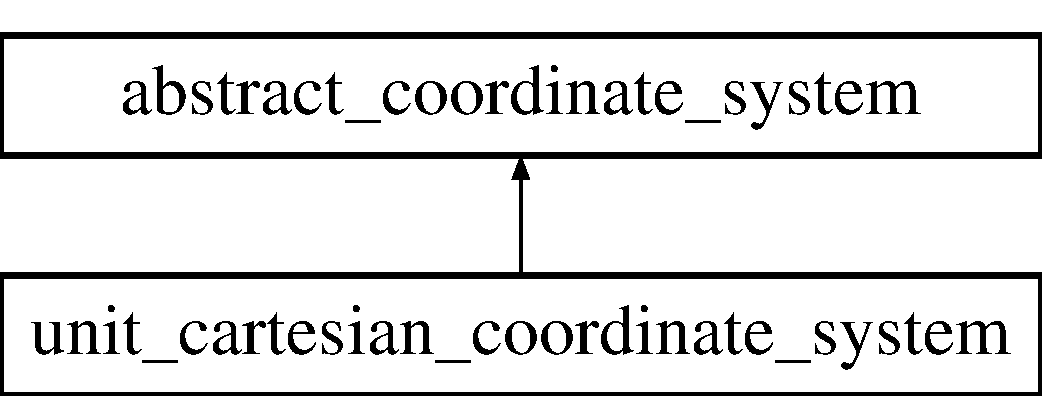
\includegraphics[height=2.000000cm]{classunit__cartesian__coordinate__system}
\end{center}
\end{figure}
\subsection*{Public Member Functions}
\begin{DoxyCompactItemize}
\item 
\hyperlink{classunit__cartesian__coordinate__system_a0a471305ff0743a900c9c270e52bd243}{unit\-\_\-cartesian\-\_\-coordinate\-\_\-system} ()
\item 
virtual void \hyperlink{classunit__cartesian__coordinate__system_a96d70a42cec4279c1320995e770c3fe5}{init} (sharedptr$<$ \hyperlink{classtile}{tile} $>$ t)
\item 
virtual float \hyperlink{classunit__cartesian__coordinate__system_a9093a6700e1a34f6dfb127358973c8c5}{calc\-\_\-delta\-\_\-x} (long iw, long ih)
\item 
\hypertarget{classunit__cartesian__coordinate__system_aa9cd14787ed2ca759ee7552dc799b9ba}{virtual float \hyperlink{classunit__cartesian__coordinate__system_aa9cd14787ed2ca759ee7552dc799b9ba}{calc\-\_\-delta\-\_\-y} (long iw, long ih)}\label{classunit__cartesian__coordinate__system_aa9cd14787ed2ca759ee7552dc799b9ba}

\begin{DoxyCompactList}\small\item\em See calc\-\_\-delta\-\_\-x\-\_\-at. \end{DoxyCompactList}\item 
\hypertarget{classunit__cartesian__coordinate__system_aeae04db199b3e27c57f955bccf8c3155}{virtual float \hyperlink{classunit__cartesian__coordinate__system_aeae04db199b3e27c57f955bccf8c3155}{get\-\_\-delta\-\_\-x} ()}\label{classunit__cartesian__coordinate__system_aeae04db199b3e27c57f955bccf8c3155}

\begin{DoxyCompactList}\small\item\em Special overloaded method that gives the equidistant space between points in x. \end{DoxyCompactList}\item 
\hypertarget{classunit__cartesian__coordinate__system_a8b6ec8c5b8230d1fcc79f9e9f1c365f1}{virtual float \hyperlink{classunit__cartesian__coordinate__system_a8b6ec8c5b8230d1fcc79f9e9f1c365f1}{get\-\_\-delta\-\_\-y} ()}\label{classunit__cartesian__coordinate__system_a8b6ec8c5b8230d1fcc79f9e9f1c365f1}

\begin{DoxyCompactList}\small\item\em See get\-\_\-delta\-\_\-x. \end{DoxyCompactList}\item 
\hypertarget{classunit__cartesian__coordinate__system_a765716f6eeb58e5340139f220f8e4649}{float \hyperlink{classunit__cartesian__coordinate__system_a765716f6eeb58e5340139f220f8e4649}{calc\-\_\-x\-\_\-at} (long iw, long ih)}\label{classunit__cartesian__coordinate__system_a765716f6eeb58e5340139f220f8e4649}

\begin{DoxyCompactList}\small\item\em Calculate x coordinate at given pixel. \end{DoxyCompactList}\item 
\hypertarget{classunit__cartesian__coordinate__system_ab45fbd73df0d1d3f4fe3bce0f65d2a8e}{float \hyperlink{classunit__cartesian__coordinate__system_ab45fbd73df0d1d3f4fe3bce0f65d2a8e}{calc\-\_\-y\-\_\-at} (long iw, long ih)}\label{classunit__cartesian__coordinate__system_ab45fbd73df0d1d3f4fe3bce0f65d2a8e}

\begin{DoxyCompactList}\small\item\em Calculate y coordinate at given pixel. \end{DoxyCompactList}\end{DoxyCompactItemize}


\subsection{Detailed Description}
This is a class that represents the unit cartesian coordinate system of a tile. For a given pixel coordinate iw,ih this class provides a method to obtain the x coordinate (corresponding to the width-\/direction) and the y coordinate of the pixel coordinate system. The coordinate system for this class is defined as such\-: Coordinates are given in (x,y)

(0,0)-\/-\/-\/-\/-\/-\/-\/-\/-\/-\/-\/-\/-\/-\/-\/---$>$(1,0) $\vert$ $\vert$ $\vert$ $\vert$ $\vert$ (x,y) (floating point values!) $\vert$ $\vert$ v v (1,0)-\/-\/-\/-\/-\/-\/-\/-\/-\/-\/-\/-\/-\/-\/-\/---$>$(1,1)
\begin{DoxyItemize}
\item These coordinates will hold even if the tile is N\-O\-T Q\-U\-A\-D\-R\-A\-T\-I\-C! This makes it easy to define model functions that live on this unit coordinate system indepedent of the shape and number of pixels of the tiles. 
\end{DoxyItemize}

\subsection{Constructor \& Destructor Documentation}
\hypertarget{classunit__cartesian__coordinate__system_a0a471305ff0743a900c9c270e52bd243}{\index{unit\-\_\-cartesian\-\_\-coordinate\-\_\-system@{unit\-\_\-cartesian\-\_\-coordinate\-\_\-system}!unit\-\_\-cartesian\-\_\-coordinate\-\_\-system@{unit\-\_\-cartesian\-\_\-coordinate\-\_\-system}}
\index{unit\-\_\-cartesian\-\_\-coordinate\-\_\-system@{unit\-\_\-cartesian\-\_\-coordinate\-\_\-system}!unit_cartesian_coordinate_system@{unit\-\_\-cartesian\-\_\-coordinate\-\_\-system}}
\subsubsection[{unit\-\_\-cartesian\-\_\-coordinate\-\_\-system}]{\setlength{\rightskip}{0pt plus 5cm}unit\-\_\-cartesian\-\_\-coordinate\-\_\-system\-::unit\-\_\-cartesian\-\_\-coordinate\-\_\-system (
\begin{DoxyParamCaption}
{}
\end{DoxyParamCaption}
)}}\label{classunit__cartesian__coordinate__system_a0a471305ff0743a900c9c270e52bd243}
Constructor. Before the coordinate system can be used, it has to be initialized with the given tile. Only after the init(...) method is called will the calculations functions give useful results. 

\subsection{Member Function Documentation}
\hypertarget{classunit__cartesian__coordinate__system_a9093a6700e1a34f6dfb127358973c8c5}{\index{unit\-\_\-cartesian\-\_\-coordinate\-\_\-system@{unit\-\_\-cartesian\-\_\-coordinate\-\_\-system}!calc\-\_\-delta\-\_\-x@{calc\-\_\-delta\-\_\-x}}
\index{calc\-\_\-delta\-\_\-x@{calc\-\_\-delta\-\_\-x}!unit_cartesian_coordinate_system@{unit\-\_\-cartesian\-\_\-coordinate\-\_\-system}}
\subsubsection[{calc\-\_\-delta\-\_\-x}]{\setlength{\rightskip}{0pt plus 5cm}float unit\-\_\-cartesian\-\_\-coordinate\-\_\-system\-::calc\-\_\-delta\-\_\-x (
\begin{DoxyParamCaption}
\item[{long}]{iw, }
\item[{long}]{ih}
\end{DoxyParamCaption}
)\hspace{0.3cm}{\ttfamily [virtual]}}}\label{classunit__cartesian__coordinate__system_a9093a6700e1a34f6dfb127358973c8c5}
This is a method that returns the distance between neighboring points at point iw,ih. It was implemented to enable calculating the gradient in non equidistant coordinate systems (Jacobian). Here it just returns a constant. 
\begin{DoxyParams}{Parameters}
{\em iw} & \\
\hline
{\em ih} & \\
\hline
\end{DoxyParams}
\begin{DoxyReturn}{Returns}
deltax 
\end{DoxyReturn}


Implements \hyperlink{classabstract__coordinate__system_a7df5507f5b2fddc0eb691e79514accab}{abstract\-\_\-coordinate\-\_\-system}.

\hypertarget{classunit__cartesian__coordinate__system_a96d70a42cec4279c1320995e770c3fe5}{\index{unit\-\_\-cartesian\-\_\-coordinate\-\_\-system@{unit\-\_\-cartesian\-\_\-coordinate\-\_\-system}!init@{init}}
\index{init@{init}!unit_cartesian_coordinate_system@{unit\-\_\-cartesian\-\_\-coordinate\-\_\-system}}
\subsubsection[{init}]{\setlength{\rightskip}{0pt plus 5cm}void unit\-\_\-cartesian\-\_\-coordinate\-\_\-system\-::init (
\begin{DoxyParamCaption}
\item[{sharedptr$<$ {\bf tile} $>$}]{t}
\end{DoxyParamCaption}
)\hspace{0.3cm}{\ttfamily [virtual]}}}\label{classunit__cartesian__coordinate__system_a96d70a42cec4279c1320995e770c3fe5}
This method initializes the coordinate system with the dimensions of the given tile. This method must be called before the calc\-\_\-... methods are called. 
\begin{DoxyParams}{Parameters}
{\em t} & \\
\hline
\end{DoxyParams}


Implements \hyperlink{classabstract__coordinate__system_a646c34b26579fa6f27ce00dcd8ab5951}{abstract\-\_\-coordinate\-\_\-system}.



The documentation for this class was generated from the following files\-:\begin{DoxyCompactItemize}
\item 
include/tiles/unit\-\_\-cartesian\-\_\-coordinate\-\_\-system.\-h\item 
src/tiles/unit\-\_\-cartesian\-\_\-coordinate\-\_\-system.\-cpp\end{DoxyCompactItemize}

%--- End generated contents ---

% Index
\newpage
\phantomsection
\addcontentsline{toc}{chapter}{Index}
\printindex

\end{document}
